%% abtex2-modelo-trabalho-academico.tex, v-1.9.2 laurocesar
%% Copyright 2012-2014 by abnTeX2 group at http://abntex2.googlecode.com/ 
%%
%% This work may be distributed and/or modified under the
%% conditions of the LaTeX Project Public License, either version 1.3
%% of this license or (at your option) any later version.
%% The latest version of this license is in
%%   http://www.latex-project.org/lppl.txt
%% and version 1.3 or later is part of all distributions of LaTeX
%% version 2005/12/01 or later.
%%
%% This work has the LPPL maintenance status `maintained'.
%% 
%% The Current Maintainer of this work is the abnTeX2 team, led
%% by Lauro César Araujo. Further information are available on 
%% http://abntex2.googlecode.com/
%%
%% This work consists of the files abntex2-modelo-trabalho-academico.tex,
%% abntex2-modelo-include-comandos and abntex2-modelo-references.bib
%%

% ------------------------------------------------------------------------
% ------------------------------------------------------------------------
% abnTeX2: Modelo de Trabalho Academico (tese de doutorado, dissertacao de
% mestrado e trabalhos monograficos em geral) em conformidade com 
% ABNT NBR 14724:2011: Informacao e documentacao - Trabalhos academicos -
% Apresentacao
% ------------------------------------------------------------------------
% ------------------------------------------------------------------------
\title{Classificação Sintática automatizada de textos em português brasileiro utilizando redes neurais recursivas}
% * <marlovss@gmail.com> 2018-01-29T20:05:55.647Z:
% 
% > Classificação
% Análise
% 
% ^.

\documentclass[
	% -- opções da classe memoir --
	12pt,				% tamanho da fonte
	openright,			% capítulos começam em pág ímpar (insere página vazia caso preciso)
	twoside,			% para impressão em verso e anverso. Oposto a oneside
	a4paper,			% tamanho do papel. 
	% -- opções da classe abntex2 --
	%chapter=TITLE,		% títulos de capítulos convertidos em letras maiúsculas
	%section=TITLE,		% títulos de seções convertidos em letras maiúsculas
	%subsection=TITLE,	% títulos de subseções convertidos em letras maiúsculas
	%subsubsection=TITLE,% títulos de subsubseções convertidos em letras maiúsculas
	% -- opções do pacote babel --
	english,			% idioma adicional para hifenização
	french,				% idioma adicional para hifenização
	spanish,			% idioma adicional para hifenização
	brazil				% o último idioma é o principal do documento
	]{abntex2}

% ---
% Pacotes básicos 
% ---
\usepackage{lmodern}			% Usa a fonte Latin Modern			
\usepackage[T1]{fontenc}		% Selecao de codigos de fonte.
\usepackage[utf8]{inputenc}		% Codificacao do documento (conversão automática dos acentos)
\usepackage{lastpage}			% Usado pela Ficha catalográfica
\usepackage{indentfirst}		% Indenta o primeiro parágrafo de cada seção.
\usepackage{color}				% Controle das cores
\usepackage{graphicx}			% Inclusão de gráficos
\usepackage{subfig}
\usepackage{microtype} 			% para melhorias de justificação
\usepackage{xcolor}
\usepackage[normalem]{ulem}
\usepackage{csquotes}           % para citações
\usepackage[printonlyused,withpage]{acronym} % para usar siglas
\usepackage{import}
\usepackage{longtable}
\usepackage[linguistics]{forest}
\usepackage{csvsimple}
% \usepackage{makebox}
% \usepackage{subfiles}           % para trabalhar com múltiplos arquivos
% \usepackage{graphicx}
% \graphicspath{{imagens/}{../imagens/}}
\usepackage{listings}
\usepackage{wrapfig}
\usepackage{caption}
% \usepackage{subcaption}
\usepackage{svg}
\usepackage{amsmath}
\usepackage{capt-of}




% ---
		
% ---
% Pacotes adicionais, usados apenas no âmbito do Modelo Canônico do abnteX2
% ---
\usepackage{lipsum}				% para geração de dummy text
\usepackage{mwe}

% ---

% ---
% Pacotes de citações
% ---
\usepackage[brazilian,hyperpageref]{backref}	 % Paginas com as citações na bibl
\usepackage[alf]{abntex2cite}	% Citações padrão ABNT
\usepackage{hyperref} % para referenciar hiperlinks (IMPORTANTE: tem que ser sempre o último)
% --- 
% CONFIGURAÇÕES DE PACOTES
% --- 

% ---
% Configurações do pacote backref
% Usado sem a opção hyperpageref de backref
\renewcommand{\backrefpagesname}{Citado na(s) página(s):~}
% Texto padrão antes do número das páginas
\renewcommand{\backref}{}
% Define os textos da citação
\renewcommand*{\backrefalt}[4]{
	\ifcase #1 %
		Nenhuma citação no texto.%
	\or
		Citado na página #2.%
	\else
		Citado #1 vezes nas páginas #2.%
	\fi}%
% ---


% ---
% Configurações de aparência do PDF final

% alterando o aspecto da cor azul
\definecolor{blue}{RGB}{41,5,195}

% informações do PDF
\makeatletter
\hypersetup{
 	%pagebackref=true,
	pdftitle={\@title}, 
	pdfauthor={\@author},
	pdfsubject={\imprimirpreambulo},
    pdfcreator={LaTeX with abnTeX2},
	pdfkeywords={abnt}{latex}{abntex}{abntex2}{trabalho acadêmico}, 
	colorlinks=true,       		% false: boxed links; true: colored links
	linkcolor=blue,          	% color of internal links
	citecolor=blue,        		% color of links to bibliography
	filecolor=magenta,      		% color of file links
	urlcolor=blue,
	bookmarksdepth=4
}
\makeatother
% --- 

% --- 
% Espaçamentos entre linhas e parágrafos 
% --- 

% O tamanho do parágrafo é dado por:
\setlength{\parindent}{1.3cm}

% Controle do espaçamento entre um parágrafo e outro:
\setlength{\parskip}{0.2cm}  % tente também \onelineskip


% ---
% compila o indice
% ---
\makeindex
% ---
% ---
% Capa

% ---
% Informações de dados para CAPA e FOLHA DE ROSTO
% ---
\titulo{Como Treinar seu Parser:\\ Classificação Sintática automatizada de textos em português}
\autor{Fernando Medeiros do Nascimento}
\local{Salvador\\Brasil}
\orientador{Prof. Dr. Marlo Vieira dos Santos e Souza}
\data{2019}
%\coorientador{Equipe \abnTeX}
\instituicao{%
  Universidade Federal da Bahia -- UFBA
  \par
  Instituto de Matemática e Estatística
  \par
  Departamento de Ciência da Computação}
\tipotrabalho{Trabalho de Conclusão de Curso}
% O preambulo deve conter o tipo do trabalho, o objetivo, 
% o nome da instituição e a área de concentração 
\preambulo{Projeto de trabalho de conclusão do curso de Bacharelado em Ciência da Computação, da Universidade Federal da Bahia.}
% --- 
% ---

% ---
% ----
% Início do documento
% ----
\begin{document}

\newcommand{\coment}[1]{\textcolor{red}{\textbf{Nota:~#1}}}
% Retira espaço extra obsoleto entre as frases.
\frenchspacing 
\imprimircapa

% ----------------------------------------------------------
% ELEMENTOS PRÉ-TEXTUAIS
% ----------------------------------------------------------
% \pretextual



% ---
% Folha de rosto
% (o * indica que haverá a ficha bibliográfica)
% ---
\imprimirfolhaderosto*
% ---

% % ---
% Inserir a ficha bibliografica
% ---

% Isto é um exemplo de Ficha Catalográfica, ou ``Dados internacionais de
% catalogação-na-publicação''. Você pode utilizar este modelo como referência. 
% Porém, provavelmente a biblioteca da sua universidade lhe fornecerá um PDF
% com a ficha catalográfica definitiva após a defesa do trabalho. Quando estiver
% com o documento, salve-o como PDF no diretório do seu projeto e substitua todo
% o conteúdo de implementação deste arquivo pelo comando abaixo:
%
% \begin{fichacatalografica}
%     \includepdf{fig_ficha_catalografica.pdf}
% \end{fichacatalografica}
% \begin{fichacatalografica}
% 	\vspace*{\fill}					% Posição vertical
% 	\hrule							% Linha horizontal
% 	\begin{center}					% Minipage Centralizado
% 	\begin{minipage}[c]{12.5cm}		% Largura
	
% 	\imprimirautor
	
% 	\hspace{0.5cm} \imprimirtitulo  / \imprimirautor. --
% 	\imprimirlocal, \imprimirdata-
	
% 	\hspace{0.5cm} \pageref{LastPage} p. : il. (algumas color.) ; 30 cm.\\
	
% 	\hspace{0.5cm} \imprimirorientadorRotulo~\imprimirorientador\\
	
% 	\hspace{0.5cm}
% 	\parbox[t]{\textwidth}{\imprimirtipotrabalho~--~\imprimirinstituicao,
% 	\imprimirdata.}\\
	
% 	\hspace{0.5cm}
% 		1. Parser.
%         2. Classificador.
% 		3. Português Brasileiro.
% 		I. Orientador.
% 		II. Universidade Federal da Bahia.
% 		III. Departamento de Ciência da Computação.
% 		IV. Classificação Sintática automatizada de textos em português brasileiro. \\
	
% 	\hspace{8.75cm} CDU 02:141:005.7\\
	
% 	\end{minipage}
% 	\end{center}
% 	\hrule
% \end{fichacatalografica}
% --- % Ficha bibliográfica
% \include{./1-elementos-pretextuais/folhaAprovacao}    % Folha de aprovação
% ---
% Dedicatória
% ---
\begin{dedicatoria}
    \vspace*{\fill}
    \centering
    \noindent
    \textit{Dedico esse trabalho a todos que já pensaram em desistir de tudo e recomeçar. Vocês provavelmente tinham razão de pensar assim. Se tiver oportunidade, jogue tudo pra cima.} \vspace*{\fill}
\end{dedicatoria}
% % ---       % Dedicatória
% ---
% Agradecimentos
% ---
\begin{agradecimentos}
    Este trabalho merecia a menção de um incontável número de pessoas. O que é impossível. Meus agradecimentos, então, vão para:
    
    Minha mãe. Obrigado por todo o amor. Eu vou fazer todo sacrificio valer a pena.
    
    Minha irmã e meu pai. Por todo o crescimento, obrigado.
    
    Minha companheira. Companheira de emoções, aventuras, e vida. Viver é mais fácil com você.
    
    Onix e Mago. Obrigado pela paciência.
    
    Meus amigos. Vocês não me ajudaram em nada (risos), mas este trabalho seria impossível sem vocês.
    
    Meu orientador. Obrigado por não desistir (até quando eu já tinha desistido).
    
    A UFBA. Resistir é preciso, se renovar também.

\end{agradecimentos}
% ---    % Agradecimentos
% ---
% Epígrafe
% ---
\begin{epigrafe}
    \vspace*{\fill}
	\begin{flushright}
		\textit{``Eu amo prazos. Adoro prazos. Adoro o barulho de vento que eles fazem quando os dias vão passando''\\
		Douglas Adams}
	\end{flushright}
\end{epigrafe}
% ---          % Epígrafe

% ---
% RESUMOS
% ---
    \pretextual
    % resumo em português
\setlength{\absparsep}{18pt} % ajusta o espaçamento dos parágrafos do resumo
\begin{resumo}

    Classificadores sintáticos automatizados (também conhecidos como \textit{parsers}) são um recurso computacional estudado 
    % há bastante tempo dentro da 
    na área de Processamento de Linguagem Natural. São dispositivos capazes de realizar a classificação morfossintática de sentenças escritas em linguagem natural. Apesar de serem estudados há bastante tempo, são poucos os \textit{parsers} disponíveis desenvolvidos para o processamento da língua portuguesa.
    
    % Existem \textit{parsers} baseados em regras, mas os mais conhecidos são os estatísticos, que precisam de um conjunto de dados adaptado, para que seja realizado o seu treinamento.
    Existem diversos métodos de \textit{parsing} baseados em regras pré-definidas na literatura. Porém, atualmente os métodos mais investigados se baseiam em métodos estatísticos.
    % , e baseados em dados. Os estatísticos, em particular, 
    Tais métodos necessitam de um conjunto de dados de entrada pé-classificados para serem treinados. Estes conjuntos de dados são chamados de bancos de árvores (\textit{treebanks}).
    
    Dada a existência prévia de \textit{treebanks} próprios para o processamento da língua portuguesa; e \textit{parsers} com boa performance, mas que não estão adaptados para esta mesma língua, 
    % Curiosamente, existe uma quantidade interessante de conjuntos de dados pré-classificados, em português, acessíveis ao público, que podem ser usados para treinar \textit{parsers}.
    propõe-se, então, o treinamento de um \textit{parser} conhecido, desenvolvido com foco na língua inglesa, com dados de treino da língua portuguesa. Para tal, será realizada a \textit{transdução} dos dados
    % da língua portuguesa para a língua inglesa, sem perda de informação lexical.
    nos seus respectivos formatos originais para o formato aceito pelo \textit{parser} escolhido, sem perda de informação lexical. 
    
    % Para tal, desenvolveu-se uma metodologia de adaptação entre \textit{treebanks}, de modo a gerar uma efetiva correlação entre conjuntos de dados distintos.

 \textbf{Palavras-chaves}: \textit{parsers}, classificador sintático, Língua Portuguesa, transdução.
\end{resumo}          % Resumo na língua vernácula
    % resumo em inglês
\setlength{\absparsep}{18pt} % ajusta o espaçamento dos parágrafos do resumo

\begin{resumo}[Abstract]
 \begin{otherlanguage*}{english}
    Parsers are a well-known computational resource in the Natural Language Processing area. However, it’s hard to find parsers for the Portuguese language.  While there are lots of rule-based parsing methods.
    
    Curiously, there is an interesting amount of pre-classified datasets for the Portuguese language, of easy access, that may be used for parsing training.
    % There are rule-based parsers, but the most know are the statistic ones, that need an adapted dataset for its training.
    
    In this work, we propose training a known parser, developed for the English language, with Portuguese language training data. For such, we \textit{transduce} the data of the original dataset format to the chosen parser dataset format, without lexical information loss.
    % portuguese language to english language, without lexical information loss.

   \vspace{\onelineskip}
 
   \noindent 
   \textbf{Key-words}: parsers, portuguese language, transduction.
 \end{otherlanguage*}
\end{resumo}          % Resumo em língua estrangeira
    
    % % ---
% % inserir lista de ilustrações
% % ---
\pdfbookmark[0]{\listfigurename}{lof}
\listoffigures*
\cleardoublepage
% % ---  
    
    
    % % ---
% % inserir lista de tabelas
% % ---
\pdfbookmark[0]{\listtablename}{lot}
\listoftables*
\cleardoublepage
% % ---          % Resumo em língua estrangeira

    % ---
% inserir lista de abreviaturas e siglas
% ---
\begin{siglas}  
    \item [CD] \textit{Corpus} de Destino. \textit{Corpora} cujas estruturas será reproduzido no processo de transdução
    \item[CETEM] \textit{Corpus de Extractos de Textos Electrónicos NILC}, Corpus criados pelo projeto Linguateca. Possui as variantes CETEMFolha e CETEMPublico.
    \item[CFG] \textit{Context Free Grammars}, Gramáticas Livres de Contexto
    \item[CLI] \textit{Command Line Interface}, \textit{softwares} que permitem a interação por meio do terminal de comandos do sistema.
    \item[CO] \textit{Corpus} de Origem. \textit{Corpora} que passarão pelo processo de transdução para se assemelharem a algum CD.
    \item[FAQ] \textit{Frequently Asked Questions}, perguntas mais frequentes
    \item[IA] Inteligência Artificial
    %   \item[OotB] \textit{Out-of-the-Box}, \textquote{fora da caixa}
    \item[PCFG] \textit{Probabilistic Context Free Grammars}, Gramáticas Livres de Contexto Probabilísticas
    \item[PLN] Processamento de Linguagem Natural
    \item[POS] \textit{Part of Speech}, Parte do Discurso
    \item[PTB] \textit{Penn TreeBank}
    %   \item[RNN] \textit{Recursive Neural Networks}, Redes Neurais Recursivas
    %   \item[RNR] Ver RNN
    \item[SP] \textit{Stanford Parser}
    \item[UD] \textit{Universal Dependencies}, projeto para criar \textit{tagsets} unificados para \textit{treebanks} de diversas línguas
  
\end{siglas}       % Lista de abreviaturas e siglas
    %% ---

% ---
% inserir lista de símbolos
% ---
% \begin{simbolos}
%   \item[$ \Gamma $] Letra grega Gama
%   \item[$ \Lambda $] Lambda
%   \item[$ \zeta $] Letra grega minúscula zeta
%   \item[$ \in $] Pertence
% \end{simbolos}
% ---     % Lista de símbolos

% ---
% inserir o sumario
% ---
\pdfbookmark[0]{\contentsname}{toc}
\tableofcontents*
\cleardoublepage
% ---

% ----------------------------------------------------------
% ELEMENTOS TEXTUAIS
% ----------------------------------------------------------
\textual
% ----------------------------------------------------------
% Introdução (exemplo de capítulo sem numeração, mas presente no Sumário)
% ----------------------------------------------------------
\chapter{Introdução}
\label{cap:introducao}
% ----------------------------------------------------------
% \begin{quote}
%     \textquote{O mundo é mediado pela linguagem} \cite{oliveira2019servico}
%     \footnote{É claro que uma reflexão tão bonita não teria sido gerada por mim. Muita gente já falou isso antes de mim, \citeonline{spolador2018mediadora} e \citeonline{baccega1995palavra} para citar exemplos.}
% \end{quote}
\textquote{O mundo é mediado pela linguagem} \cite{oliveira2019servico}
\footnote{Esta é um,  citar \citeonline{spolador2018mediadora} e \citeonline{baccega1995palavra} como referências.}
, no sentido que, interações humanas são realizadas a partir da linguagem, ou interpretadas com base nela. 
% \textquote{Mas e quando eu chuto uma pedra? Eu só uso a linguagem pra xingar ela!}.
Pode-se pensar, então, em situações nas quais a linguagem \textquote{não é} diretamente usada, como ao chutar uma pedra.
% Bom, você interpreta toda a situação se valendo da linguagem para fazê-lo. 
Porém, toda a situação é interpretada se valendo da linguagem para fazê-lo. 
A saber, quando se lembra do ocorrido, quando se comenta sobre etc. O falar, o ler e o ouvir tem peso fundamental no domínio da linguagem e, por conseguinte, na compreensão de mundo.

\citeonline[p~33]{fanon2008pele} afirma: \textquote{Falar é estar em condições de empregar uma certa sintaxe, possuir a morfologia de tal ou qual língua, mas é sobretudo assumir uma cultura, suportar o peso de uma civilização}. E complementa (\textit{\Ibidem[p~33]{fanon2008pele}}) \textquote{Um homem que possui a linguagem possui, em contrapartida, o mundo que essa linguagem expressa e que lhe é implícito}. Dominar a língua, ser capaz de interpretá-la e articulá-la, d
á ao indivíduo uma série de possibilidades. Não só o poder de influência, mas o poder do reconhecimento como pessoa, (\textit{\Ibidem[p~33]{fanon2008pele}}) \textquote{Uma vez que falar é existir absolutamente para o outro}.

% Não é de surpreender, portanto, que a partir do momento que possuímos ferramentas tão poderosas como computadores, desejemos que elas sejam capazes de falar e compreender linguagem humana. Este não é um desejo novo. Pelo contrário, 
Desde a origem da computação, existe o desejo em fazer com que computadores sejam capazes de processar linguagem.
Quando \citeonline[p~433]{turingJogoImitacao}, nos pede que consideremos a questão \textquote{Podem as máquinas pensar?},
% \textit{Can machines think?}}\footnote{\textquote{Podem as máquinas pensar?}. Tradução própria.}
a forma sugerida para que o famoso Jogo da Imitação seja operado é, essencialmente, uma troca de mensagens, ou seja, o uso livre da linguagem. 

% % Sendo um pouco mais pragmático, já 
% Em 1956 acontece o \textit{Dartmouth Summer Research Project on Artificial Intelligence}\footnote{\textquote{Projeto de Pesquisa de Verão em Inteligência Artificial de Dartmouth}. Tradução própria.}, em New Hampshire, Estados Unidos, que viria a ser conhecido como a origem da Inteligência Artificial (I.A.) como conhecemos hoje. Seu nome foi cunhado por um dos idealizadores, John Mccarthy. O evento termina sem uma concordância entre metodologias e problemas comuns da teoria geral. Pelo contrário, como vemos em \cite[p~87]{Moor2006DartmouthIA}, na proposta da conferência constava:
% \begin{quote}
%     \textquote{O estudo deve seguir com base da conjectura que todo aspecto do aprendizado ou qualquer outra característica da inteligência pode, em princípio, ser tão precisamente descrito, que uma máquina pode ser feita para simulá-lo.}
%     \footnote{ \textquote{\textit{The study is to proceed on the basis of the conjecture that every aspect of learning or any other feature of intelligence can in principle be so precisely described that a machine can be made to simulate it.}} Tradução própria.}
%     \footnote{Pode-se trazer visões distintas acerca do tópico. Turing, em \citeonline[p~442]{turingJogoImitacao} postula: \textquote{A visão popualr de que cientistas procedem inexoravelmente de fatos bem estabelecidos para fatos bem estabelecidos, nunca sendo influenciados por qualquer conjectura sem probas, é bastante errônea} (Tradução própria). 
%     % \textquote{The popular view that scientists proceed inexorably from well-established fact to well-established fact, never being influenced by any unproved conjecture, is quite mistaken}. 
%     Já Minsky como visto em \cite[p~87]{Moor2006DartmouthIA}, demonstra descontentamento com o andamento da área. \textquote{Minksy expressou a preocupação de que muitos na IA hoje em dia tentam fazer o que é popular e publicam apenas o que tem sucesso. Ele argumenta que IA nunca poderá ser uma ciência até que se publique o que falha assim como o que tem sucesso.} Tradução própria).
%     % \textquote{Minsky expressed the concern that too many in AI today try to do what is popular and publish only successes. He argued that AI can never be a science until it publishes what fails as well as what succeeds.}
%     }
% \end{quote}

A interpretação da linguagem por meios automáticos é uma das várias áreas que a Inteligência Artificial (I.A.) estuda, chamada de PLN (Processamento de Linguagem Natural, ou NLP em inglês). 
% Que pode atrair, obviamente, muitos olhares poderosos.
\citeonline{oquepln2017rodrigues} resume:
\begin{quote}
    \textquote{O objetivo do PLN é fornecer aos computadores a capacidade de entender e compor textos. \textquote{Entender} um texto significa reconhecer o contexto, fazer análise sintática, semântica, léxica e morfológica, criar resumos, extrair informação, interpretar os sentidos, analisar sentimentos e até aprender conceitos com os textos processados.}
\end{quote}

PLN é muito estudada como ciência de base, ou até mesmo por empresas para a criação de produtos como \textit{chatbots} e Assistentes Pessoais, para citar exemplos cotidianos. 
% Além disto, PLN pode ser estudado como recurso político e estratégico.

% Entre 1987 e 1997 aconteceram as \textit{Message Understanding Conference} (MUC)\footnote{\textquote{Conferência de Compreensão de Mensagens}. Tradução própria.}. Como visto em \cite[p~466]{Grishman1996MUC}, foram organizadas pela NRAD\footnote{\textquote{\textit{Naval Research And Development}}, Desenvolvimento e pesquisa Naval}, uma divisão da RDT\&E\footnote{\textquote{\textit{Research, Development, Test \& Evaluation}}, Pesquisa, Desenvolvimento, Teste e Avaliação} do Centro de Comando Naval, Controle, e Vigilância Oceânica (antiga NOSC, Centro de Sistemas Oceânico Navais), com apoio da DARPA, a Agência de Projetos de Pesquisa de Defesa Avançada. Na conferência, diversos testes eram feitos, onde os participantes recebiam provas de Extração de Informação, visando obter dados valiosos de documentos.\footnote{\textquote{Curiosamente}, já na sua terceira edição, o MUC-3, os documentos base se tornaram relatórios sobre terrorismo na América do Sul e Central, o que mostra a atenção política dada pelos EUA ao Cone Sul.}

% De quais formas podemos ensinar um computador a ler e escrever? Diversas, na verdade. 
Uma das formas de utilizar a linguagem computacionalmente é a Classificação Sintática Automatizada. Como definido por \citeonline[p~33]{charniak97statistical}, \textquote{Classificação sintática automatizada é o processo de atribuir um marcador de sintagma a uma sentença
\footnote{No original: \textit{Syntactic parsing is the process of assigning a phrase marker to a sentence}}
}.
% Ou seja, lembra na escola, quando você tinha que fazer a análise sintática de \textquote{João ganhou a bola}? 
Ou seja, realizar a análise sintática de sentenças como \textquote{João ganhou a bola} é definir, por exemplo, que João é substantivo, ganhou é verbo etc. Classificação automatizada diz respeito à construção de sistemas computacionais que realizem tal tarefa.

% Tenta-se, até hoje, achar
Ainda se pesquisam métodos baseados em lógica para realizar tal tarefa. Porém, 
% o que anda em voga 
a tendência atual são os métodos estatísticos. Como definido em \citeonline[p~37]{charniak97statistical},
\begin{quote}
    \textquote{Classificadores estatísticos funcionam atribuindo probabilidades para possíveis classificações (árvores) de uma sentença, localizando a árvore mais provável, e então apresentando tal árvore como resposta. Também, para construir um \textit{parser} estatístico, deve-se descobrir como (1) encontrar possíveis árvores, (2) atribuir probabilidades para elas, e (3) devolver a mais provável.}
    \footnote{No original: \textquote{\textit{Statistical parsers work by assigning probabilities to possible parses of a sentence, locating the most probable parse, and then presenting the parse as the answer. Thus, to construct a statistical parser, one must figure out how to (1) find possible parses, (2) assign probabilities to them, and (3) pull out the most probable one.}}}
    (Tradução própria)
\end{quote}
% E porque utilizar a estatística, ao invés de regras bem estabelecidas? 
Para que tenham bom funcionamento, \textit{parsers} precisam ser treinados com um conjunto de sentenças pré-classificadas. A essas sentenças damos o nome de \textit{árvores}, e ao seu conjunto, o nome de Banco de Árvores, ou \textit{treebanks} (como serámelhor explicado em \ref{sec:parser}).

Ao leitor pode parecer contra-intuitivo, utilizar estatística ao invés de regras pré-definidas. Nas palavras do próprio Charniak, em \cite[p~89]{Moor2006DartmouthIA}:
\begin{quote}
    \textquote{Estatística dominou o processamento de linguagem natural porque funciona}
    \footnote{\textquote{\textit{Statistics has taken over natural language processing because it works.}}}
    (Tradução própria)
\end{quote}
% Como vemos em \cite{kegler2019parsing}, é possível retomar o histórico do estudo de \textit{parsers}\footnote{\textit{\textit{parser}} é o equivalente a classificador sintático na língua inglesa.} a períodos anteriores à era comum,
% mas vamos nos reduzir aos estudos de Ada Lovelace em 1854, com a primeira linguagem de programação, e aos estudos do sr. Rutishauser em 1949, com o primeiro compilador teórico. 
% mas podemos tomar como partida os estudos do Sr. Rutishauser. 
% Pode-se dizer, então, que os estudos sobre \textit{parsers} ocorrem desde 1949, pelo menos.
Por \cite{kegler2019parsing}, conseguimos traçar os estudos modernos de \textit{parsing} desde 1949. 
% \textit{Parsers} tem largo uso tanto para a área de Compiladores, como de PLN (falamos disso em \ref{sec:parsing}). 
Uma busca simples no Google Acadêmico\footnote{scholar.google.com.br} por \textquote{\textit{parser}} nos retorna aproximadamente 320.000 resultados. Pesquisar por \textquote{\textit{natural language processing}} retornará aproximadamente 3.290.000. \textit{Parsers} são quase 10\%
% \footnote{Na verdade, são 9.72\%. Mas você não faz muitos amigos levando as coisas tão ao pé da letra.} 
deste total.

% Uma área tão antiga, certamente tem estudos para o português.
% \footnote{Por que o foco no português? Porque os autores são brasileiros.} 
Fazendo um processo semelhante, buscando por \textquote{\textit{\textit{parser} portuguese}}\footnote{classificador sintático português}, obtemos aproximadamente 10.400 resultados. Quase 3\%.
% Para tantos idiomas no mundo, não é ruim.
% Existem diversos idiomas no mundo, é uma boa fatia.
Já \textquote{classificador sintático português} retorna 15.100 resultados. A pesquisa por  \textquote{\textit{parser english}}, porém, retorna 106.000 resultados. O triplo de resultados em comparação com o verbete anterior.

% Note, não é o objetivo deste trabalho um embate entre lusófonos e anglófonos. Mas, de fato, as pesquisas em PLN sobre a língua portuguesa ainda estão longe de alcançarem números tão expressivos. Claro, a pesquisa existe, é crescente, e demonstra grande entusiasmo e comprometimento dos pesquisadores. No STIL\footnote{\textquote{Symposium in Information and Human Language Technology}, Simpósio em Informação e Tecnologia de Linguagem Humana --  \url{http://www.bracis2019.ufba.br/index.html}} 2019, por exemplo, uma quantidade considerável de trabalhos visava a interpretação, ou o auxílio à pesquisa da língua portuguesa (na forma da criação de \textit{datasets}, por exemplo), com alto nível de qualidade. Existe interesse nos estudos para esta linguagem. Mas, usando o mesmo evento como um micro estudo de caso, poucos trabalhos envolviam a pesquisa com \textit{parsers}\footnote{\url{http://comissoes.sbc.org.br/ce-pln/stil2019/accepted.html}}. O que gerou esse desinteresse? Hipótese:
% \begin{quote}
%     Desenvolver \textit{parsers} não é trivial, mesmo com dados e métodos disponíveis.
% \end{quote}

É compreensível que o número de pesquisas na área para a língua inglesa seja maior do que em português. É importante que se diga, também, que existem \textit{treebanks} robustos para o português. Sente-se falta da conexão entre ambos, \textit{parsers} e dados. Pode-se criar a hipótese, portanto, de que mesmo com dados e métodos disponíveis, o desenvolvimento de \textit{parsers} não é trivial. Isso explicaria a tendência (natural) dos pesquisadores de dedicarem maior esforço para os métodos já desenvolvidos, além de focar em língua com maior expressão global.

Dada a complexidade da tarefa, surge a inquietação que motiva este trabalho: Seria possível desenvolver um \textit{parser} \textit{out-of-the-box}, ou seja, tentando utilizar apenas materiais já desenvolvidos (a saber, \textit{parsers} já existentes, bem como corpus de treino já existentes), de modo que ele seja eficiente?

Sobre \textit{out-of-the-box parser}, seguimos a linha de \citeonline[p~2]{Branco2010OutOfTheBox}, que se propõe a estender pacotes de \textit{software} já disponíveis, que permitam treinar um \textit{parser} robusto a partir de um \textit{treebank}, que seja independente de linguagem e suporte uma aplicação para o português sem grandes problemas.

% Já abordamos as três partes da sentença nessa introdução.
% Como já vimos: O desenvolvimento de \textit{parsers} é bastante expressivo, mas exige tempo e recursos; existem dados que podem ser usados na língua portuguesa, e vêm sendo desenvolvidos cada vez mais; e a comunidade científica já lida com o desenvolvimento deles há bastante tempo. Tem um detalhe, ainda não declarado: é um conhecimento ainda \textquote{fechado} à comunidade científica, e à grandes empresas de tecnologia. 
% % O público geral não conseguiria começar a estudar o desenvolvimento de \textit{parsers} com a mesma praticidade e acolhimento que pessoas que começam a desenvolver \textit{websites}, por exemplo. 
% O público geral conseguiria começar a estudar o desenvolvimento de \textit{parsers} sem grandes dificuldades? De modo semelhante às pessoas que começaram a desenvolver \textit{websites}, por exemplo?
% Temos algumas questões em mãos, e várias delas apresentam dificuldades que podem ser exploradas.
% % vamos explorar essas dificuldades!

% Como já foi dito, vários métodos e vários materiais já existem, e estão disponíveis publicamente para acesso e uso. Porque não trabalhar com isto? Poderíamos usar algum \textit{parser} 
% % em inglês,
% já conhecido, que é utilizado para outras línguas, como a língua inglesa,
% dados em português, e pronto, o sucesso nos aguarda.

% Infelizmente, como espera-se que fique claro com este trabalho, não é simples fazer tal tarefa. Para serem utilizados, \textit{parsers} recebem implementações específicas para a língua que foram desenvolvidos. Mais do que isso, esperam informações que já estejam em formatos específicos, e estes, muitas vezes, são pensados para sua língua de origem, não para idiomas de forma geral.
% Mas essa ideia ainda é boa demais para ser desperdiçada.
% Podemos, então, tentar outra abordagem.
% Porque não \textit{transduzimos} os dados?
Os primeiros testes empíricos foram um fracasso. Os corpus disponíveis não eram recebidos pelos \textit{parsers} que localizamos. Levantou-se, então, uma nova possibilidade: realizar a transdução dos dados de entrada.  
    
% \textquote{Ei, você escreveu errado, é \textquote{traduzir}!}

\textquote{Transdutores} foram explicados por \citeonline[p~1]{weightedTransducersMohri}:
\begin{quote}
    \textquote{[Transdutores] São autômatos os quais cada transição, em adição à sua etiqueta de entrada normal, é aumentado com uma etiqueta de saída de um possível novo alfabeto, e carrega algum elemento de peso de um semi anel. Transdutores podem ser usados para definir um mapeamento entre dois tipos diferentes de fontes de informação, por exemplo palavras e sequências de fenômenos}
    \footnote{\textquote{\textit{[Transductors] are automata in which each transition in addition to its usual input label is augmented with an output label from a possibly new alphabet, and carries some weight element of a semiring. Transducers can be used to define a mapping between two different types of information sources, e.g., word and phoneme sequences.}}}
    (Tradução própria)
\end{quote}

% Ou seja, vamos transduzir um conjunto de dados n’outro. Porque não só \textquote{traduzir}? 
% % Porque linguas diferentes têm características diferentes, e precisamos estar prontos para lidar com elas.
% Porque línguas distintas possuem especificidades que tornam complexo o processo de tradução direta. Não só isto, mas como veremos nas próximas páginas, os próprios conjuntos de dados possuem características muito peculiares.
Em suma, neste trabalho, faremos a transdução de conjuntos de dados construídos num certo formato, para um novo formato, e faremos a avaliação deste experimento. Isto nos leva a um segundo produto: o desenvolvimento de uma metodologia de adaptação inter-corpora.

% Após esta introdução, vamos definir o que é cada conceito do projeto, e suas etapas de execução, além de seus resultados.

    
\section{Contexto do Trabalho}
\label{sec:contexto}

O estudo de \textit{parsers} é bastante conhecido do meio acadêmico, tendo muito uso tanto na NLP, como na compilação de linguagens de programação. Também, existe uma produção crescente para o desenvolvimento de tecnologias em NLP para o português, principalmente para as variantes europeia e brasileira. 
% Porém, o estudo de \textit{parsers} para a língua portuguesa parece não receber o mesmo entusiasmo, ficando restrito à melhoria dos sistemas já conhecidos.
Foi sentida, porém, a falta de mais estudos focados na língua portuguesa.

Pesquisas prévias mostraram que existem, sim, \textit{parsers} projetados pensando na língua portuguesa (serão mais abordados na sessão \ref{subsec:parser_portugues}). Porém, eram de difícil acesso, ou não era possível utilizá-los. Foram encontrados, também, bancos de dados\footnote{Bancos de Árvores (\textit{treebanks}, que serão melhor explicados em (\ref{sec:treebank})} com dados da língua portuguesa, variantes europeia e brasileira.

Sabendo-se da existência de tecnologias tanto de \textit{parsing} como de textos em português pré-classificados, pensou-se na possibilidade do desenvolvimento \textit{Out-of-the-box}, adaptando tecnologias pré-existentes, e avaliando seus resultados. Não apenas desejando verificar a eficiência de tal método, como analisar quanto estudo técnico é necessário para tal.

Notou-se, contudo, que tal processo de adaptação exige um método ele mesmo. Pois os \textit{parsers} exigem um formato de entrada, que nem sempre é o mesmo formato dos dados disponíveis.

Portanto, foi desenvolvido um método que faça a conversão entre dados de formatos distintos, de modo a que seja possível o uso destes dados no analisador sintático escolhido.

% Com isto queremos, com pouco desenvolvimento, adaptar um \textit{parser} já estabelecido para a língua portuguesa. 

% Por que pouco desenvolvimento? Porque queremos, também, verificar o quão simples seria, para alguém sem conhecimento acadêmico, realizar tal feito.


\section{Objetivo Geral}
\label{sec:objetivos-gerais}
%o que vc quer fazer 
% v1
% O objetivo deste trabalho é transduzir conjuntos de dados do português para o inglês, e verificar se um \textit{parser} conhecido e já utilizado é capaz de ter boa performance, quando recebendo dados de outro idioma para o qual não foi desenvolvido primariamente.
% O objetivo deste trabalho é realizar o treinamento de um \textit{parser} estabelecido, a partir de técnicas \textit{out-of-the-box}\footnote{\textquote{Fora da Caixa}, tradução própria.}, utilizando o mínimo de implementação. Verificar a capacidade de execução deste \textit{parser} a partir de conjuntos de treino originalmente não projetados para este classificador.

% v2
% Este trabalho possui dois objetivos principais. Primeiramente, deseja-se utilizar um \textit{parser} já existente e treiná-lo para a língua portuguesa, utilizando corpora também já existentes da língua portuguesa, e adaptando-os. Em segundo lugar, visa-se a criação de uma metodologia que auxilie o processo de transdução inter-corpora.

Este trabalho tem como objetivo o treinamento de \textit{parsers} já existentes para que sejam capazes de processar a língua portuguesa. A partir de tal treino, avaliar a sua eficiência, taxa de erros e afins.

\section{Objetivos Específicos}
\label{sec:objetivos-especificos}
\begin{itemize}
%quebrar o problema grande em subproblemas
    \item Estudar sobre analisadores sintáticos (\textit{parsers});
    \item Fazer o levantamento de florestas sintáticas (\textit{treebanks}) disponíveis na língua portuguesa;
    \item Fazer o levantamento de \textit{parsers} em português;
    \item Definir um \textit{parser} convencional a ser utilizado na pesquisa;
    \item Desenvolver um método de adaptação entre florestas sintáticas; 
    \item Realizar a adptação de florestas sintáticas para utilizar no \textit{parser} definido;
    \item Treinar o \textit{parser} definido com as florestas sintáticas adaptadas;
    \item Avaliar resultados do \textit{parser};
    % \item Testar \textit{parser} com sentenças específicas.
    
\end{itemize}

\section{Justificativa}	
\label{justificativa}

% Ao debater o Processamento de Linguagem Natural, \citeonline[p~10]{vieira2001linguistica} comentam:
% \begin{quote}
%     \textquote{Para lidar com os vários problemas, temos hoje, em nível mundial, uma comunidade científica e acadêmica em crescimento. Há muita pesquisa e trabalhos realizados principalmente para o Inglês, Espanhol, Alemão, Francês e Japonês. Encontramos, porém, carência de pesquisas, ferramentas, recursos linguísticos e humanos para tratar computacionalmente a língua portuguesa.}
% \end{quote}

Como já citado, a quantidade de pesquisas em \textit{parsers} para a língua portuguesa ainda estão em número reduzido com relação aos estudos mundiais. Por observação empírica, nota-se que estão muito focados na reprodução e manutenção de materiais já existentes, e antigos.
\cite[p~371]{Manning1999FoundationsNLP}:
\begin{quote}
    \textquote{Uma avaliação completa de classificadores como pré-processadores úteis para tarefas de NLP multilíngues de alto nível só serão possíveis após resultados experimentais suficientes de uma ampla gama de línguas estiver disponível}
    \footnote{No original: \textquote{\textit{A full evaluation of taggers as useful preprocessors for high-level multilingual NLP tasks will only be possible after sufficient experimental results from a wide range of languages are available.}}}
    (Tradução própria.)
\end{quote}

% Deseja-se que este seja mais um trabalho a acrescentar e fomentar conteúdo para esta subárea de pesquisa.


\section{Metodologia}
\label{sec:metodologia}
% O método utilizado para elaboração deste trabalho de conclusão de curso, foi: estudar conjuntos de sentenças já classificadas na língua portuguesa (\textit{treebanks}, serão explicados em \ref{treebank}), e verificar as correspondências destas com o formato aceito pelo \textit{parser} escolhido. A partir de então, verificar quais etiquetas morfossintáticas (\textit{POS tags}, abordadas em \ref{subsec:POStags}) tem correspondência direta, e quais não. As que possuem, foram feitas transduções diretas. As que não, verificar uma correspondência gramatical, e utilizá-las no procedimento. 

% Certas estruturas gramaticais são distintas, por mais que possuam valor sintático semelhante. Para estas, foi necessário fazer a convergência de estrutura, transduzindo assim não só as etiquetas, mas também a morfologia da árvore classificada (\textit{parse tree}, explicadas em \ref{parsing}).

% As sentenças classificadas e transduzidas foram utilizadas para treinar o \textit{parser}. Foram coletados os dados de resultados dos treinos e testes, e e feitas análises baseadas nos métodos abordados em \ref{resultados}. 

O desenvolvimento deste trabalho foi dividido em 6 etapas.

A Primeira etapa consistiu na revisão bibliográfica. Fez-se necessário o estudo dos classificadores sintáticos, e das florestas sintáticas. 

Para o estudo dos classificadores sintáticos, pesquisou-se no Google Acadêmico\footnote{\url{http://www.scholar.google.com}} por \textit{parsing}, \textit{statistical parsing}, \textit{constituency parsing}, \textit{Neural Networks and parsing}, \textit{Treebank}, \textit{parser comparison}. Foram coletados 10 artigos por assunto pesquisado, que tiveram seu resumo/\textit{abstract} lidos, para avaliação de relevância. Como material base de estudo, foi usado  \cite{Manning1999FoundationsNLP}. Será melhor abordado em \ref{sec:parser}.

Para a pesquisa de florestas sintáticas para o português, pesquisou-se pelas palavras-chave \textit{portuguese treebank}, \textit{treebank português}, \textit{floresta sintática português} em motores de busca como Google Acadêmico e Google\footnote{\url{www.google.com}}. Encontramos o Bosque \cite{bick2008FlorestaSintatica}, do projeto Floresta Sintá(c)tica disponível publicamente, e nos foi cedido o CINTIL \cite{cintil_handbook}. Será explicado em \ref{sec:treebank}.

De forma análoga, pesquisou-se por \textit{parsers} na língua portuguesa nos motores de busca supracitados, com as palavras-chave \textit{portuguese parser}, \textit{parser português}, \textit{classificador sintático português}. Encontramos referências ao PALAVRAS \cite{bick2000palavras} e ao LX-Parser \cite{siteLxParser}. Abordados em \ref{subsec:parser_portugues}.

Na Segunda etapa, buscou-se por um \textit{parser} a ser utilizado no projeto. Utilizando-se os motores de busca supracitados, pesquisou-se por \textit{parser}, \textit{parsing}, \textit{constituency parser}. Devido à sua robustez, fácil utilização sem necessidade de desenvolvimento (por comandos de terminal), e por ter amplo reconhecimento na comunidade, optou-se pelo uso do Stanford Parser \cite{fastAccurate}. Este recebe, como entrada, dados no formato Penn Treebank \cite{buildingPTB}. O SP será melhor descrito em \ref{sec:stanfordParser}.

% Para os \textit{parsers} convencionais, utilizamos os motores de busca supracitados, pesquisando por \textit{parser}, \textit{parsing}, \textit{constituency parser}. Durante a revisão de literatura, e em diálogos com especialistas, conhecemos o \textit{Stanford Parser}, que utiliza dados no formato \textit{Penn treebank}. Optamos por utilizá-lo.

Percebeu-se, então, a necessidade de realizar uma adaptação entre bancos de árvores, iniciando-se a Terceira etapa, de referencial teórico para a transdução.

Para a adaptação entre bancos de árvores, estudou-se a estrutura dos bancos originais, por observação de exemplos. De acordo com as necessidades observadas, estudamos os manuais de cada um, que conste: O Manual de \textit{bracketing} do Penn Treebann \cite{bracketing_ptb}, Manual de classificação do Penn Treebank \cite{buildingPTB}, Manual da Bíblia Florestal \cite{freitas2007biblia} e Manual de LxParser \cite{siteLxParser}. Com a necessidade de aprofundamento, estudou-se também o manual do formato 
Árvores Deitadas, utilizado no BOSQUE \cite{afonso2006arvores} e o Manual do Cintil \cite{cintil_handbook}. Neste contexto, foi desenvolvida a metodologia de transdução de \textit{parsers}, que será abordada neste trabalho. 

Na Quarta etapa, foi feita a transdução de bancos de árvores propriamente dita. O \textit{transdutor} foi desenvolvido na linguagem Python, pela afinidade do autor com a mesma. O desenvolvimento teve como objetivo realizar a transdução de modo a conservar a informação lexical dos dados originais, adaptando apenas a sua estrutura para que possam ser consumidos pelo supra-citado Stanford Parser. Como dito anteriormente, este \textit{parser} recebe como entrada árvores no formato Penn Treebank (PTB). Portanto, os bancos de árvores selecionados na etapa Um foram transduzidos para o formato PTB.
% Em casos onde foi obrigatória a adaptação do formato da sentença classificada, esforçou-se para realizar o mínimo de impacto na árvore resultante. 
A discussão aprofundada do método de transdução será realizada no Capítulo \ref{cap:desenv}.

A Quinta etapa envolveu o treino do Stanford Parser propriamente dito. Em nenhum momento houve implementação sobre o \textit{parser}. Foi realizado apenas o processo de transdução, treinamento e avaliação. Para o uso do \textit{parser}, foi utilizada a sua interface de terminal (\textit{command line interface}, CLI). O treino foi feito utilizando o método \textit{10-fold validation}, para possibilitar uma média de avaliação. Os procedimentos de treino serão comentados nas sessões \ref{sec:treinando_sp_cintil} e \ref{sec:treinando_sp_bosque}.

% As sentenças pré-classificadas transduzidas foram utilizadas para treinar o \textit{parser} escolhido. Optou-se por não realizar desenvolvimento de código diretamente sobre \textit{parser}. Portanto, foi utilizada a interface por terminal (\textit{command line interface}, CLI). Usou-se o método \textit{10-fold validation}, para obter diversas métricas de treino, que pudessem ser comparadas entre si, e com os resultados do outro conjunto de dados transduzidos.

% O classificador em questão imprime os resultados de treino por padrão. Tais resultados foram coletados, catalogados, e analisados. A análise foi feita, primeiramente, separando os resultados de cada conjunto de dados, e depois comparando-os.
Por fim, na Sexta etapa foi feito o cruzamento dos dados obtidos, suas análises e considerações, que serão demonstradas na sessão \ref{sec:resultados}.  % introdução



% % ---
% % Capitulo com exemplos de comandos inseridos de arquivo externo 
% % ---
% \include{abntex2-modelo-include-comandos}
% % ---


% ----------------------------------------------------------
% PARTE
% ----------------------------------------------------------
\part{Referenciais teóricos}
% ----------------------------------------------------------
% ---
% Capitulo de revisão de literatura
% ---

\chapter{Revisão de Literatura}

Para o bom entendimento do trabalho, é necessário que se explique os nomes, conceitos, e ferramentas utilizadas para o desenvolvimento deste trabalho.

Primeiramente, apresentamos conceitos linguísticos na sessão \ref{sec:parsing}. Em seguida, na sessão \ref{treebank}, estudamos os \textit{treebanks}: o que são, suas estruturas, e os \textit{treebanks} utilizados neste trabalho, tanto os que serão transduzidos, como o \textit{treebank} de referência. Por fim, em \ref{sec:parser}, explicamos os  \textit{parsers}: seu funcionamento, o \textit{parser} que utilizaremos para o estudo, alguns \textit{parsers} da língua portuguesa, e mostramos algumas formas de avaliação.

\section{Análise Sintática (\textit{Parsing})}
\label{sec:parsing}

Análise sintática, ou \textit{parsing}, é uma técnica que possui importância principalmente em duas áreas de conhecimento. A primeira, no campo do processamento de Linguagens de Computação. Na segunda, no campo do Processamento de Linguagens Naturais.

Sobre linguagens de computação, \citeonline[p~39]{aho2008compiladores} definem a análise sintática como \textquote{O processo para determinar como uma cadeia de terminais pode ser gerada por uma gramática}. Terminais são, na sua definição, (\textit{\Ibidem[p~27]{aho2008compiladores}}) \textquote{os símbolos elementares da linguagem, definidos pela gramática}. Sobre gramática, (\textit{\Ibidem[p~39]{aho2008compiladores}}) \textquote{descreve [\ldots] a estrutura hierárquica da maioria das construções de linguagens [\ldots]}. 

Já sobre Processamento de Linguagem Natural (que será dado foco neste trabalho), como descrito por \citeonline[p~33]{charniak97statistical}, \textit{parsing} é \textquote{\textit{the process of assigning a phrase marker to a sentence}} \footnote{\textquote{O processo de atribuir marcadores de frase a uma sentença}. Tradução própria}. Por exemplo, na frase \textquote{\textit{o cachorro late}}, \textit{o} pode ser marcado como artigo, \textit{cachorro} como substantivo, \textit{late} como verbo. \textit{O cachorro}, juntos, formam um sintagma nominal. O verbo, sozinho, faz parte de um sintagma verbal. E ambos formam a sentença. Como fica mais claro na Figura \ref{fig:parse-simple}.

\begin{center}
    \begin{figure}[h!]
    \centering
    % \includegraphics{}
    \begin{forest}
        [S
            [NP
                [artigo
                    [\textit{o}]
                ]
                [substantivo
                    [\textit{cachorro}]
                ]
            ]
            [VP
                [verbo
                    [\textit{late}]
                ]
            ]
        ]
    \end{forest}
    \caption[Exemplo de árvore simples]{Exemplo de árvore simples (Adaptado de \citeonline[p~34]{charniak97statistical})}
    \label{fig:parse-simple}
\end{figure}
\end{center}

A esta estrutura damos o nome de \textit{árvore de derivação}, \textit{árvore}, ou \textit{parse}.

Para sentenças simples, este é um trabalho simples. Porém, muito facilmente uma frase pode gerar mais de uma árvore, ou seja, gerar uma ambiguidade sintática\footnote{Nota: Não haverá foco na ambiguidade lexical neste trabalho.}, como no exemplo usado por \citeonline[p~10]{paganiavaliaccao}, na Figura \ref{fig:parse-ambiguity}

\begin{center}
    \begin{figure}[h!]
    \centering
    % \includegraphics{}
    Para a sentença \textquote{\textit{Arlindo tirou os pés da mesa}}:
    
    \textbf{a)}
    \begin{forest}
        [S
            [SN
                [\textit{Arlindo}]
            ]
            [SV
                [V
                    [\textit{tirou}]
                ]
                [SN
                    [SN
                        [\textit{os pés}]
                    ]
                    [SP
                        [\textit{da mesa}]
                    ]
                ]
            ]
        ]
    \end{forest}
    
    \textbf{b)}
    \begin{forest}
        [S
            [SN
                [\textit{Arlindo}]
            ]
            [SV
                [V
                    [\textit{tirou}]
                ]
                [SN
                    [\textit{os pés}]
                ]
                [SP
                    [\textit{da mesa}]
                ]
            ]
        ]
    \end{forest}
    \textbf{c)}
    \begin{forest}
        [S
            [SN
                [\textit{Arlindo}]
            ]
            [SV
                [SV
                    [V
                        [\textit{tirou}]
                    ]
                    [SN
                        [\textit{os pés}]
                    ]
                ]
                [SP
                    [\textit{da mesa}]
                ]
            ]
        ]
    \end{forest}
    
    \caption[Exemplo de ambiguidade entre árvores]{Exemplo de ambiguidade entre árvores (Adaptado de \citeonline[p~10]{paganiavaliaccao})}
    \label{fig:parse-ambiguity}
\end{figure}
\end{center}

Além da ambiguidade, existe outro problema: a quantidade de árvores incoerentes. Como destaca \citeonline[p~33]{charniak97statistical}, o exemplo 
\textquote{\textit{[\ldots] Implica que podemos atribuir pelo menos um significado semi-plausível para toda árvore possível. Para a maioria das gramáticas [\ldots], este não é o caso}
\footnote{No original: \textquote{[\ldots] implies that we can assign at least a semiplausible meaning to all the possible parses. For most grammars [\ldots], this is not the case.} Tradução própria.}}.
Ou seja, é necessário filtrar as árvores com real relevância e que mais se aproximem de uma estrutura correta.

Nesse ponto, existem métodos que resolvam essa ambiguidade, como as Gramáticas Lives de Contexto Probabilísticas e a classificação lexicalizada. Ambos serão abordados, respctivamente, nas sessões \ref{subsec:statisticalparsing} e \ref{subsec:lexParsing}.

O leitor pode se questionar qual a utilidade de \textit{parsing}, e do seu estudo. \citeonline{Manning1999FoundationsNLP} dedicam alguns capítulos para demonstrar seu uso e técnicas\ como Tradução de Máquina, Agrupamento (\textit{clustering}), Recuperação de Informação e Categorização de Textos. Entrar nestes assuntos escaparia ao escopo deste trabalho, mas recomendamos a leitura\footnote{\cite[capítulos~13,14,15,16]{Manning1999FoundationsNLP}}.

% Apesar de uma ferramenta muito útil e desafiadora, \citeonline[p~457]{Manning1999FoundationsNLP} destacam:
% \textquote{\textit{Partly because parsers do not perform well enough yet, parsing has rarely been applied to higher-level tasks like speech recognition and language understanding}}
% \footnote{\textquote{Em partes por ainda não performarem bem o bastante ainda, \textit{parsing} raramente vem sendo aplicado para tarefas de alto nível como reconhecimento de fala e compreensão de linguagem}. Tradução própria.}. 

% ---------------------------------------------------------

\subsection{Etiquetas Morfosintáticas - Part of Speech Tags}
\label{subsec:POStags}

Sintaticamente falando, palavras podem ser agrupadas em classes (ou grupos) que demonstrem seu comportamento sintático. Tais classes podem ser chamadas de Categorias Sintáticas, ou Categorias Gramaticais. Mesmo Classes. Exemplos de classes são \textit{verbo}, \textit{substantivo}, \textit{adjetivo}, \textit{artigo} etc. Outra forma de se referir a tais classes, é chamando-as de \textquote{\textit{Part of Speech}}\footnote{Parte do Discurso} (POS).

% Como saber se palavras diferentes pertencem ao mesmo grupo? 
\cite[p~81]{Manning1999FoundationsNLP} \textquote{O teste mais básico para palavras pertencentes à mesma classe é o teste de substituição}
\footnote{No original: \textquote{\textit{The most basic test for words belonging to the same class is the substitution test.}} Tradução própria.}.
Podemos ver um exemplo na Figura \ref{fig:substTest}.

\begin{center}
\begin{figure}[h!]
    \centering
    % \includegraphics{}
    \begin{tabular}{c c c}
        A &
        %  \[ 
        \begin{math}
            \left \{
                \begin{tabular}{c}
                    casa\\
                    pessoa\\
                    mulher\\
                    criança\\
                    Bolsa de Valores\\
                    pena\\
                \end{tabular}
            \right \}
            % \] 
        \end{math}
            & caiu.\\
    \end{tabular}
    
    \caption[Teste de Substituição]{Teste de Substituição}
    \label{fig:substTest}
\end{figure}
\end{center}

Na Figura \ref{fig:substTest}, demonstramos o teste da substituição para substantivos. Note que palavras podem ter mais de uma POS. Por exemplo, \textit{casa} pode ser um substantivo (NN), ou a terceira pessoa do singular do verbo \textquote{casar} (VBZ
\footnote{Essa é uma tag do Penn Treebank, usada de maneira direta. Em \ref{subsec:PennTB} explicamos melhor este \textit{treebank}, e suas possíveis traduções no capítulo \ref{cap:desenv}.}
). Sistemas que fazem análise sintática de sentenças atribuem um rótulo a cada palavra que represente a sua classe gramatical. Esta marca é chamada de Etiqueta Morfossintática (ou \textit{POS tag}, no inglês).

Palavras podem ser de duas categorias principais, citadas por \citeonline[p~82]{Manning1999FoundationsNLP}:
\begin{quote}
    \textquote{As categorias abertas, ou lexicais, são aquelas como substantivos, verbos e adjetivos, que tem um grande número de membros, e nos quais novas palavras são comumente adicionadas. As fechadas, ou funcionais, são categorias como preposições e artigos (contendo palavras como \textit{de, em, o, um}) que tem apenas poucos membros, e cujos membros normalmente tem um claro uso gramatical}
    \footnote{No original: \textquote{\textit{The open or lexical categories are ones like nouns, verbs and adjectives which have a large number of members, and to which new words are commonly added. The closed or functional categories are categories such as prepositions and determiners (containing words like of, on, the, a) which have only a few members, and the members of which normally have a clear grammatical use.}}. Tradução própria.}
\end{quote}
Podemos complementar essa ideia com a Tabela \ref{tab:classesPalavras}, apresentada por \citeonline[p~55]{Castilho2010gramatica}:

\begin{center}
\begin{table}[h!]
    \centering
    \begin{tabular}{|c|c|}
        \hline
        Palavras Variáveis & Palavas Invariáveis\\\hline
        Verbo & Advérbio\\\hline
        Substantivo & Preposição\\\hline
        Artigo & Conjunção\\\hline
        Pronome & Adjetivo\\\hline
    \end{tabular}
    \caption[Classes de Palavras no Português]{Classes de Palavras no Português. Adaptada de \citeonline[p~55]{Castilho2010gramatica}}
    \label{tab:classesPalavras}
\end{table}
\end{center}

Algumas POS tags serão descritas com mais detalhes quando forem abordados o Penn Treebank (\ref{subsec:PennTB}), e \textit{treebanks} para o Português (\ref{subsec:tbPortugues}).

% ---------------------------------------------------------

\subsection{Análise de Constituinte e Sintagma}
\label{subsec:analiseConstSintagma}

% Análise de constituinte (\textit{Constituency Parsing}) desempenha papel importante em muitas aplicações de linguagem natural. 
% % \citeonline{zhang2017headSelection} relembram que parsers são usados em
% \textit{Parsers} podem ser usados em \citeonline[p~625]{zhang2017headSelection} \textquote{\textit{relation extraction, machine translation, language modeling and ontology construction}}
% \footnote{Extração de relações, tradução de máquina, modelagem de linguagem, e construção de ontologias. Tradução própria.}, para citar exemplos. 
% Eles também destacam que esta forma de \textit{parsing} \textquote{\textit{represent syntactic information as a set of head-dependent relational arcs, typically constrained to form a tree}}
% \footnote{\textquote{Representa informação sintática como um um conjunto de arcos relacionais núcleo-dependente, tipicamente forçado a formar uma árvore}. Tradução própria.}. 
% Em outras palavras, remetendo à imagem \ref{fig:parse-simple} a relação \textit{o} e \textit{cachorro} demonstra o substantivo (cachorro) como núcleo (ou \textit{head}), e o artigo (o) como dependente (\textit{dependent}). 
Em qualquer linguagem, palavras não são ditas ao acaso. Existe uma ordem, e regras, para que elas sejam bem emitidas, e bem recebidas. Um conceito fundamental sobre tal ordenação é a ideia que palavras se agrupam de forma hierárquica. 
Esta estrutura pode ser visualizada na Figura \ref{fig:constituency-tree},
\begin{center}
\begin{figure}[!ht]
    \centering
    \begin{forest}
        [S [NP [PRS Ele]] [VP [V mora] [ADVP [ADV muito] [ADVP [ADV perto] [PP [P de\_] [NP [ART o] [N centro]]]]]]]
    \end{forest}
    \caption[Exemplo de árvore de Constituência]{Exemplo de árvore de Constituência. Adaptado da sentença aTSTS-002/80, do CINTIL}
    \label{fig:constituency-tree}
\end{figure}
\end{center}
Para entender esta hierarquia, é essencial entender o conceito de sintagma. 

O sintagma (ou \textit{phrase}) é, de acordo com \citeonline[p~55]{Castilho2010gramatica},
\begin{quote}
    \textquote{a quarta unidade gramatical na hierarquia descritivista
    \footnote{Os anteriores são: o Fonema, a Sílaba, o Morfema}.
    Trata-se de uma associação de palavras articuladas à volta de cinco dentre elas: o verbo, o substantivo, o adjetivo, o advérbio e a preposição. [\ldots] A classe de palavras que nucleariza o sintagma dá-lhe o nome, e assim teremos o sintagma nominal (SN), o sintagma verbal (SV), o sintagma adjetival (SAdj), o sintagma adverbial (SAdv) e o sintagma preposicionado (SP)}
    \footnote{Este trabalho baseou-se no \textit{tagset} do \textit{Penn Treebank}, que será melhor explicado na sessão \ref{subsec:PennTB}. Salvo exceções, serão utilizados neste trabalho os rótulos para sintagmas (\textit{phrase tag}) equivalentes ao do Penn. Que conste : \textit{noun phrase} (NP), \textit{verbal phrase} (VP), \textit{adjective phrase} (ADJP), \textit{adverb phrase} (ADVP), \textit{prepositional phrase} (PP)}. 
\end{quote}
E, \textquote{Os sintagmas exemplificam a propriedade de \textquote{constituência}, isto é, a capacidade linguística de organizar expressões dotadas de uma margem esquerda, um núcleo e uma margem direita} (\textit{\Ibidem[p~55]{Castilho2010gramatica}}).

\cite{NLPConstParsing} destaca que \textquote{\textit{Constituency parsing aims to extract a constituency-based parse tree from a sentence that represents its syntactic structure according to a phrase structure grammar}}\footnote{\textquote{Análise de Constituência visa extrair uma árvore baseada em constituencia de uma sentença que represente sua estrutura sintática de acordo com uma gramática de estrutura frasal}. Tradução própria.}, ou seja, uma árvore de constituintes (ou árvore de constituência - \textit{constituency parse}). Esta árvore demonstra a relação hierárquica da sentença e dos seus elementos. Como destacam \citeonline[p~93]{Manning1999FoundationsNLP},
\begin{displayquote}
    \textquote{\textit{One fundamental idea is that certain groupings of words behave as constituents. Constituents can be detected by their being able to occur in various positions, and showing uniform syntactic possibilities for expansion.}}
    \footnote{\textquote{Uma ideia fundamental é que certos agrupamentos de palavras se comportam como constituintes. Constituintes podem ser detectados por serem capazes de ocorrer em várias posições, e mostrar possibilidades sintáticas uniformes para expansão}. Tradução própria.}
\end{displayquote}
Sobre a mudança de posição, podemos exemplificar como:
\begin{itemize}
    \item Eu fui no mercado comprar maçãs
    \item Comprar maçãs, no mercado, eu fui
    \item Eu fui comprar maçãs, no mercado
\end{itemize}
Sobre a expansão de um constituinte, seria como na Tabela \ref{tab:rel_sintagma}:

\begin{center}
\begin{table}[!ht]
    \centering
    \begin{tabular}{ c c c }
        Ele & \textbf{COMPROU} & isso \\ 
        Ontem ele & \textbf{COMPROU} & maçã \\  
        Ele foi ontem e & \textbf{COMPROU} & uma maçã \\
        Ele foi na loja e & \textbf{COMPROU} & uma torta de maçã
    \end{tabular}
    \caption{Exemplo de expansão de constituinte}
    \label{tab:rel_sintagma}
\end{table}
\end{center}

Elementos que podem ser substituídos por outro numa posição sintática apresentam um \textit{relacionamento paradigmático}. Duas palavras que podem formar um sintagma possuem \textit{relação sintagmática}.

\subsection{Estrutura Frasal}
\label{subsec:estrFrasal}

\citeonline[p~93]{Manning1999FoundationsNLP} dizem 
\textquote{\textit{Syntax is the study of the regularities and constraints of word order and phrase structure}}
\footnote{\textquote{Sintaxe é o estudo das regularidades e restrições da ordem das palavras e estrutura frasal}. Tradução própria.}.
Isso é importante, pois as palavras não estão simplesmente \textquote{jogadas} numa frase. Sua ordem, sua morfologia, tudo influencia para o significado que ela expressa.

Já abordamos em \ref{subsec:analiseConstSintagma} o conceito de constituintes, que é fundamental para esse estudo. Vamos falar, agora, um pouco mais sobre estruturas.

Gramáticas como a inglesa tem a estrutura mais estática, ou seja, as palavras têm posições bem definidas, que implicam no seu significado. No exemplo citado por \citeonline[p~85]{Manning1999FoundationsNLP},
\begin{itemize}
    \item \textit{Mary gave Peter a book}
    \item \textit{Peter gave Mary a book}
\end{itemize}
Informam exatamente quem deu o livro a quem. A ordem das palavras determina a categoria da frase. No caso:
\begin{itemize}
    \item Forma base: Sujeito - Verbo - Objeto
    \begin{itemize}
        \item \lbrack The children\rbrack \lbrack should\rbrack \lbrack eat spinach\rbrack
    \end{itemize}
    \item Interrogativo: Verbo - Sujeito - Objeto
    \begin{itemize}
        \item \lbrack Should\rbrack \lbrack the children\rbrack \lbrack eat spinach\rbrack?
    \end{itemize}
    \item Imperativo: Verbo - Objeto
    \begin{itemize}
        \item \lbrack Eat\rbrack \lbrack spinach\rbrack!
    \end{itemize}
\end{itemize}
Já línguas como o Latim ou o Russo podem posicionar as palavras em qualquer posição, sem perda de significado. São chamadas \textquote{Free Word Order Language}
\footnote{\textquote{Linguagem de livre ordem das palavras}. Tradução própria}. Tais linguagens utilizam outros marcadores para definir o significado, e utilizam a ordem para indicar estrutura de discurso. Exemplo:
\begin{itemize}
    \item Pedro deu o livro a Maria
    \item Maria deu o livro a Pedro
    \item A Maria, Pedro deu o Livro
\end{itemize}

Para reproduzir o padrão de sentenças, podemos nos valer das regras de reescrita. \cite[p~96]{Manning1999FoundationsNLP}
\textquote{\textit{A rewrite rule has the form \textquote{category $\to$ category*} and states that the symbol on the left side can be rewritten as the sequence of symbols on the right side}}
\footnote{\textquote{Uma regra de reescrita tem a forma \textquote{categoria $\to$ categoria*} e declara que o símbolo do lado esquerdo pode ser reescrito com a sequência de símbolos no lado direito}. Tradução própria.}.
Ou seja, para quem já está familiarizado com o estudo de teoria dos autômatos, seriam as regras de produção ou reescrita. \cite[p~171]{hopcroft2003automataTheory} define uma produção como:
\begin{itemize}
    \item \textquote{Uma variável que está sendo (parcialmente) definida pela produção. Esta variável é geralmente chamada \textquote{núcleo} da produção.}
    \footnote{No original: \textquote{\textit{A variable that is being (partially) defined by the production. This variable is often called the \textit{head} of the production.}} Tradução própria.}
    \item \textquote{O símbolo da produção $\rightarrow$.}
    \footnote{No original: \textquote{\textit{The production symbol $\rightarrow$.}} Tradução própria.}
    \item \textquote{Uma cadeia de caracteres de zero ou mais terminais e variáveis. Essa cadeia, chamada o corpo da produção, representa o modo de formar cadeias na linguagem da variável do núcleo.}
    \footnote{\textquote{\textit{A string of zero or more terminals and variables. This string, called the \textit{body} of the production, represents one way to form strings in the language of the variable of the head.}} Tradução própria.}
\end{itemize}

As  produções dependem apenas da variável a ser reescrita (no nosso caso, a categoria sintática). Portanto, temos uma Gramática Livre de Contexto (GLC, ou CFG em Inglês).

\subsection{Classificação Estatística (\textit{Statistical Parsing})}
\label{subsec:statisticalparsing}

Como dito em \ref{sec:parsing}, uma das dificuldades no processo de \textit{parsing} é a resolução de ambiguidades. \cite[33]{charniak97statistical}
\textquote{maior parte das árvores que gramáticas com ampla cobertura encontram [\ldots] não fazem sentido.}
\footnote{No original: \textquote{\textit{most of the parses that wide-coverage grammars find are [\ldots] pretty senseless.}} Tradução própria.}
Isto exige uma estratégia para, não só identificar a sentença mais provável, como rejeitar classificações de baixa qualidade. 

Uma estratégia possível é o uso da estatística. Como já visto em \ref{sec:parsing} e \ref{subsec:analiseConstSintagma}, a estrutura de um \textit{parse} é uma árvore de derivação, em que os nós terminais (folhas) são as palavras, e os nós não-terminais são referentes aos sintagmas, e compõem a estrutura de derivação e constituência. Pode-se, então, catalogar todas as possíveis derivações de cada sintagma, criando uma \textit{gramática}. Tais derivações são chamadas de regras.

Determinar qual regra utilizar em cada derivação para classificar uma sentença se torna a questão a ser resolvida. Atribuindo-se um valor de probabilidade para cada regra, pode-se, então, selecionar as regras mais prováveis para uma dada sentença. \cite[p~37]{charniak97statistical} 
\textquote{Classificação estatística funciona atribuindo probabilidades à possíveis árvores de uma sentença, localizando a árvore mais provável, e então apresentando tal árvore como resposta.}
\footnote{No original: \textquote{\textit{Statistical parsers work by assigning probabilities to possible parses of a sentence, locating the most probable parse, and then presenting the parse as the answer.}} Tradução própria.}

Com isto, pode-se intuir uma estrutura simples, uma Gramática Livre de Contexto com probabilidades atribuidas às suas regras. \cite[p~382]{Manning1999FoundationsNLP}
\begin{quote}
    \textquote{O modelo probabilístico mais simples para incorporação recursiva é uma PCFG, uma Gramática Livre de Contexto Probabilística (às vezes também chamada Estocástica), que é simplesmente uma GLC com probabilidades adicionadas às regras, indicando o quão prováveis diferentes reescritas são.}
    \footnote{No original: \textquote{\textit{The simplest probabilistic model for recursive embedding is a PCFG, a Probabilistic (sometimes also called Stochastic) Context Free Grammar which is simply a CFG with probabilities added to the rules, indicating how likely different rewritings are.}} Tradução própria.}
\end{quote}
    
Deste modo, dada uma sentença $s$, e uma possível árvore $\pi$, sendo $c$ os constituintes da árvore, e $r(c)$ a regra usada para expandir $c$, temos a equação \ref{eq:pcfg_simples}.
\begin{center}
    \begin{equation}
\label{eq:pcfg_simples}
    p(s,\pi) = \prod_c{p(r(c))}
\end{equation}   
\end{center}
Ou seja, a probabilidade de uma dada árvore, para uma sentença específica, é o produto das probabilidades de todas as regras de expansão desta mesma árvore.

Existem várias vantagens nas PCFGs. A estrutura de gramática livre de contexto é bastante conhecida tanto por cientistas da computação, como por linguistas. Também, como visto em  \cite[p~38]{charniak97statistical}, algoritmos baseados em PCFG são tão eficientes quanto algoritmos não-estatísticos baseados em gramáticas.

Para se criar uma PCFG, o procedimento é como segue: deve-se ler árvores previamente classificadas (e consideradas corretas). Neste processo, deve-se anotar a quantidade de regras utilizadas. No exemplo de (\textit{\Ibidem[p~38]{charniak97statistical}}):
\begin{quote}
    \textquote{É possível ler todas as regras necessárias dessa maneira. Além disso, podemos atribuir as probabilidades às regras contando com que frequência cada regra é usada. Por exemplo, se a regra $np \rightarrow det\, noun$ é usada, digamos, 1000 vezes, e regras gerais de $np$ são usadas 60.000 vezes, então atribuímos à essa regra a probabilidade $1,000/60,000 = .017$}
    \footnote{No original: \textquote{\textit{It is possible to read off all the necessary rules in this fashion. Furthermore, we can assign probabilities to the rules by counting how often each rule is used. For example, if the rule $np \rightarrow det\, noun$ is used, say, 1,000 times, and overall $np$ rules are used 60,000 times, then we assign this rule the probability $1,000/60,000 = .017$.}}. Tradução própria.}
\end{quote}
Para catalogar as regras necessárias para uma gramática, é necessário um conjunto de sentenças / árvores pré-classificadas. São chamados de bancos de árvores, florestas sintáticas, ou \textit{treebanks}, que serão comentados em \ref{sec:treebank}. Um dos mais populares entre eles, o \textit{Penn Treebank} (ou PTB), é abordado em \ref{subsec:PennTB}. Preferencialmente, esses conjuntos tem que ter uma quantidade alta de sentenças. O  \textit{Penn Treebank}, por exemplo, tem na casa de 50.000 árvores para que, com isto, sejam catalogadas uma quantidade grande de regras. Pois até mesmo o PTB (\textit{\Ibidem[p~39]{charniak97statistical}}) 
\textquote{não é grande o bastante para conter todas}
\footnote{No original: \textquote{\textit{is not large enough to contain them all}}. Tradução própria.}.

PCFGs possuem algumas características interessantes, que foram listadas em \cite[p~386-388]{Manning1999FoundationsNLP}
\begin{itemize}
    \item Quanto mais as gramáticas crescem, mais ambíguas se tornam
    \item PCFG não dá uma boa ideia quanto à plausibilidade das árvores, uma vez que se baseia em fatores estruturais, não lexicais
    \item PCFGs são boas para a indução de gramáticas. \apud{gold1967language}{Manning1999FoundationsNLP} CFGs não podem ser aprendidas sem exemplos negativos (agramaticais, errados), mas PCFGs conseguem aprender apenas com exemplos positivos. 
    \item Robustez. Pode lidar com sentenças erradas facilmente, desde que se usem sentenças semelhantes para treiná-las (com baixa probabilidade)
    \item Geram um modelo de linguagem probabilístico para linguagens naturais
    \item O poder preditivo das PCFGs tende a ser maior do que gramáticas de estado finitos
    \item Na prática, costumam ser piores que modelos \textit{n-gram} (n > 1), uma vez que \textit{n-grams} consideram o contexto.
    \footnote{Modelos como Modelos Ocultos de Markov, ou n-gramas, não serão abordados neste trabalho. Ao leitor curioso, recomendamos \cite[p~191]{Manning1999FoundationsNLP} e \Ibidem[p~317]{Manning1999FoundationsNLP}}
    \item PCFGs não são bons modelos em separado, mas pode ser usado em conjunto com outros modelos
    \item PCFGs tem certos vieses que podem ser inapropriados. Por exemplo, costuma dar preferência à árvores menores, pois uma quantidade pequena de expansões costuma ser valorizadas, uma vez que reescritas individuais tem probabilidades maiores.
\end{itemize}

Por fim, \citeonline[p~38]{charniak97statistical} \textquote{\textit{PCFGs by themselves do not make particularly good statistical parsers, and many researchers do not use them}}
\footnote{\textquote{PCFGs sozinhas não fazem \textit{parsers} estatísticos muito bons, e muitos pesquisadores não as usam}. Tradução própria.}. Uma possível razão é pelo fato de, dada a própria natureza deste tipo de gramática, contexto e estrutura léxica das sentenças são ignoradas. Veremos uma possível alternativa em \ref{subsec:lexParsing}.

% --------------------------------------------------
\subsection{\textit{Lexicalized Parsing}}
\label{subsec:lexParsing}

Considerar cada palavra no processo de \textit{parsing} seria muito problemático. Algumas palavras podem aparecer no conjuntos de dados apenas uma vez, ou ser uma conjugação pouco vista de um verbo pouco utilizado, e isso rapidamente se tornaria um problema. Uma alternativa, então, é considerar o núcleo dos constituintes. Por \cite[p~40]{charniak97statistical} \textit{Parsers} estatísticos lexicalizados coletam, então, duas estatísticas. Uma relativa ao núcleo do sintagma para a regra usada para expandir este sintagma, denotado $p(r|h)$ (para $r$ regra, e $h$ núcleo. E o núcleo de um sintagma com relação ao núcleo de uma subárvore, ou $p(h|m,t)$ (sendo $h$ núcleo da subárvore, $m$ o núcleo do sintagma mãe, e $t$ o tipo (\textit{POS tag}) da subárvore. 

Assim, a Equação \ref{eq:pcfg_simples} se torna a Equação \ref{eq:lex_parser}:
\begin{center}
    \begin{equation}
\label{eq:lex_parser}
    p(s,\pi) = \prod_c{p(h(c)|m(c))p(r(c)|h(c))}
\end{equation}
\end{center}

A Equação \ref{eq:lex_parser} é explicada por (\textit{\Ibidem[p~40]{charniak97statistical}}), 
\begin{quote}
    \textquote{Aqui, primeiro encontramos a probabilidade do núcleo do constituinte $h(c)$ dado o núcleo da mãe $m(c)$, e então a probabilidade da regra $r(c)$ dado o núcleo de $c$.}
    \footnote{No original: \textquote{\textit{Here, we first find the probability of the head of the constituent $h(c)$ given the head of the mother $m(c)$ and then the probability of the rule $r(c)$ given the head of $c$.}} Tradução própria.}
\end{quote}

Essa modificação, por (\textit{\Ibidem[p~40]{charniak97statistical}}), permite que \textit{parsers} alcancem resultados de \textit{precision-recall}
\footnote{Abordado em \ref{subsec:avaliacao_parsers}}
de 87\%, aproximadamente, contra 75\% dos PCFGs básicos.

\section{\textit{Treebanks}}
\label{treebank}

Em Processamento de Linguagem Natural, não é possível avaliar textos em seu contexto original o tempo todo. Ao invés disso, faz-se uma coleção de textos, que servirão como amostra para a análise. Esse corpo de textos é chamado de \textit{corpus}. Um conjunto de corpus é chamado \textit{corpora}. Como destacam \citeonline[p~6]{Manning1999FoundationsNLP},
\begin{displayquote}
    \textquote{\textit{Adopting such a corpus-based approach, people have pointed to the earlier advocacy of empiricist ideas by the British linguist J.R. Firth, who coined the slogan \textquote{You shall know a word by the company it keeps}}}
    \footnote{\textquote{Adotando tal abordagem baseada em corpus, pessoas apontaram para as primeiras defesas das ideias empiricistas pelo linguista britânico] J. R. Flirth, que forjou o slogan \textquote{Você deve conhecer uma palavra pela companhia que esta mantém}}. Tradução própria.}.
\end{displayquote}
Seu uso não é novo. Pelo contrário, em 1951, Zelling Harris tenta descobrir procedimentos no qual a estrutura de uma linguagem possa ser encontrado automaticamente. Como destacado em  (\textit{\Ibidem[p~6]{Manning1999FoundationsNLP}}),
\begin{displayquote}
    \textquote{\textit{While this work had no thoughts to computer implementation, and is perhaps somewhat computationally naive, we find here also the idea that a good grammatical description is one that provides a compact representation of a corpus of texts}}
    \footnote{\textquote{Enquanto este trabalho não pensava numa implementação computacional, e é de certa forma ingênuo computacionalmente, encontramos aqui também a ideia de que uma boa descrição gramatical é uma que provenha de uma representação compacta de um corpus de textos}. Tradução própria.}.
\end{displayquote}

Diversas técnicas de \textit{parsing} utilizam de aprendizado supervisionado. Portanto, precisamos de uma fonte de dados que sirvam para o treino e para o teste destes sistemas. No nosso caso, usamos bancos de árvores, ou \textit{treebanks}. \textit{Treebanks} são, como descrevem \citeonline[p~412]{Manning1999FoundationsNLP}, \textquote{\textit{some examples of the kinds of parse trees that are wanted. A collection of such example parses is referred to as a treebank}}
\footnote{\textquote{Alguns exemplos dos tipo de análise em árvore desejados. Uma coleção de tais árvores de exemplo são denominados \textit{treebank}}. Tradução própria.}.

\citeonline[p~142]{bick2008FlorestaSintatica} resumem como:
\begin{quote}
    \textquote{Uma floresta sintática
    \footnote{Ao longo do trabalho usaremos os termos \textquote{banco de árvores}, ou \textquote{treebanks}}
    – tradução do inglês \textit{treebank} – é um conjunto de itens (frases) analisados sintaticamente. A cada frase é atribuída uma estrutura sintática hierárquica, e por isso uma frase (sintaticamente analisada) pode ser vista como uma árvore, donde uma floresta nada mais é que um conjunto de frases analisadas sintaticamente e com informação relativa aos níveis de constituintes. Florestas sintáticas costumam ser utilizadas, de maneira geral, tanto em estudos da língua baseados em corpus como no treino de analisadores sintáticos}.
\end{quote}
Ou seja, \textit{treebanks} são \textit{corpora} de sentenças pré-analisadas sintaticamente, de maneira automatizada, semi-automatizada, ou cuja análise foi totalmente feita por humanos.

% É necessário entender as estruturas internas de um \textit{treebank}. Comentaremos a respeito das \textit{POS tags} na sessão \ref{subsec:POStags}. Abordaremos estrutura frasal na sessão \ref{subsec:estrFrasal}. Por fim, 
Uma grande quantidade de grupos criou seus próprios \textit{treebanks} ao longo da história. \citeonline[p~412]{Manning1999FoundationsNLP} destacam que o mais utilizado, refletindo seu tamanho (robustez) e legibilidade, é o \textit{Penn Treebank}. Este, também, é o  \textit{treebank} que usaremos como referência, e o descreveremos na sessão \ref{subsec:PennTB}.

% -------------------------------------------------------------

\subsection{\textit{Penn Treebank}}
\label{subsec:PennTB}

Vários \textit{treebanks} foram construídos ao longo da história\footnote{\citeonline[p~314]{buildingPTB} citam, por exemplo, Lancaster-Oslo / Bergen, o Lancaster UCREL, e o London-Lund Corpus of Spoken English}. Dentre eles, um que recebeu destaque foi o Brown Corpus. \citeonline[p~314]{buildingPTB} frisam:
\begin{quote}
    \textquote{\textit{The POS tagsets used to annotate large corpora in the past have traditionally been fairly extensive. The pioneering Brown Corpus distinguishes 87 simple tags and allows the formation of compound tags.}}
    \footnote{\textquote{O conjunto de etiquetas morfossintáticas usados para anotar grandes corpora no passado são, tradicionalmente, bem extensivos. O pioneiro, Brown Corpus, distingue 87 etiquetas simples permite a formatação de tags compostas}. Tradução própria}
\end{quote}
A ideia do \textit{Penn Treebank} (PTB) é, indo na contramão, fazer um \textit{corpus} com o \textit{tagset} simplificado. Algumas estratégias foram tomadas para que essa redução fosse possível, uma vez que, é preciso lembrar, a extensa quantidade de \textit{tags} tem razão para acontecer. É uma forma de alcançar \apudonline[p~314]{garside1988computational}{buildingPTB}
\textquote{\textit{the ideal of providing distinct codings for all classes of words having distinct grammatical behaviour}}.
\footnote{\textquote{O ideal de prover códigos distintos para todas as classes de palavras possuindo comportamentos gramaticais distintos}. Tradução própria.}
Uma das primeiras estratégias citadas foi reduzir a redundância de \textit{tags} cuja distinção pode ser obtida pelo léxico da palavra. Por exemplo, (\textit{\Ibidem[p~314]{buildingPTB}})
\textquote{\textit{The Brown Corpus [\ldots] distinguishes three forms of do--the base form (DO), the past tense (DOD), and the third person singular present (DOZ)}}
\footnote{\textquote{O Brown Corpus [\ldots] distingue tres formas de \textquote{do} - a forma base (DO), o tempo passado (DOD), e a terceira pessoa do presente do singular (DOZ)}. Tradução própria}.
Todas estas diferenças podem ser capturadas lexicalmente no momento da análise.

Além da recuperabilidade lexical, também houve a eliminação de \textit{POS tags} cuja distinção é recuperável com referência à estrutura sintática. (\textit{\Ibidem[p~315]{buildingPTB}}),
\begin{quote}
    \textquote{\textit{For instance, the Penn Treebank tagset does not distinguish subject pronouns from object pronouns even in cases where the distinction is not recoverable from the pronoun's form, as with you, since the distinction is recoverable on the basis of the pronoun's position in the parse tree in the parsed version of the corpus.}}
    \footnote{\textquote{Por exemplo, o conjunto de etiquetas do Penn Treebank não distingue pronomes sujeitos de pronomes objeto mesmo em casos onde a distinção não é recuperável pela forma pronominal, tal como \textquote{\textit{you}}, uma vez que a distinção é recuperável na base a posição do pronome na árvore de derivação na versão classificada do corpus}. Tradução própria.}
\end{quote}
Tomar essa medida não só minimiza redundâncias, como também aumenta a consistência do corpus, uma vez que um número reduzido de \textit{tags} reduz a possibilidade de erros / inconsistências.

O PTB foca, também, em marcar a palavra de acordo com sua característica sintática. Por exemplo, a palavra \textit{One}. \citeonline[p~315-316]{buildingPTB}
\begin{displayquote}
    \textquote{\textit{For instance, in the phrase the one, one is always tagged as CD (cardinal number), whereas in the corresponding plural phrase the ones, ones is always tagged as NNS (plural common noun), despite the parallel function of one and ones as heads of the noun phrase.\\
    By contrast, [\ldots], we encode a word's syntactic function in its POS tag whenever possible. Thus, one is tagged as NN (singular common noun) rather than as CD [\ldots] when it is the head of a noun phrase.}}
    \footnote{\textquote{Por exemplo, no sintagma \textquote{the one}, \textquote{one} sempre é marcado como CD (número cardinal), enquanto que no sintagma plural correspondente \textquote{the ones}, \textquote{ones} é sempre marcado como NNS (substantivo comum plural), independente da função paralela de \textquote{one} e \textquote{ones} como núcleos do sintagma nominal.\\
    Por contraste, [\ldots], nós codificamos uma função sintática de palavra no seu \textit{POS tag} sempre que possível. Portanto, \textquote{\textit{one}} é marcado como NN (substantivo comum singular) ao invés de CD [\ldots] quando é núcleo de um sintagma nominal}. Tradução própria.}
\end{displayquote}
Por fim, um diferencial entre o PTB e boa parte dos \textit{treebanks} existentes é a questão da indeterminação. Quando há tanto a ambiguidade de \textit{POS} no texto, como incerteza do anotador\footnote{Anotador é o sistema que atribui \textit{POS tags} a cada palavra}.  Em diversos momentos, o contexto linguístico é capaz de resolver tais diferenças. Nem sempre é possível atribuir uma única \textit{tag} a uma palavra. Para resolver isto, o PTB possibilita ao anotador que atribua mais de uma \textit{tag} a uma palavra, se necessário. Existe a liberdade de atribuir quantas \textit{tags} forem necessárias,
\textquote{\textit{but in practice, multiple tags are restricted to a small number of recurring two-tag combinations}}
\footnote{\textquote{mas na prática, multiplas tags se restringem a um pequeno número de combinações de duas \textit{tags} recorrentes}, como visto em \citeonline{buildingPTB}. Tradução própria.}.
Para fazer a anotação do PTB, foi usado um processo em duas partes: primeiro, automatizado, e depois um revisão manual.

Por fim, temos a tabela \ref{tab:tags_ptb}, de \textit{POS tags} relativas ao PTB.
\begin{center}
\begin{longtable}{|p{0.1\linewidth}|p{0.3\linewidth}|p{0.4\linewidth}|}
\caption[Tabela de POS tags do Penn Treebank]{Tabela de \textit{POS tags} do \textit{Penn Treebank}, com anotações. Adaptada de \citeonline{santorini1990part2ndprint}}\\
\hline
\textbf{Tag} & \textbf{Legenda original} & \textbf{Tradução da legenda}\\
\hline
\endfirsthead
\multicolumn{3}{c}{\tablename\ \thetable\ -- \textit{Continuação da página anterior}} \\
\hline
\textbf{Tag} & \textbf{Legenda original} & \textbf{Tradução da legenda}\\
\hline
\endhead
\hline 
\multicolumn{3}{r}{\textit{Continua na próxima página}} \\
\endfoot
\hline
\endlastfoot

% \begin{table}[h!]
%     \centering
%     \begin{tabular}{|l|l|l|}
        % Tag & Legenda original & Tradução do nome\\
        \hline
        CC & Coordinating conjunction & Conjunção coordenada\\
        CD & Cardinal number & Número cardinal\\
        DT & Determiner & Determinante/artigo\\
        EX & Existential there & There existencial\\
        FW & Foreign word & Palavra estrangeira\\
        IN & Preposition / subordinating conjunction & Preposição / conjunção subordinada\\
        JJ & Adjective & Adjetivo\\
        JJR & Adjective, comparative & Adjetivo, comparativo\\
        JJS & Adjective, superlative & Adjetivo, superlativo\\
        LS & List item marker & Marcador de item de lista\\
        MD & Modal & Modal\\
        NN & Noun, singular or mass & Substantivo, singular ou conjunto\\
        NNS & Noun, plural & Substantivo, plural\\
        NNP & Proper noun, singular & Substantivo próprio, singular\\
        NNPS & Proper noun, plural & Substantivo próprio, plural\\
        PDT & Predeterminer & Predeterminante\\
        POS & Possessive ending & Encerramento possessivo ('s)\\
        PRP & Personal pronoun & Pronome pessoal\\
        PRP\$ & Possessive pronoun & Pronome possessivo\\
        RB & Adverb & Advérbio\\
        RBR & Adverb, comparative & Advérbio comparativo\\
        RBS & Adverb, superlative & Advérbio superlativo\\
        RP & Particle & Particula\\
        SYM & Symbol (mathematical or scientific) & Símbolo (matematico ou científico)\\
        TO & to & to (para)\\
        UH & Interjection & Interjeição\\
        VB & Verb, base form & Verbo, infinitivo\\
        VBD & Verb, past tense & Verbo, passado\\
        VBG & Verb, gerund/present participle & Verbo, gerûndio / presente particípio\\
        VBN & Verb, past participle & Verbo, passado particípio\\
        VBP & Verb, non-3rd ps. sing. present & Verbo, presente singular não-3ª pessoa\\
        VBZ & Verb, 3rd ps. sing. present & Verbo, presente singular 3ª pessoa\\
        WDT & wh-determiner & Determinante com WH (What, Which)\\
        WP & wh-pronoun & Pronome com WH (who, whose, which, what)\\
        WP\$ & Possessive wh-pronoun & Pronome possessivo com WH (whose)\\
        WRB & wh-adverb & Advérbio com WH (when, where, how, why)
    % \end{tabular}
    % \csvautotabular{tabelas/tabelas de conversão - PTB POS tags.csv}
\end{longtable}
    % \caption{Tabela de POS tags, com anotações. Adaptada de \citeonline{santorini1990part2ndprint}}
\label{tab:tags_ptb}
\end{center}

\subsection{\textit{Treebanks} para Língua Portuguesa}
\label{subsec:tbPortugues}
Descreveremos nessa seção alguns dos \textit{treebanks} existentes para a língua portuguesa. Estes são os \textit{treebanks} que usaremos no nosso processo de transdução.

\subsubsection{FLORESTA SINTÁ(C)TICA}
\label{subsubsec:florestasintatica}

A Floresta Sintá(c)tica é um projeto colaborativo entre o Linguateca\footnote{https://www.linguateca.pt/} e o VISL\footnote{https://visl.sdu.dk/}. Consta de um conjunto de diversos \textit{treebanks}, em diversos estágios de construção, e diversos usos. O projeto, atualmente com 4 partes distintas. Como visto em \cite{linguatecaFloresta}:
\begin{quote}
    \textquote{Atualmente, a Floresta Sintá(c)tica tem quatro partes, que diferem quanto ao gênero textual, quanto ao modo (escrito vs falado) e quanto ao grau de revisão linguística: o Bosque, totalmente revisto por linguistas; a Selva, parcialmente revista, a Floresta Virgem e a Amazônia, não revistos. Junto, todo esse material soma cerca de 261 mil frases (6,7 milhões de palavras) sintaticamente analisadas.}
\end{quote}

Neste trabalho, utilizamos o Bosque. Ele está disponível no site da Linguateca, em sua versão 8.0, que data de 2008. 

Cabe notar que o Bosque está, atualmente, no projeto Universal Dependencies (UD). Decidimos manter o uso da versão 8.0 por ser disponibilizado, também, em formato com PTB, o que facilitaria (em tese) nosso estudo. O formato disponibilizado pelo UD segue o padrão CoNLL \cite{nivre2007conll}.
\begin{center}
\input{imagens/bosque_ad.tex}
\end{center}
O Bosque segue o formato chamado Árvores Deitadas \cite[p~6]{afonso2006arvores}, que se apresenta como na Figura \ref{fig:bosque_ad}. Como descrito em \cite{freitas2007biblia}, 
\begin{quote}
    \textquote{A cada frase está associada informação textual, isto é, informação relativa ao extracto a que a frase pertence, o número da frase no Bosque e o texto (frase per se). Cada frase é iniciada por A1 (análise 1 da frase). A mesma árvore pode ter mais do que uma análise distinta que são indicadas por A2, A3, etc. [\ldots]\\
    NÓ RAIZ é o nó mais alto da árvore correspondente à sua raiz, por isso é único, isto é, não existem mais nós ao mesmo nível. Assim, o nó raiz não exibe descontinuidade nem pode estar coordenado.\\
    Todos os outros nós constituintes da árvore (NÓ 1 e nós dependentes e os dependentes dos nós dependentes (NÓ 1.1. ou NÓ 1.2. a NÓ 1.1.1....N ou NÓ 1.2.1....N) estão por isso abaixo da raiz da árvore.}
\end{quote}
\begin{center}
\input{imagens/bosque_ad_exemplo.tex}
\end{center}
Cabe notar que cada nó segue o formato (F:f), ou seja, \textbf{F}unção e \textbf{f}orma. Como descrito em \cite{freitas2007biblia},
\begin{quote}
    \textquote{A função corresponde à função sintáctica (sujeito, predicador, etc.) que cada constituinte possui em cada oração ou sintagma que compõe a frase. A forma corresponde à estrutura interna dos constituintes, isto é, sintagmas e orações para os nós não terminais, e, para os nós terminais, é usada uma classificação muito próxima das classes de PoS (advérbio, adjectivo, etc.).}
\end{quote}
    
Como podemos ver na Figura \ref{fig:bosque_ad_exemplo}, cada nó é rico em informações morfossintáticas. O tratamento para isto será melhor descrito em \ref{sec:treinando_sp_bosque}. As \textit{tags} utilizadas no Bosque, bem como seu nome, podem ser vistos na Tabela \ref{tab:tab_bosque}, ou no anexo 1 da Bíblia Florestal \cite{freitas2007biblia}. A Bíblia é o manual de anotação, que descreve toda estrutura do Projeto
% Caso deseje, uma versão impressa, 
\cite{afonso2006arvores} 
% foi disponibilizada. Ao leitor curioso, recomendamos a sua leitura. 
.


\subsubsection{CINTIL}
\label{subsubsec:cintil}
O CINTIL é um \textit{dataset} desenvolvido pela \textit{Natural Language and Speech Group} (NLX-Group\footnote{ \url{http://nlx.di.fc.ul.pt/}}) da Universidade de Lisboa\footnote{\url{https://www.ulisboa.pt}}. Seu objetivo é permitir o estudo linguístico da língua portuguesa, variante europeia.

Por \cite[p~1]{narrativeDescriptionCintil}, ele é um corpus de árvores sintáticas de constituência, de textos em português, constituído por 10039 sentenças e 110166 tokens, tirados de diversas fontes de domínios: notícias (8861 sentenças, 101430 tokens), romances (339 sentenças, 3082 tokens). Além disso, há também 779 sentenças (5654 tokens) que são usadas para testes de regressão de gramáticas computacionais que apoiaram a anotação. A Tabela \ref{tab:cintil_tags} demonstra a distribuição do corpus.

\begin{center}
\input{tabelas/tab_cintil_tags.tex}
\end{center}

Foi usada uma classificação semi-automática na criação do \textit{treebank}. Como visto no Iness\footnote{\url{http://clarino.uib.no/iness/page?page-id=port-descr}} \cite{rosen2012open}, num primeiro momento, uma \textit{deep computational grammar} \cite{lxgram} é usada para gerar todas as possíveis árvores em uma sentença. Na sequência, é feita uma desambiguação manual, no qual dois anotadores escolhem a melhor árvore. Em caso de empate, um terceiro especialista servirá de árbitro.

O CINTIL é distribuído em formato XML, e as árvores classificadas tem formato semelhante ao PTB, fazendo separações usando parênteses, e com classes muito parecidas. A Tabela \ref{tab:tab_cintil} demonstra as \textit{tags} originais, e a frequência de uso no banco.

Os padrões de classificação do CINTIL atual está catalogado no \textit{CINTIL TreeBank handbook} \cite{cintil_handbook}.

O CINTIL tem uma versão de 2005, e uma mais atual distribuída em 2012, pelo Metashare
% \footnote{\url{http://metashare.elda.org/repository/browse/cintil-treebank/2a17d622abcd11e1a404080027e73ea242399e2114844f63896f2f92dd31233e/}}.
\footnote{\url{http://shorturl.at/yCGIO}}
Existe o site de divulgação oficial, cintil.ul.pt\footnote{\url{http://cintil.ul.pt/pt/cintilwhatsin.html}}, porém ele não é atualizado há algum tempo. Isso se nota pois o \textit{tagset} disponibilizado por ele está desatualizado, sendo referente à versão anterior. O mais atual segue as diretrizes do supracitado \textit{Handbook}.


\section{\textit{Parsers}}
\label{sec:parser}

Nesta sessão, serão comentados os \textit{parsers} propriamente ditos. Tanto os verificados para a construção deste estudo, como o que foi utilizado nos experimentos, o \textit{Stanford Parser}.
\subsection{Parser Utilizado - Stanford Parser}
\label{sec:stanfordParser}
Para este trabalho, decidimos utilizar o \textit{Stanford Parser} (SP). Desenvolvido pelo \textit{Stanford NLP Group}\footnote{\url{https://nlp.stanford.edu/}}, consiste de um pacote escrito na linguagem Java com diversos parser \textit{incluídos}, como o neural, lexicalizado, PCFG etc. Possui modelos pré-programados para diversas línguas, como árabe, inglês, alemão, francês, espanhol e chinês. Ele está disponível como biblioteca no Maven, para desenvolvimento. Porém, é possível utilizá-lo por meio de API (as ferramentas necessárias estão inclusas no pacote, mas pode ser também visto em http://nlp.stanford.edu:8080/parser/), ou por terminal de comando unix. Existem pacotes baseados no SP para outras linguagens, como Python, Ruby, PHP, .NET etc.

Também disponivel pelo Stanford NLP Group, existe o CoreNLP, que consiste em \citeonline[p~55]{manning2014CoreNLP} 
\begin{quote}
    \textquote{\textit{a Java (or at least JVM-based) annotation pipeline framework, which provides most of the common core natural language processing (NLP) steps, from tokenization through to coreference resolution}}.
    \footnote{\textquote{Um \textit{framework} de \textit{pipeline} de anotações em java (pelo menos, baseado na JVM), que provê a maior parte do núcleo dos passos de processamento de linguagem natural (NLP), da tokenização à resolução de co-referência}. Tradução própria.}
\end{quote}
Seu objetivo é tornar a implementação de procedimentos NLP mais simples, com diversas ferramentas disponíveis de maneira compacta.

Neste trabalho, não foi desenvolvido código baseados no SP, nem no CoreNLP, por alguns motivos. Primeiramente a proposta do trabalho é, justamente, verificar o quão simples seria desenvolver um parser alternativo, utilizando ferramentas já disponíveis. Segundo, o aprendizado de um novo \textit{framework} dispenderia uma quantidade de tempo pouco interessante.

Outra pergunta que pode surgir é: no site, são disponibilizados diversos pacotes de idiomas, porque não usar algum alternativo? Mais uma vez, por dois motivos: o inglês é a língua \textit{default} do SP, não sendo necessário o uso de nenhum outro pacote; e a língua inglesa possui menos inflexões, o que pode facilitar o desenvolvimento. Como visto em \citeonline[p~371]{Manning1999FoundationsNLP}:
\begin{quote}
    \textquote{\textit{In many other languages, word order is much freer, and the surrounding words will contribute much less information about part of speech. However, in most such languages, the rich inflections of a word contribute more information about part of speech than happens in English.}}
    \footnote{\textquote{Em muitas outras línguas, a ordem das palavras é muito mais livre, e as palavras vizinhas darão menor contribuição sobre morfossintaxe. Porém, na maioria delas, a riqueza de inflexões de uma palavra contribuem com mais informações sobre morfossintaxe do que acontece no Inglês}. Tradução própria.}
\end{quote}

Para a execução do SP, independente da forma, é obrigatório que o JDK\footnote{Java Development Kit. Disponível em \url{https://www.oracle.com/technetwork/java/javase/downloads/index.html}} esteja instalado no seu sistema.

Para este trabalho, será utilizada a classe \textit{LexicalizedParser}, por ser a classe padrão para o uso do SP através de comandos de terminal. O treino com esta classe dá como resultado métricas que abrangem 4 \textit{parsers} distintos, que podem ser vistos nas Tabelas \ref{tab:cintil_result_full} e \ref{tab:bosque_result_full}. Utilizaremos os resultados do PCFG para nossos estudos, como visto em \ref{resultados}. PCFG e \textit{parser} lexicalizado são abordados em \ref{subsec:statisticalparsing} e \ref{lexParsing}, respectivamente.
Os comandos utilizados para treinos e testes serão explicados em suas respectivas sessões.

O \textit{Stanford NLP Group} é um grupo de pesquisa baseado na universidade de Stanford (Califórnia, EUA), fazendo parte do \textit{Stanford IA Lab}\footnote{\url{http://ai.stanford.edu/}}. Possui membros tanto do departamento de Linguística, quanto de Ciência da Computação. Tem como objetivo o desenvolvimento de algoritmos que permitam a computadores o processamento de linguagem humana. 


\subsection{\textit{Parsers} para Língua Portuguesa}
\label{parser_portugues}
Seguindo a premissa do trabalho, pesquisamos por \textit{parsers} para a língua portuguesa já disponíveis. Encontramos principalmente dois, o PALAVRAS e o LX-Parser, que descreveremos aqui.

% ------------------------------------------------------

\subsubsection{PALAVRAS}\label{subsec:palavras}
Este \textit{software} foi o produto da dissertação de doutorado de Echkard Bick\footnote{\url{https://visl.sdu.dk/~eckhard/Artikeloversigt.html}}, \citeonline{bick2000palavras}. É um \textit{parser} baseado no paradigma de \textit{Constrains}\footnote{limitações}. Este \textit{parser} foi utilizado no projeto Floresta Sintá(c)tica, para classificação automática de textos, como pode ser visto em \ref{subsec:florestasintatica}.

Além do projeto da Linguateca, vemos em \citeonline{bick2000palavras} que o parser também é utilizado no projeto GramTrans\footnote{https://gramtrans.com/}, que utiliza o CETEMFolha e CETEMPúblico para fazer traduções dinamarquês / Português.

Como visto em \citeonline{linguatecaFloresta}, 
\begin{quote}
    \textquote{O CETENFolha (Corpus de Extractos de Textos Electrónicos NILC/Folha de S. Paulo) é um corpus de cerca de 24 milhões de palavras em português brasileiro, criado pelo projecto Processamento computacional do português (projecto que deu origem à Linguateca) com base nos textos do jornal Folha de S. Paulo que fazem parte do corpus NILC/São Carlos, compilado pelo Núcleo Interinstitucional de Lingüística Computacional (NILC).}
\end{quote}
Por sua vez,
\begin{quote}
    \textquote{O CETEMPúblico (Corpus de Extractos de Textos Electrónicos MCT/Público) é um corpus de aproximadamente 180 milhões de palavras em português europeu, criado pelo projecto Processamento computacional do português [\ldots] após a assinatura de um protocolo entre o Ministério da Ciência e da Tecnologia (MCT) português e o jornal PÚBLICO em Abril de 2000.}
\end{quote}
Não conseguimos encontrar o PALAVRAS para fazer testes próprios.

% ------------------------------------------------------

\subsubsection{LX-PARSER}\label{subsec:lxparser}
% siteLxParser
Como descrito em \citeonline{siteLxParser}, \textquote{O LX-Parser é um analisador sintáctico de constituência para o Português baseado numa abordagem estatística}. Em \citeonline{Branco2010OutOfTheBox} podemos ver que tanto o Bosque quanto o CINTL foram considerados para o seu desenvolvimento. Cabe uma citação: 
\textquote{\textit{Most of that paper actually consists in the description of the many difficulties that the authors need to cope with when adapting the tree format of Bosque to a format suited for training the parser}}.
Trouxemos essa trecho pois encontramos dificuldades semelhantes. Por fim, \citeauthor{Branco2010OutOfTheBox} decidiram por continuar o desenvolvimento utilizando o CINTIL.
\footnote{Pode-se supor que, o fato de a mesma equipe de desenvolvimento do LX-Parser ter desenvolvido o CINTIL, tenha tido forte influência nesta escolha.}

LX-Parser usa como base o \textit{Stanford Parser}, e conta com um \textit{tagset} que pode ser visto na Tabela \ref{tab:tab_cintil}

O software \textit{standalone} está disponível para download, porém utiliza uma versão muito antiga do SP, portanto não foi possível utilizá-lo. Mas contam com uma versão online que pode ser acessada em \url{http://lxcenter.di.fc.ul.pt/services/pt/LXParserPT.html}. Note-se que não é um \textit{webservice}, ou seja, não é uma ferramenta que pode ser acessada remotamente por outro sistema. Exigindo assim, portanto, que o usuário acesse a página da web para usufruí-la.
\subsection{Avaliação de Parsers de Constituência} 
\label{subsec:avaliacao_parsers}
Para verificar se um dado parser é capaz de classificar corretamente novas sentenças dadas, existem algumas métricas desenvolvidas. Dentre as mais conhecidas, se destacam as \textit{PARSEVAL Measures}, e sua derivação, a \textit{F-Measure}.
% Mas vamos falar primeiro sobre medidas clássicas no estudo de NLP estatístico.

% ------------------------------------------------------

\subsubsection{\textit{PRECISION, RECALL, F1-SCORE}}
\label{subsubsec:eval_measures}
Considerando um treinamento supervisionado (como no caso dos nossos \textit{parsers}), temos um conjunto de exemplos corretos (chamados \textit{gold standard}, padrão ouro), que podemos usar para comparar com os resultados obtidos pelo sistema desenvolvido. Considerando o padrão ouro como nosso objetivo/alvo, podemos obter uma tabela semelhante à Tabela \ref{tab:tab_confusao}. Como descrito por \citeonline[p~368]{Manning1999FoundationsNLP},
\begin{quote}
    \textquote{\textit{The cases accounted for by \textit{tp} (true positives) and \textit{tn} (true negatives) are the cases our system got right. The wrongly selected cases in \textit{fp} are called false positives, false acceptances or Type II errors. The cases in \textit{fn} that failed to be selected are called fake negatives, false rejections or Type I errors.}}
    \footnote{\textquote{Os casos considerados \textit{tp} (verdadeiro positivo) e \textit{tn} (verdadeiro negativo) são casos em que nosso sistema acertou. Os casos selecionados erroneamente em \textit{fp} são chamados falso positivos, falsas aceitações, ou erros Tipo II. casos em \textit{fn} que falharam de ser selecionados são chamados falsos negativos, falsas rejeições, ou erros Tipo I}. Tradução própria}
\end{quote}
\begin{center}
    \input{tabelas/tab_matriz_confusao.tex}
\end{center}

A partir daí podemos definir duas métricas, \textit{precision} e \textit{recall}\footnote{Precisão e Revocação}. Por \cite[p~268-269]{Manning1999FoundationsNLP} \textit{precision} é definida como a medida da proporção de itens selecionados que o sistema acertou. \textit{Recall} é definida como a medida da proporção dos itens alvo que o sistema selecionou. Podemos ver ambas na equação  \ref{eq:precision_recal}.
\begin{center}
    \input{equacoes/eq_precision_recall.tex}
\end{center}

A medida F-measure, também conhecido por F1-score \cite[p~262]{derczynski2016complementarity} é, por \cite[p~1]{truthFScore}, a média harmônica entre \textit{precision} (P) e \textit{recall} (R), como pode ser visto na Equação \ref{eq:f_score}. Seus valores variam entre 0 e 1. 
\begin{center}
    \input{equacoes/eq_f1_score.tex}
\end{center}

% ------------------------------------------------------

\subsubsection{\textit{PARSERVAL MEASURES}}
\label{subsubsec:parseval}
As PARSERVAL measures são basicamente três: \textit{precision} (ou \textit{labeled precision}, LP), \textit{recall} (ou \textit{labeled recall}, RB) e \textit{crossing brackets}, que seguem uma lógica semelhante à supracitada em \ref{subsubsec:parseval}. Dado um \textit{parser} que gere uma árvore, \cite[p~433-434]{Manning1999FoundationsNLP}
\begin{quote}
    \textquote{\textit{Precision is how many brackets in the parse match those in the correct tree, recall measures how many of the brackets in the correct tree are in the parse, and crossing brackets gives the average of how many constituents in one tree cross over constituent boundaries in the other tree.}}
    \footnote{\textquote{Precisão é quantos parênteses na árvore gerada combinam com aqueles da árvore correta, revogação mede quantos parênteses na árvore correta estão na árvore gerada, e parênteses cruzados dá a média de quantos constituintes em uma árvore cruza com as fronteiras na outra árvore}. Tradução própria.}
\end{quote}
\begin{center}
    \input{imagens/fig_demo_parseval.tex}
\end{center}

Nesse contexto, o cálculo do F-MEASURE se dá utilizando a mesma Equação \ref{eq:f_score}.

Algumas críticas podem ser feitas à esse sistema. \citeonline{constParsEvalYT} demonstra que essa medida é muito sensível à propagação de erros em cascata. Ou seja, um constituinte mal colocado num nível mais baixo da árvore faz com que todos os nós acima dela também estejam errados, reduzindo muito a pontuação. \citeonline{parserEvalSecret} também nota que \textquote{\textit{The problem of standard Parseval is that it counts nodes as the same regardless of the underlying structure they dominate}}
\footnote{\textquote{O problema do PARSERVAL padrão é que ele conta nós como os mesmos, independente da estrutura subalterna que estes dominam}. Tradução própria.}.

Isto pode ser melhor observado na Figura \ref{fig:demo_parseval}. Numa sentença $W=[w_0 \ldots w_n]$, para $w_j$ palavras, os nós dá árvore são identificados por $P-(i:f)$, sendo $P$ a \textit{POS tag}, $i$ o inicio da \textit{abrangência} do nó, e $f$ o final. Nós com mesma \textit{POS} são identificados pela ordem de aparecimento na árvore, e pela abrangência. Por \textit{abrangência}, refere-se ao alcance de todos os seus descendentes. Assim, na árvore \ref{fig:demo_parseval}[a], o primeiro VP é representado por $VP-(2:9)$ por englobar a sentença de \textquote{\textit{were}} a \textquote{\textit{care}}. Note que, ao posicionar o último NP, referente à \textquote{\textit{yesterday}}, a árvore candidata o marca como $NP-(7:10)$, em contraste com o \textquote{padrão-ouro}, que deveria ser $NP-(9:10)$. Isto faz com que, não só este nó esteja errado, como todos os nós acima dele, fazendo com que os valores de LP, LR e, por fim, F1 sejam afetados negativamente. % Revisão de Literatura
% \chapter{Analise Sintática Automatizada}
% ---
Nesta sessão, explicaremos o que é a análise sintática automatizada
% ---
\section{Definição}

\textit{Parser}, ou classificador, é o software capaz de, a partir de um texto de entrada, verificar se o mesmo pertence/foi gerado por uma certa gramática. O processo de classificação podem encontrar várias ``formas'' de gerar a mesma sentença. A essas formas chamaremos ``árvores'' (de árvore de derivação) ou ``parse''. O objetivo do \textit{parser} é achar a árvore ``correta'' ou, no melhor das hipóteses, mais coerente, dada a situação. A ação de procurar por essa árvore é chamada \textit{parsing}.
% ---

% ---
\section{Métodos de \textit{Parsing}}
Podemos usar métodos bem simples para interpretar uma língua. Por exemplo, podemos usar \textit{n-grams} ou derivações mais complexas do Modelo de Markov para representar linguagem estática e simples. Muito útil para a interpretação de telefones, por exemplo.

Existem na literatura modelos mais complexos e interessantes. Para citar exemplos, o MSTParser (\textit{Minimum-Spanning Tree Parser}) se baseia em duas etapas de processamento, como descrito em \cite{mstParser} . Na primeira, cria uma árvore sem marcação para o texto de entrada, tentando procurar uma máxima arvore geradora de um grafo de dependências relativo à entrada. Na segunda, é dado um rótulo para cada nó dessa árvore.

O MaltParser \cite{quickGuideMaltParser} possui um (ou melhor, nove) algoritmos de \textit{parsing} de dependências baseado em transições, que gera as possíveis árvores, e é auxiliado por um ``oráculo'', treinado previamente, que valida as sentenças classificadas.

Por fim, \citeauthor{fastAccurate} nos mostram um parser de dependências baseado em transições, mas que utiliza RNR de três camadas e faz um pré-processamento de características, o que torna este classificador muito eficiente em contraste com outros disponíveis.

% ---
\section{\textit{Parsing} baseado em RNR}
Redes Neurais são uma estrutura de processamento bioinspirada, onde são construídas pequenas estruturas chamadas neurônios, que interagem entre si numa configuração em rede. Os neurônios são ativados ao processar o dado de entrada, caso este atenda uma função interna. Dados que ativem neurônios reforçam a rede, caso contrário a rede é rebalanceada. Redes Neurais Recursivas são redes neurais em que o resultado da última camada de neurônios realimenta a rede, visando aprimorar o balanceamento dela como um todo. 

\citeauthor{fastAccurate} demonstra como implementar uma Rede Neural para fazer um classificador de dependências baseado em transições muito rápido e eficiente. \citeauthor{Pontus2013RNN} implementa um \textit{parser} baseado em RNR, mas que ainda carece de aprimoramentos. \citeauthor{Socher:2011:PNS:3104482.3104499} porém, mostra a relação entre a classificação de imagens e a classificação de textos, e como utilizar RNR para este fim.

\section{Avaliação de \textit{Parser} de Constituência}
Existem algumas métricas para a avaliação de \textit{parsers}. As mais conhecidas são  LAS (Label Attachment Score), UAS (Unlabeled Attachment Score) e LA (Label Accuracy). \cite{analisadoresLN} LAS significa a porcentagem de acertos em relação ao arquivo de saída que o parser tem onde o rótulo da palavra (o que a palavra é sintaticamente) e o arco estão corretos. UAS significa o quanto o parser acertou em relação ao arco, no caso, se ele acertou a dependência. LA significa apenas o quanto o parser acertou o rótulo da palavra.

\chapter{\textit{Treebanks} para Português}
Nesta sessão, faremos um resumo do que são \textit{treebanks}, e exemplares em português.
\section{Floresta Sintática}
Se considerarmos um \textit{parse} uma árvore de derivação de um texto/sentença, e um corpus um conjunto de sentenças, Floresta Sintática (ou \textit{treebanks}, \textit{treebanks} = banco de árvores) são um conjunto de corpus já classificados e estruturados (morfo)sintaticamente. Servem para o aprendizado de \textit{softwares} de \textit{parsing}.

\section{Floresta Sintá(c)tica}
O Floresta Sintá(c)tica é um projeto colaborativo entre o Linguateca, centro de recursos para o processamento computacional da língua portuguesa, e o VISL, projeto de pesquisa do Instituto de Linguagem e Comunicação do \textit{University of Southern Denmark} (SDU). Possui textos anotados em português nas variantes brasileira e europeia, com anotações feitas automaticamente pelo \textit{software} PALAVRAS, e revisto por linguistas. 

Possui 4 variantes, sendo elas o Bosque, totalmente revisto por linguistas; a Selva, parcialmente revista, a Floresta Virgem e a Amazônia, não revistos. 

\section{CINTIL} \label{CINTIL}
O CINTIL é um corpus anotado em português de Portugal, desenvolvido na Universidade de Lisboa. Ele possui mais de um milhão de palavras anotadas, e verificadas por especialistas. 
``Este é o primeiro corpus deste tipo desenvolvido para o português no que diz respeito ao tamanho, à profundidade da anotação linguística, à variedade de gêneros e de tipos de textos, e ao nível de correção da anotação'', de acordo com sua página online. % Analise Sintática Automatizada


% ----------------------------------------------------------
% PARTE
% ----------------------------------------------------------
\part{Como Treinar seu Parser}
% ----------------------------------------------------------
% % ---
% primeiro capitulo de Resultados
% ---
\chapter{Projeto}

\section{Cronograma}

\begin{tabular}{|l|l|l|l|l|l|}
\hline
\label{tab: crono}
 	
	Atividades & Mar & Abr & Mai & Jun & Jul \\ \hline
    Revisão de Bibliografia & X & \space &\space & \space & \space \\ \hline    
    Avaliação de Treebanks  & X & X &\space & \space & \space \\ \hline    
    Estudo de métricas de avaliação  & \space & X &\space & \space & \space \\ \hline    
    Estudo de desenvolvimento de parser  & \space & X & X & \space & \space \\ \hline    
    Desenvolvimento de parser  & \space & \space & X & X & X \\ \hline   
    Avaliação de Parser & \space & \space & \space & X & X \\ \hline
    Escrita do volume & \space & \space & X & X & X \\ \hline
    Escrita do artigo & \space & \space & X & X & \space \\ \hline
    Defesa & \space & \space & \space & \space & X \\ \hline       
    
\end{tabular} % Projeto
\chapter{Desenvolvimento}
\label{cap:desenv}

A partir de agora, será descrito o desenvolvimento do trabalho propriamente dito. Espera-se que as revisões, até o momento, tenham sido suficientes para a compreensão total do mesmo.

Para a execução dos treinos, fez-se necessário revisar a formatação do PTB, e dos dois \textit{treebanks} a serem convertidos. O procedimento de conversão, no geral, é basicamente o mesmo. Em primeiro lugar, a estrutura da sentença já classificada é refeita de forma lógica, remontando-a numa estrutura de dados em formato de árvore. Neste processo, as traduções das \textit{tags} são feitas. No segundo momento, caso a árvore recém traduzida possua alguma \textit{tag} que exija uma verificação mais aprofundada, esse tratamento é realizado. Esta segunda etapa ocorre de acordo com a necessidade, não sendo obrigatória para todas as sentenças. Por fim, a estrutura de dados é convertida para texto, respeitando o \textit{bracketing} do PTB.

O leitor pode se perguntar a necessidade da segunda etapa, se um dos objetivos deste trabalho é, justamente, que não seja necessário muito desenvolvimento. Infelizmente, sem esse tratamento mais cuidadoso, o \textit{parser} é incapaz de ser treinado, ou de classificar novas sentenças. 


\section{Treinando o Stanford Parser sobre CINTIL}
\label{treinando_sp_cintil}

O pacote obtido, com o CINTIL, contém um guia de instruções \cite{narrativeDescriptionCintil}, e o \textit{treebank} propriamente dito em formato XML\footnote{\url{https://www.w3.org/XML/}}. Para melhor uso, e melhor aplicação das árvores tanto para treino como para testes, fez-se necessária a separação deste arquivo em arquivos menores. Foi construído um \textit{script} na linguagem Python para fazer tal separação, gerando dois tipos de arquivo: as sentenças originais (\textquote{\textit{raw}}), e suas árvores (\textquote{\textit{tree}}).

Este único trabalho não é suficiente. 
% As \textit{POS tags} do CINTIL estão em Português, e para o uso delas pelo SP sem uso de pacotes, seria necessário traduzi-las para o Inglês. 
O CINTIL tem o próprio \textit{tagset} e, para que o mesmo possa ser utilizado no SP sem o uso de pacotes, faz-se necessário transduzí-las para o padrão PTB, que é aceito pelo \textit{parser}.
Fizemos então a conversão dessas \textit{tags}, de acordo com a Tabela \ref{tab:tab_cintil}. Note que \textit{tags} que possuem tradução direta (exemplo: Adjetivo, A e JJ) não foram especificadas nas observações.

Outra dificuldade é que, como supracitado, o \textit{tagset} informado no site oficial do CINTIL está defasado com relação ao \textit{treebank} real. O \textit{tagset} mais confiável, a respeito, é o \textquote{CINTIL TreeBank Handbook} \cite{cintil_handbook}. Foram usadas as \textit{tags} listadas nele, e as que ocorrem no \textit{treebank} concreto e que não foram previstas no \textit{Handbook} (Por exemplo, P’, C’ etc).

\begin{center}
\begin{longtable}{|p{0.15\linewidth}|p{0.2\linewidth}|p{0.15\linewidth}|p{0.15\linewidth}|p{0.3\linewidth}|}
\caption{Tabela de conversão: CINTIL para PTB}\\
\hline
\textbf{Tag Original (Português)} & \textbf{Nome da Tag} & \textbf{Tag Convertida} & \textbf{Ocorrências} & \textbf{Observações}\\
\hline
\endfirsthead
\multicolumn{5}{c}%
{\tablename\ \thetable\ -- \textit{Continuação da página anterior}} \\
\hline
\textbf{Tag Original (Português)} & \textbf{Nome da Tag} & \textbf{Tag Convertida} & \textbf{Ocorrências} & \textbf{Observações} \\
\hline
\endhead
\hline \multicolumn{5}{r}{\textit{Continua na próxima página}} \\
\endfoot
\hline
\endlastfoot
    A & Adjetivo & JJ & 5527 & \\
    A' & Sintagma Adjetival & ADJP & 114 & \\
    ADV & Advérbios & RB & 5510 & \\
    ADV' & Sintagma Adverbial & ADVP & 912 & \\
    ADVP & Sintagma Adverbial & ADVP & 428 & \\
    AP & Sintagma Adjetival & ADJP & 1456 & \\
    ART & Artigo & DT & 15583 & \\
    ART' & Artigo & NP & 1 & Equivaleria ao constituinte interemediário do \textit{Determiner Phrase} (DP) \citeonline{mioto2013novo}. Porém, PTB não prevê esse tipo de estrutura. O sintagma mais indicado para receber determinantes (artigos) foi, portanto, NP\\
    C & Complementador & CC & 275 & Será explicado na sessão \ref{subsec-cintil-c}\\
    C' & Sintagma Complemental & \_CP\_ & 2 & Será explicado na sessão \ref{subsec-cintil-c}\\
    CARD & Cardinais & CD & 2028 & Números cardinais\\
    CARD' & Sintagmas Cardinais & NP & 504 & PTB prevê que conjuntos de números são marcados como NP\\
    CL & Clíticos & PRP & 717 & No CINTIL, ocorre apenas como pronome. De acordo com \citeonline{cintil_handbook}, \textquote{\textit{A clitic pronoun has category CL. It is the head of an NP.}}\\
    CONJ & Conjunções & CC & 2460 & Será explicado na sessão \ref{subsec-cintil-conj}\\
    CONJ' & Sintagma Conjuntivo & \_CONJP\_ & 92 & Será explicado na sessão \ref{subsec-cintil-conj}\\
    CONJP & Sintagma Conjuntivo & CONJP & 609 & Será explicado na sessão \ref{subsec-cintil-conj}\\
    CP & Sintagma Complemental & SBAR & 1434 & Será explicado na sessão \ref{subsec-cintil-c}\\
    D & Artigo & DT & 29 & \\
    D1 & Quantificadores & DT & 1 & Não ocorre no Handbook, só no site. Único caso em que essa \textit{tag} aparece, D1 se comporta como Artigo\\
    D2 & Quantificadores & JJ & 1 & Não ocorre no Handbook, só no site. Único caso em que essa \textit{tag} aparece, D2 se comporta como Adjetivo\\
    DEM & Demonstrativos & DT & 1013 & Para o PTB, \textit{this}, \textit{that}, \textit{these}, \textit{those} são, também, determinantes. Logo, DT\\
    ITJ & Interjeições & UH & 4 & \\
    ITJ' & Sintagma de Interjeição & INTJ & 4 & Pelo manual de \textit{bracketing} do PTB, \textquote{\textit{INTJ | Interjection. Corresponds approximately to the part-of-speech tag UH (see the POS guidelines [Santorini 1990]).}}\footnote{\textquote{Interjeição. Corresponde aprocimadamente à etiqueta morfossintática UH (veja as diretrizes [\citeonline{posPTBguidelines}]}. Tradução própria.}\\
    N & Substantivo & NNS & 32989 & \\
    N' & Sintagmas Nominais & NP & 18043 & \\
    NP & Sintagmas Nominais & NP & 32258 & \\
    ORD & Ordinais & CD & 378 & PTB não prevê o uso de ordinais. Ou melhor: eles costumam ser postos em locuções nominais.\\% Não é uma boa transdução\\
    P & Preposição & IN & 13920 & \\
    P' & Sintagmas Preposicionais & PP & 337 & Não ocorre no Handbook\\
    PERCENT & simbolo percentual & NN & 164 & Nota 1: pode ser pronome + substantivo também (\textquote{por cento}). Nota 2: PTB considera o \% como NN (\textit{single noum})\\
    PERCENT' & Sintagma percentual & NP & 80 & PTB considera como NP\\
    PERCENTP & Sintagma percentual & NP & 36 & \\
    PNT & Pontuação & ? & 14748 & Explicado na sessão \ref{subsec:cintil-pnt}\\
    POSS & Possessivos & PP\$ & 620 & \\
    POSS' & Possessivos & NP & 10 & Não existe um sintagma pronominal no PTB. Mantivemos como NP\\
    PP & Sintagmas Preposicionais & PP & 15382 & \\
    PRS & Pronomes Pessoais & PRP & 395 & \\
    QNT & Quantificadores & PRP & 889 & De acordo com (\citeonline[p~55]{Castilho2010gramatica}), \textquote{Os pronomes abrigam as seguintes subclasses [...]: pessoais, demonstrativos, possessivos e quantificadores [...]}\\
    QNT' & Sintagma de Quantificadores & NP & 19 & Como supracitado, se refere ao sintagma que abriga quantificadores (pronomes)\\
    REL & Relativos & PRP & 861 & Pronomes relativos\\
    S & Sentença & S & 24393 & \\
    V & Verbos  & VB & 13281 & \\
    V' & Sintagma Verbal & VP & 2745 &  \\
    VP & Sintagma Verbal & VP & 15284 & 
\label{tab:tab_cintil}
\end{longtable}
\end{center}

Como veremos também ao trabalharmos com o Bosque, nem todo caso pode ser feito com uma simples tradução direta CINTIL $\rightarrow$ PTB. Em alguns momentos, tivemos que avaliar, para cada caso, como traduzir a \textit{tag} de maneira correta. Estes casos serão descritos abaixo
% ------------------------------------------------------------------------------------------------
\subsection{Problemas com CONJ (Conjunção)}
\label{subsec-cintil-conj}
Conjunções são estruturas (palavras, no geral) que fazem parte da categoria semântica da Conectividade. Descrita por \citeonline[p~133]{Castilho2010gramatica},
\begin{displayquote}
    \textquote{Outra categoria semântica é a conectividade, gramaticalizada como preposições e conjunções. Essas classes ligam palavras e sentenças, com a diferença de que as preposições, como classe igualmente predicadora, atribui ao seu escopo traços de lugar, tempo, entre outros, propriedade não exercida pelas conjunções.}
\end{displayquote}
O mesmo autor descreve que sentenças podem ser ligadas por conjunções e que, ao fazê-lo, estamos criando uma relação conjuncional entre ambas. \citeonline[p~338]{Castilho2010gramatica}:
\begin{displayquote}
    \textquote{Essa relação compreende a [\ldots] coordenação, [\ldots] formada por sentenças independentes umas de outras, ou de [\ldots] subordinação, [\ldots] formada por sentenças encaixadas umas em outras, tanto quanto [\ldots] formada por uma sentença adjunta à outra.}
\end{displayquote}
A Tabela 
% \ref{tab:tab_conj_separadas_cintil} e 
\ref{tab:tab_conj_concat_cintil} mostra palavras e expressões utilizadas pelo CINTIL como conjunções.
% \begin{center}
% \begin{table}[!ht]
    \centering
    \begin{tabular}{|l|l|l|l|}
        \hline
        a & e & nem & se\\
        ainda & em & não & sem\\
        assim & em\_ & o & sempre\\
        até & embora & ou & só\\
        bem & enquanto & para & também\\
        caso & já & porque & tanto\\
        como & mais & quando & uma\\
        dado & mas & quanto & vez\\
        de\_ & medida & que & \\
        desde & mesmo & quer & \\
        \hline
    \end{tabular}
    \caption{Palavras únicas usadas como conjunções pelo cintil. Note que palavras com underline (\_) são concatenadas a outras (no geral, indica uma preposição)}
    \label{tab:tab_conj_separadas_cintil}
\end{table}
% \end{center}
\begin{center}
\begin{table}[!ht]
    \centering
    \begin{tabular}{|l|l|}
        \hline
        ainda que&mas\\
        até que&mesmo que\\
        dado que&ou\\
        de\_ o que&para que\\
        desde que&sem que\\
        e&tanto mais que\\
        em\_ a medida em que&uma vez que\\
        já que&\\
        \hline
    \end{tabular}
    \caption[Expressões usadas como conjunções pelo CINTIL]{Expressões (conjuntos de palavras, ou palavras únicas) usadas como conjunções pelo CINTIL. Note que as preposições com \textit{underline} se concatenam ao artigo posterior (de\_ + o = do)}
    \label{tab:tab_conj_concat_cintil}
\end{table}
\end{center}

O \textit{Penn Treebank} e o CINTIL lidam com conjunções de maneiras distintas. O PTB, em seu manual de anotação \cite[p~117]{bracketing_ptb}, dedica a seção 7.5 para descrever tal fenômeno. Lá podemos ver que, para conjunções coordenadas, temos três casos: palavra simples (\textit{and}, \textit{but}, \textit{or}, \ldots), multi palavra (\textit{as well as}, \textit{not to mention}, \textit{rather than}, \ldots), e conjunções descontínuas (\textit{not only\ldots but}, \textit{not\ldots but instead}, \ldots). Palavras simples não precisam de marcação, a conjunção fica sem rótulo, como na Figura \ref{fig:ptb_conj_exe_1}. Conjunções com várias palavras tem o sintagma de conjunção marcado como CONJP, e as conjunções são postas em estrutura plana, mostrado na Figura \ref{fig:ptb_conj_exe_2}. Por fim, conjunções descontínuas tem apenas a parte com múltiplas palavras marcada por CONJP. A palavra isolada permanece isolada e sem marcação, como na Figura \ref{fig:ptb_conj_exe_3}. O manual possui a descrição de mais casos, envolvendo Conjunções Coordenadas e \textit{times}\footnote{\textit{Vezes}, no sentido de multiplicação. Exemplo, \textit{three times}, ou \textit{three times five}}, porém não nos alongaremos no assunto, por não possuírem as \textit{tags} CONJ ou CONJP.
\begin{center}
\begin{figure}[!h]
    \centering
    % \includegraphics{}
    \begin{minipage}{10cm}
        \begin{tabbing}
            \=(NP \=(NP a hammer)\+\\
            \>\textbf{and}\\
            \>(NP a nail))\\
        \end{tabbing}
    \end{minipage}
    \caption[Exemplo de conjunção coordenada (\textit{single-word})]{Exemplo de conjunção coordenada com uma palavra (\textit{single-word}). Adaptado de \citeonline[p~130]{bracketing_ptb}}
    \label{fig:ptb_conj_exe_1}
\end{figure}
\end{center}
\begin{center}
\begin{figure}[!h]
    \centering
    % \includegraphics{}
    \begin{minipage}{10cm}
        \begin{tabbing}
            \=(S (\=NP-SBJ That)\+\\
                \>(VP \=builds\+\\
                    \>(NP (NP confidence)\\
                    \>,\\
                    \>(NP self sufficiency)\\
                    \>,\\
                    \>\textbf{(CONJP not to mention)}\\
                    \>(NP critical regulatory net worth)))\-\\
                \>.)
        \end{tabbing}
    \end{minipage}
    \caption[Exemplo de conjunção coordenada \textit{multi-word}]{Exemplo de conjunção coordenada com muitas palavras (\textit{multi-word}). Adaptado de \citeonline[p~131]{bracketing_ptb}}
    \label{fig:ptb_conj_exe_2}
\end{figure}
\end{center}
\begin{center}
\begin{figure}[!h]
    \centering
    % \includegraphics{}
    \begin{minipage}{10cm}
        \begin{tabbing}
            \=(S (\=NP-SBJ The proposal)\+\\
                \>(VP \=represents\+\\
                    \>(NP \=\textbf{(CONJP not alone)}\+\\
                    \>(NP his own district)\\
                    \>\textbf{but}\\
                    \>(NP (NP all the people)\\
                    \>(PP \=of\\
                        \>(NP our country))))))\\
        \end{tabbing}
    \end{minipage}
    \caption[Exemplo de conjunção discontínua]{Exemplo de conjunção discontínua (\textit{discontinuous conjunction}). Adaptado de \citeonline[p~131]{bracketing_ptb}}
    \label{fig:ptb_conj_exe_3}
\end{figure}
\end{center}

O CINTIL, por outro lado, não é tão descritivo. É dito em \cite[p~20]{cintil_handbook}:
\textquote{\textit{Coordination of two constituents A and B by means of a coordinative conjunction Conj (either a lexical item, such as \textit{e}, or a comma) are a cascade of adjunctions [A [Conj [ B ]]].}}
\footnote{\textquote{Coordenação de dois constituintes A e B no sentido de uma conjunção coordenada Conj (tanto um item lexical, como \textit{e}, ou uma vírgula) são uma cascata de adjunções [A [Conj [B]]].}}
% Ele prevê as tags CONJ, CONJP e CONJ’.
Pela observação do \textit{treebank}, vemos CONJP se refere a toda a nova sentença em conjunção com a sentença inicial. CONJ’ se refere ao núcleo da conjunção (aos moldes da estrutura CP, que pode ser vista em \cite[p~63]{mioto2013novo}). Por fim, CONJ é a \textit{POS tag} referente a conjunções.

CINTIL abarca toda a nova sentença da conjunção, como demonstrado na Figura \ref{fig:cintil_conj_exe_1}. Como visto anteriormente, o mesmo não ocorre no PTB. Conjunções normalmente não são marcadas e, se forem, receberam a marca CONJP para o núcleo.
% \footnote{Também ocorre a conjunção marcada por SBAR, mas não há necessidade de explorarmos. Para o leitor curioso, recomendamos a leitura de \citeonline[sec~1.2.3]{bracketing_ptb}}1.
\begin{center}
\begin{figure}[!h]
    \centering
    % \includegraphics{}
    \begin{minipage}{.8\textwidth}
        \begin{tabbing}
            \=(S  \=\+\\
            \>    (S  \=\+\\
            \>        (NP  \=\+\\
            \>            (ART o) (N Manuel)\-\\
            \>        )\\ 
            \>        (VP  \=\+\\
            \>            (V é\=) \\
            \>            (AP \+\\
            \>               (A maior) \\
            \>                (CON\=JP \+\\
            \>                    (CON\=J' \+\\
            \>                        (CONJ de\_) (CONJ o) (CONJ que)\-\\
            \>                    ) \\
            \>                    (NP \=\+\\
            \>                        (ART A) (N Maria)\-\\
            \>                    ))))) \-\-\-\-\\
            \>    (PNT .)\-\\
            \>)
        \end{tabbing}
    \end{minipage}
    \caption[Exemplo de conjunção no CINTIL]{Sentença aTSTS-001/36, \textquote{o Manuel é maior do que A Maria}. Exemplo de conjunção no CINTIL (Adaptado)}
    \label{fig:cintil_conj_exe_1}
\end{figure}
\end{center}

Com isto em mente, fez-se necessário reescrever a disposição das \textit{tags}, para que: CONJP se referisse apenas aos núcleos conjuntivos, CONJ’ fosse removida e, no contexto em que CONJ aparece dentro de \textit{tags} CONJP, remover suas marcações, sem removê-las noutros momentos. Um exemplo pode ser visto na Figura \ref{fig:cintil_conj_exe_2}.
\begin{center}
\begin{figure}[!ht]
    \centering
    % \includegraphics{}
    \begin{minipage}{10cm}
        \begin{tabbing}
            \=(S\=\+\\ 
            \>  (S\=\+\\ 
            \>    (NP\=\+\\ 
            \>      (DT o)\\
            \>      (NNS Manuel)\=\-\-\\
            \>    )\\
            \>    (VP\=\+\\ 
            \>      (VB é)\\
            \>      (ADJP\=\+\\ 
            \>        (JJ maior)\\
            \>        (CONJP de\_ o que)\\
            \>        (NP\=\+\\ 
            \>          (DT A)\\
            \>          (NNS Maria)\-\\
            \>        )\-\\
            \>      )\-\\
            \>    )\-\\
            \>  )\\
            \>  .)\\
        \end{tabbing}
    \end{minipage}
    \caption[Sentença aTSTS-001/36, modificada para se adaptar ao PTB]{Sentença aTSTS-001/36, \textquote{o Manuel é maior do que A Maria.}, modificada pelo algoritmo desenvolvido para se adaptar ao PTB}
    \label{fig:cintil_conj_exe_2}
\end{figure}
\end{center}

\subsection{Problemas com C (Complementizador)}
\label{subsec-cintil-c}

Semelhante à CONJ em diversos aspectos, as \textit{tags} C, C’ e CP permitem a conjunção entre sentenças, tornando uma segunda sentença objeto de uma primeira. O tratamento feito com elas foi muito semelhante ao dado para a \textit{tags} CONJ, com um diferencial: CONJ’ ocorre sem necessariamente ter a \textit{tags} CONJP como pai (12 casos), o que nunca ocorre com a família CP. 

\subsection{Problemas com PNT (Pontuação)}
\label{subsec:cintil-pnt}

Foi observado, também, que CINTIL e PTB lidam com pontuações de formas distintas. CINTIL usa a \textit{tags} PNT para classificar estes símbolos. PTB prevê uma \textit{tags} SYM, para símbolos. Além disso, vemos em \cite[p~52]{buildingPTB} que os símbolos costumam ser representados sem etiquetas, como exemplificado na Figura \ref{fig:ptb_comma_parenthe}. Em \cite[p~52]{bracketing_ptb}, fica bastante claro: fora \textit{bracketing} (parênteses, colchetes, chaves), os símbolos não recebem nenhuma \textit{POS}. Quando recebe, como no caso de símbolos funcionando como palavras, ou símbolos matemáticos, são \textit{tags} referentes ao sintagma. Um detalhe importante é como PTB lida com aspas e apóstrofos (\textit{quote}, e \textit{single-quote}). As aspas são removidas, e substituídas por dois apóstrofos ou duas crases (melhor visualizado na Figura \ref{fig:ptb-quote}).

\begin{center}
    \begin{figure}[!ht]
    \centering
    % \includegraphics{}
    \begin{minipage}{10cm}
        \begin{tabbing}
            \=(   (S-1 \=\+\\ 
            \>    (PP-TMP \=For\+\\
            \>		(NP \=(NP the rest)\+\\
            \>			(PP \=of\+\\
            \>				\=(NP 1989))))\-\-\-\-\\
        	\>  (PRN \=,\+\\
            \>		(S \=(NP-SBJ Mr. Hagen) \+\\
            \>	        (VP \=said\+\\
            \>		        (SBAR \=0\+\\
            \>				    (S *T*-1))))\-\-\-\\
            \>		,)\-\\
            \>	(NP-SBJ \=(NP Conrail 's)\+\\
            \>		traffic and revenue)\-\\
            \>	''\\
            \>	(VP \=will\+\\
            \>		(VP \=reflect\+\\
            \>			(NP the sluggish economy)))\-\\
            \>	.))
        \end{tabbing}
    \end{minipage}
    \caption[Vírgulas marcando S entre parênteses]{Vírgulas marcando S entre parênteses (adaptado de \citeonline[p~52]{bracketing_ptb})}
    \label{fig:ptb_comma_parenthe}
\end{figure}
\end{center}

\begin{center}
    \begin{figure}[!h]
    \centering
    % \includegraphics{}
    \begin{minipage}{.8\textwidth}
        \begin{tabbing}
        \=((SINV \=\lq\lq\+\\
        \>    (S-TPC-1    \=(NP-SBJ We)\\
        \>                (VP \=have\+\\
        \>		            (NP \=(NP no useful information)\+\\
        \>			            (PP \=on\+\\
        \>			                (SBAR \=whether\+\\
        \>            				   (S \=(NP-SBJ users)\\
        \>            				      (VP \=are\+\\
        \>                					  (PP-\=PRD at\+\\
        \>                						  (NP risk)))))))))\\
        \>	\=, \\
        \>	\lq\lq\\
        \>  (VP \=said\+\\
        \>	    (S *T*-1))\-\\
        \>	(NP-\=SBJ (NP James A. Talcott)\+\\
        \>		(PP \=of\+\\
        \>		    (NP \=(NP Boston \lq s)\+\\
        \>			    Dana-Farber Cancer Institute)))\-\-\-\\
        \>	.))
        \end{tabbing}
    \end{minipage}
    \caption[Exemplo de uso de aspas no PTB]{Exemplo de uso de aspas no PTB (fragmento adaptado da sentença wsj\_0003)}
    \label{fig:ptb-quote}
\end{figure}
\end{center}

Fez-se necessário criar um \textit{script} que removesse as \textit{tags} PNT dos símbolos, do CINTIL, para reposicioná-los corretamente nas árvores, além de tratar \textit{quotes}.

% Porém, não podia ser tão simples, e não foi. 
Porém,
CINTIL não só identifica os PNT de forma diferentes, como também os POSICIONA de forma distinta, como podemos ver no comparativo da Figura \ref{fig:comp_PNT_ptb_cintil}. No exemplo, abordando ponto final, é definido em \cite[p~52]{bracketing_ptb}, 
\begin{quote}
    \textquote{\textit{In this corpus, each unit of text is enclosed in a top level of unlabeled brackets [\ldots]. Formerly, top-level punctuation [\ldots] could be attached to these top-level brackets. However, in this release, such punctuation should all be attached one level down (to the highest level of labeled brackets), so that there is only one top-level node within the unlabeled brackets.}}
    \footnote{\textquote{Neste corpus, cada unidade de texto é fechada no nível superior de parênteses não marcados [\ldots]. Anteriormente, pontuações de nível superior [\ldots] podiam ser anexadas àqueles parênteses de nível superior. Porém, nesta versão, tal pontuação deve toda ser anexada um nível abaixo (para o nível mais alto dos parênteses rotulados), então existe apenas um nó no topo dentro dos parênteses não rotulados}. Tradução própria.}
\end{quote}

E resume em \cite[p~57]{bracketing_ptb}: 
\textquote{\textit{Final punctuation as a rule is a child of the highest level of structure}}.
\footnote{\textquote{Ponto final é, por regra, um filho da estrutura de nível mais elevado}. Tradução própria.}
Já \cite[p~29]{cintil_handbook} define como \textquote{\textit{End of sentence markers are in the top most adjunction}}
\footnote{\textit{Marcadores de fim de sentença estão na adjunção mais ao topo}. Tradução própria.}.

\begin{center}
    \begin{figure}[!h]
    \centering
    % \includegraphics{}
    \begin{minipage}{0.5\textwidth}
        \centering
        \begin{forest}
            [ [S [NP-SBJ This]
            [VP is
            [NP-RPD [NP John]
            [\textbf{,}]
            [NP my brother]]]
            [\textbf{.}]]]
        \end{forest}
        \caption{\textquote{This is John, my brother.}}
    \end{minipage}%
    % \hfill
    \begin{minipage}{0.5\textwidth}
        \centering
        \begin{forest}
            [S [S [VP [VP [ADV Assim]] [ADV' [\textbf{PNT ,}] [ADV' [ADV tal] [ADV e] [ADV qual]]]]] [\textbf{PNT .}]]
        \end{forest}
        \caption{\textquote{Assim, tal e qual.}}
    \end{minipage}
    \caption[Comparativo entre posicionamento de sinais de pontuação entre o Penn Treebank e o CINTIL]{Comparativo entre posicionamento de sinais de pontuação entre o Penn Treebank e o CINTIL.}
    \label{fig:comp_PNT_ptb_cintil}
\end{figure}


\end{center}

Vírgulas também são bastante curiosas. Em \cite[p~52]{bracketing_ptb}: 
\begin{quote}
    \textquote{\textit{Paired punctuation marks are siblings of the constituents they surround. This is true even when the opening or closing member of the pair can be viewed as deleted. For instance, the commas that set off a subordinate clause or a relative clause from a main clause are siblings of the SBAR dominating the subordinate clause. [\ldots]}}
    \footnote{\textquote{Marcadores de pontuação pareados são irmãos do constituinte que eles rodeiam. Isto é verdade mesmo quando o membro inicial ou final do par pode ser visto como apagado. Por exemplo, as virgulas que definem uma cláusula subordinada ou clausula relativa de uma cláusula principal são irmãos do SBAR dominando a cláusula subordinada. [\ldots]}. Tradução própria.}
\end{quote}

Podemos ver esse fenômeno na Figura \ref{fig:ptb_comma_parenthe}. Já em \cite[p~30]{cintil_handbook}, 
\textquote{\textit{Commas separating left periphery constituents are right adjoined to theses constituents.}}
\footnote{\textquote{Vírgulas separando constituintes periféricos à esquerda são adjungidos à direita destes constituintes}, tradução própria}, exemplo na Figura \ref{fig:cintil_comma_left}.

\begin{center}
    \begin{figure}[!h]
    \centering
    % \includegraphics{}
    \begin{forest}
		[S [PNT '] [S [S [VP [V Falámos] [PP [PP [P de] [NP [N caça]]] [PP [\textbf{PNT ,}] [PP [PP [P de\_] [NP [ART os] [N sócios]]] [PP [CONJ e] [PP [P de] [NP [N' [N assuntos] [PP [P de] [NP [N homens]]]]]]]]]]]] [PNT .]]]
    \end{forest}
    \caption[Exemplo de comportamento da vírgula no CINTIL]{Exemplo de comportamento da vírgula no CINTIL. Vírgulas separando componentes periféricos à esquerda são anexados à direita do constituinte. Adaptado de \citeonline[p~30]{cintil_handbook}}
    \label{fig:cintil_comma_left}
\end{figure}
\end{center}

Para o leitor curioso, fica o Capítulo 3 de \cite{bracketing_ptb}, e 12 de \cite{cintil_handbook}, para o estudo dos demais sinais.

Antes de encerrarmos, existem casos no \textit{treebank} em que pontuações não são associadas à etiqueta PNT. Esses casos costumam ser pontos de abreviação, reticências, ou apóstrofos (\textit{single-quotes}) que antecedem nomes, e estão associados à etiqueta N. Para resolvê-los, primeiro mudamos suas etiquetas para PNT. Depois, continuamos com as operações previstas.

Fica claro, então, que é necessário \textit{reposicionar} os sinais antes de passar as árvores processadas para o SP. 
% parece um erro pequeno, mas 
Tal erro inviabiliza completamente qualquer tipo de teste, como podemos ver na mensagem de retorno exibida na Figura \ref{fig:cintil_training_error}. Num primeiro momento, a solução foi apenas remover tais elementos, o que viabilizou o treinamento e avaliação.

\begin{center}
    \begin{figure}[!h]
    \centering
    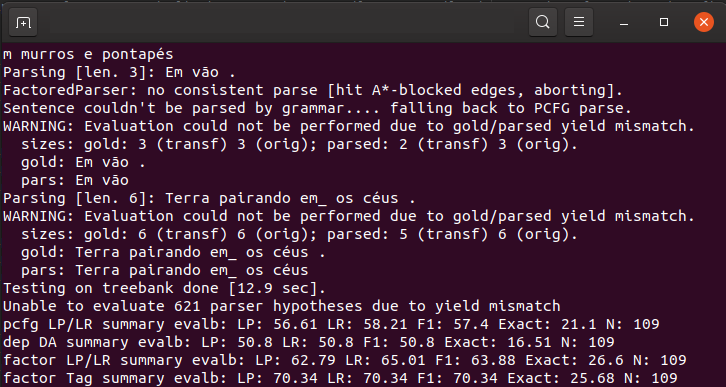
\includegraphics[width=100mm,scale=1.5]{imagens/cintil_training_error.png}
    \caption[Erro decorrente do mal posicionamento de pontuações na árvore do CINTIL]{Captura de tela de erro decorrente do mal posicionamento de pontuações na árvore do CINTIL, com relação ao formato PTB}
    \label{fig:cintil_training_error}
\end{figure}
\end{center}

% ------------------------------------------------------------------------------------------------
\subsection{Treinamento}
\label{subsec:treinamento_cintil}

Para fazer estas conversões, fizemos um \textit{script} disponível online\footnote{\url{ https://github.com/Fernandomn/treebank-transductor}}.

Com as \textit{tags} convertidas, foi feito o treinamento. O ato do treino é relativamente simples: deve-se, através do terminal do seu sistema, navegar até o diretório onde se encontra o \textit{stanford-parser.jar}, o arquivo que contém os \textit{parsers} do SP que utilizaremos. Estando no diretório correto, deve-se executar o comando \ref{lst:testeBasicoCintil}:

\begin{center}
\begin{lstlisting}[breaklines, caption={Execução de treinos do Stanford Parser para o CINTIL},label={lst:treinoBasicoCintil},language=Bash]
    java -cp ~/<diretorio de trabalho>/stanford-parser.jar -mx4g edu.stanford.nlp.parser.lexparser.LexicalizedParser -train ~/<diretorio do treebank>/tree-trad 1-1014 -saveToSerializedFile ~/<diretorio de armazenamento>/serialGrammarCINTIL -saveToTextFile ~/<diretorio de armazenamento>/textGrammarCINTIL
\end{lstlisting}
\end{center}

O código acima merece algumas explicações a parte, para quem não está familiarizado ao uso do SP pelo terminal.

\begin{center}
\begin{table}[h!]
    \centering
    \begin{tabular}{p{0.8\textwidth}}
        \begin{itemize}
            \item [-cp] \textit{ClassPath}. Indica o diretório onde se encontra a classe principal a ser executada
            \item [-mx4g] Quantidade de memória usada. No caso, 4 GB.
            \item [LexicalizedParser] \textit{Parser} utilizado, dentre os disponibilizados
            \item [-train] Treino. Logo em seguida, um diretório e a lista de arquivos a serem usados para treinar
            \item [-saveToSerializedFile] Salva o resultado do treino num arquivo binário, cujo diretório está indicado na sequência
            \item [-saveToTextFile] Salva o resultado do treino num arquivo de texto, cujo diretório está indicado na sequência
        \end{itemize}
    \end{tabular}
    \caption[Comandos para um treino simples do \textit{Stanford Parser}]{Comandos para um treino simples do \textit{Stanford Parser}, utilizando o terminal.}
    \label{tab:tab_treino_basico_cintil}
\end{table}
\end{center}

A Tabela \ref{tab:tab_treino_basico_cintil} mostra um fragmento das possibilidades de comandos a serem usados pela interface do terminal do SP. Note que usamos apenas 1014 arquivos nesta demonstração, que é um fração de 10\% dos arquivos / árvores do CINTIL disponíveis.

Para melhor verificação dos resultados, utilizamos o método de \textit{10-fold cross-validation}. Este método, como explicado por \citeonline{james2013introduction},
\begin{displayquote}
    \textquote{\textit{[\ldots] involves randomly dividing the set of observations into k groups, or folds, of approximately equal size. The first fold is treated as a validation set, and the method is fit on the remaining k -- 1 folds}}
    \footnote{\textquote{Esta abordagem envolve dividir aleatoriamente o conjunto de observações em k grupos, ou dobras, de tamanhos aproximadamente iguais. O primeiro grupo é tratado como conjunto de validação, e o método se encaixa nos k -- 1 grupos restantes}. Tradução própria.}.
\end{displayquote}

No nosso caso, dividimos nosso \textit{corpora} em 10 partes de 1014 sentenças. Fizemos o treinamento com 9 partes, e o teste com a parte restante, alternando as partes escolhidas. Os resultados serão apresentados na conclusão.

Na sequência, foi executado o treinamento com as partes restantes. De maneira análoga, no mesmo diretório, foi utilizado o comando \ref{lst:testeBasicoCintil}:

\begin{center}
\begin{lstlisting}[breaklines, caption={Execução de testes do Stanford Parser para o CINTIL},label={lst:testeBasicoCintil},language=Bash]
    java -cp stanford-parser.jar -mx4g edu.stanford.nlp.parser.lexparser.LexicalizedParser -loadFromSerializedFile /home/fernando/projeto-final-parsers/serialized-files/serialGrammarCINTIL1 input/sentencas_teste_cintil.txt

\end{lstlisting}
\end{center}

Que também merece explicações, na Tabela \ref{tab:tab_teste_basico_cintil}:
\begin{center}
\begin{table}[h!]
    \centering
    \begin{tabular}{p{0.8\textwidth}}
        \begin{itemize}
            \item [-cp] \textit{ClassPath}. Indica o diretório onde se encontra a classe principal a ser executada
            \item [-mx4g] Quantidade de memória usada. No caso, 4 GB.
            \item [LexicalizedParser] \textit{Parser} utilizado, dentre os disponibilizados
            \item [-writeOutputFiles ] Indica que os testes imprimirão arquivos de saída, a serem definidos
            \item [-outputFilesDirectory] Define o diretório onde os arquivos de saída serão escritos. 
            \item [-loadFromSerializedFile] Carrega a gramática serializada, gerada na execução de treinamento anterior
            \item [-testTreebank] Diretório onde se encontra o treebank a ser usado para teste. Os números no formato $a-b$ indicam o primeiro e o último arquivo, respectivamente. Números no formato $a-b,c-d$ indicam dois blocos de arquivos. Atente para não usar o mesmo bloco dos treinos, ou o parser passará por \textit{overfitting}, e terá resultados enviesados.
        \end{itemize}
    \end{tabular}
    \caption[Comandos para um teste simples do Stanford Parser]{Comandos para um teste simples do Stanford Parser, utilizando o terminal.}
    \label{tab:tab_teste_basico_cintil}
\end{table}
\end{center}

O resultado total dos testes resultou na extensa Tabela \ref{tab:cintil_result_full}, que pode ser vista nos apêndices. E os comentários dos resultados pode ser encontrado em \ref{resultados_cintil}.
\section{Treinando o Stanford Parser sobre Bosque}
\label{sec:treinando_sp_bosque}

Como já visto, o Bosque é disponibilizado em duas variantes, português brasileiro (BR) e português europeu (PT). Este trabalho foi feito considerando ambas, porém focando na variante brasileira.

Como descrito em \ref{subsec:florestasintatica}, cada nó das árvores do Bosque são muito ricos em informação sintática. Como descrito em \ref{subsec:PennTB}, o PTB é \textquote{pobre}, se posto em comparação. Coube, então, fazer a remoção das outras características, mantendo apenas as \textit{tags} de \textquote{forma}, que equivalem às \textit{POS tags}.

Uma dificuldade, é que o arquivo de entrada está no formato ISO-8859. Ao ser convertido para o formato de texto aceito pelo SP (UTF-8), vários caracteres especiais, como letras acentuadas, se perdem. Foi necessário fazer a conversão do arquivo fonte, antes de realizar as operações de transdução. O comando utilizado pode ser visto em \ref{lst:convertUTF8}:
\begin{center}
    \begin{lstlisting}[breaklines, caption={Conversão de arquivo ISO para UTF-8},label={lst:convertUTF8},language=Bash]
    $ iconv -f ISO-8859-1  Bosque_CF_8.0.PennTreebank.ptb -t UTF-8 -o Bosque_CF_PTB.txt
\end{lstlisting}

\end{center}
Assim como o CINTIL, parte importante do nosso trabalho foi transduzir as \textit{tags} do BOSQUE para o padrão PTB. Isso implicou em decisões que serão apresentadas na Tabela \ref{tab:tab_bosque}:

\begin{center}
    \begin{longtable}{|p{0.1\linewidth}|p{0.2\linewidth}|p{0.15\linewidth}|p{0.15\linewidth}|p{0.3\linewidth}|}
\caption{Tabela de conversão: BOSQUE para PTB}\\
\hline
\textbf{Tag Original (Português)} & \textbf{Nome da Tag} & \textbf{Tag Convertida} & \textbf{Ocorrências} & \textbf{Observações}\\
\hline
\endfirsthead
\multicolumn{5}{c}%
{\tablename\ \thetable\ -- \textit{Continuação da página anterior}} \\
\hline
\textbf{Tag Original (Português)} & \textbf{Nome da Tag} & \textbf{Tag Convertida} & \textbf{Ocorrências} & \textbf{Observações} \\
\hline
\endhead
\hline \multicolumn{5}{r}{\textit{Continua na próxima página}} \\
\endfoot
\hline
\endlastfoot
    acl & Forma Oracional averbais & ?? & 277 & Não possui conversão direta. Melhor explicado em \ref{subsec:tag_acl}\\
    adj & adjectivos & JJ & 3484 & \\
    adjp & Sintagma adjectivais & ADJP & 3367 & \\
    adv & advérbios & RB & 3052 & \\
    advp & Sintagma adverbiais & ADVP & 2288 & \\
    art & artigos & DT & 10742 & \\
    conj-c & conjunções coordenativa & CC & 1723 & Explicado na sessão \ref{subsec:cu}\\
    conj-s & conjunções subordinativa & IN & 798 & \\
    cu & sintagma evidenciador de relação de coordenação & \_CU\_ & 1744 & Será explicado na sessão \ref{subsec:cu}\\
    ec & prefixos & \_EC\_ & 80 & Será explicado na sessão \ref{subsec:sec_ec}\\
    fcl & Forma Oracional Finita & VP & 6040 & Sentenças onde os verbos não estão no infinitivo. Sintagma verbal\\
    icl & Forma Oracional não finita & VP & 1827 & Sentenças onde os veros estão conjugados. Sintagma Verbal\\
    intj & interjeições & UH & 22 & \\
    n & substantivos & NN & 15724 & \\
    n-adj & substantivos / adjectivos & NN & 174 & Pesquisa mostrou que são todas as ocorrências são substantivos\\
    np & Sintagma nominais & NP & 22981 & \\
    num & numeral & CD & 1625 & \\
    pp & Sintagma preposicionais & PP & 11576 & \\
    pron-det & pronomes determinativos & DT & 1580 & Pelo \citeonline{posPTBguidelines}, \textquote{\textit{This category includes [\ldots] the indefinite determiners \textit{another}, \textit{any}, \textit{some}, \textit{each}, \textit{either} [\ldots], \textit{neither} [\ldots], \textit{that}, \textit{these}, \textit{this} and \textit{those} [\ldots]}}. No português, também, por \citeonline[p88]{mioto2013novo} \textquote{[\ldots] DP pode ter seu núcleo D preenchido por um item que tenha valor de determinante como artigos, demonstrativos e interrogativos[\ldots]}\\
    pron-indp & pronomes independentes & PRP & 1001 & PTB considera 4 tipos de pronomes: os pessoais, possessivos, wh-possessivos e wh-pessoais. Decidimos manter a marcação de pronomes pessoais. Isso é reforçado pela própria descrição de \citeonline{freitas2007biblia}, \textquote{pronome independente (com comportamento semelhante ao nome)}\\
    pron-pers & pronomes pessoais  & PRP & 891 & \\
    prop & nomes próprios & NNP & 4575 & \\
    prp & preposições & IN & 11694 & \\
    sq & Sintagma sequências discursivas & S & 56 & Marcador de Sentença\\
    v-fin & verbos finitos & VBP & 6167 & Verbos conjugados\\
    v-ger & verbos gerúndios & VBG & 328 & \\
    v-inf & verbos infinitivos & VB & 1684 & \\
    v-pcp & verbos particípios & VBN & 1577 & \\
    vp & Sintagma verbais & VP & 8103 & \\
    x & <desconhecido> & VB & 552 & Explicado na sessão \ref{subsec:sec_x}

\label{tab:tab_bosque}

\end{longtable}
\end{center}

Primeiramente, transduzimos todas as \textit{tags} em sequência, mantendo a estrutura das árvores originais. Notamos, então, que para além da tradução de \textit{tags}, algumas particularidades entre \textit{treebanks} precisou de uma análise distinta, para maior consistência. Tais procedimentos são descritos a seguir.
% ------------------------------------------------------------------------------------------------
\subsection{Problemas com EC (Prefixos)}
\label{subsec:sec_ec}

% Palavras marcadas com \textquote{ec}, tag de prefixos, são (como o nome indica) prefixos.
Prefixos são marcados com a \textit{tag} \textquote{ec}.
No caso em específico, o prefixo (ou morfema prefixal) que recebem tais marcações são aqueles ligados à palavra por hifens, como na Figura \ref{fig:bosque_2166}:

\begin{center}
    \begin{figure}[!ht]
    % \centering
    % \includegraphics{}
    \begin{center}
        \begin{minipage}{10cm}
            \begin{tabbing}
                \=\ldots\=\+\\
                \>(>N:ec:ex-:: ex-)\\
                \>(H:n:jogador:M\_P::: jogadores)\-\\
                \>\ldots
            \end{tabbing}
        \end{minipage}
    \end{center}
    \caption[Demonstração do uso de \textquote{ec} no Bosque]{Trecho da sentença CF515-1, do Bosque: \textquote{Ex-jogadores elogiam os colunistas Telé e Cruyff}. Demonstração da aplicação da \textit{tag} \textquote{ec}.}
    \label{fig:bosque_2166}
\end{figure}
\end{center}

O PTB não prevê situações como estas. Pelo contrário, como podemos ver no guia de marcações do PTB \cite[p~315]{bracketing_ptb}, tal estrutura é ignorada. Podemos ler a respeito do uso de hifens em (\textit{\Ibidem[p~58]{bracketing_ptb}}), mas tal trecho não nos informa sobre o tratamento de prefixos. Recolhendo um exemplo do próprio corpus, analisemos a Figura \ref{fig:ptb_0012}.

\begin{center}
    \begin{figure}[!h]
    % \includegraphics{}
    % wsj\_0012: In mid-October, Time magazine lowered its guaranteed [\ldots]\\\\
    \centering
    \begin{minipage}{10cm}
        \ldots
        \begin{tabbing}
        \centering
            \=( (S (S \=\+\\
            \>(PP-TMP In\=\+\\
            \>(NP \textbf{mid-October})\-\\
            \>),\\
            \>(NP-SBJ-1 Time magazine)\\
            \>(VP lowered\\
        \end{tabbing}
        \ldots
    \end{minipage}
    
    \caption[Fragmento da sentença wsj\_0012, do PTB, sobre aplicação de prefixos]{Fragmento da sentença wsj\_0012, do PTB: \textquote{\textit{In mid-October, Time magazine lowered its guaranteed circulation rate base for 1990 while not increasing ad page rates; with a lower circulation base, Time's ad rate will be effectively 7.5\% higher per subscriber; a full page in Time costs about \$120,000.}}}
    \label{fig:ptb_0012}
\end{figure}
\end{center}

A flexão \textquote{\textit{mid-October}} é representada, sozinha, como um sintagma nominal (\textit{noun phrase}). Portanto, fez-se necessário a criação de uma sub-tarefa que removesse tais \textit{tags}, e que a estrutura fosse refeita, de modo a seguir os padrões do PTB.

% ------------------------------------------------------------------------------------------------
\subsection{PROBLEMAS COM \% (PORCENTAGEM)}
\label{subsec:percent}
% Mais um caso interessante de distinção Bosque / PTB. 
O tratamento de porcentagem no Bosque é mais um caso interessante de sua diferença com o PTB.
Para o Bosque, o sinal de percentagem (\%) participa de um nó isolado marcado como substantivo, como na Figura \ref{fig:bosque_percent}. De acordo com a \cite[p~113-114]{afonso2006arvores}, este é um caso tratado como partitivo. \textquote{Por expressões partitivas entende-se tipos de expressões de quantificação que designam partes de um todo}, e \textquote{Geralmente a unidade dividida em partes (expressa em expressões partitivas) é de natureza nominal ou são quantificadores}. Para o PTB, \textquote{\textit{Percent is simply a flat NP, whether or not it is written with a space}}, como pode ser observado na Figura \ref{fig:ptb_percent_guide}.
\begin{center}
    \begin{figure}[!h]
    % \includegraphics{}
    CF77-4 \textquote{Cerca de 72\textbf{\%} dos empresários da construção querem que o próprio setor negocie a conversão dos contratos para a URV, enquanto 28\% desejam que o governo estabeleça as regras.}\\
    \centering
    \begin{minipage}{10cm}
        A1\\
        STA:fcl\\
        =SUBJ:np\\
        ==>N:ap\\
        ===>A:adv('cerca\_de')  Cerca\_de\\
        ===H:num('72' <card> M P)  72\\
        ==\textbf{H:n('\%' M P)  \%}\\
        ==N<:pp\\
        ===H:prp('de' <sam->)  de\\
        ===P<:np\\
        ====>N:art('o' <-sam> <artd> M P)  os\\
        ====H:n('empresário' M P)  empresários\\    
        \ldots
    \end{minipage}
    \caption[Exemplo de marcação de porcentagem pelo Bosque]{Exemplo de marcação de porcentagem pelo Bosque, formato Árvores Deitadas. Adaptado de \cite[p~115]{afonso2006arvores}}
    \label{fig:bosque_percent}
\end{figure}
\end{center}

% Tal estrutura foi reproduzida mas, não pudemos precisar o motivo, o SP não aceita as estruturas convertidas por nós que possuam \%. Resolvemos, portanto, remover tais sentenças da análise.
A estrutura foi reproduzida pelo \textit{script} desenvolvido, mas o SP não foi capaz de processá-lo. Num momento futuro, será investigado o motivo de tal comportamento. A priori, fez-se necessário descartar tais sentenças. Isso dá um total de 149 sentenças, aprox. 3,5\% do \textit{dataset} completo.
\begin{center}
    \begin{figure}[!ht]
    % \includegraphics{}
    \centering
    \begin{minipage}{5cm}
        (NP 15 \textbf{percent})\\
        (NP 15 \textbf{per cent})\\
        (NP 8.45 \textbf{\%})
    \end{minipage}
    \caption[Exemplo de representação de porcentagem para o PTB]{Exemplo de representação de porcentagem para o PTB. Adaptado de \citeonline[p~308]{bracketing_ptb} }
    \label{fig:ptb_percent_guide}
\end{figure}
\end{center}
% ------------------------------------------------------------------------------------------------
\subsection{PROBLEMAS COM PONTUAÇÃO}
\label{subsec:bosque_point}

O Bosque tem uma política de tratamento de símbolos mais parecida com a do PTB. Porém, envolve uma pluralidade maior de possíveis sinais, além de usar sinais não convencionais, como \guillemotleft, por exemplo. A Tabela \ref{tab:bosque_points} mostra os símbolos utilizados, além de suas respectivas frequências de ocorrência no \textit{treebank}.
\begin{center}
    \begin{table}[!h]
    \centering
    \begin{tabular}{|l|r|l|r|}
        \hline
        Simbolo & Frequência & Simbolo & Frequência\\
        \hline
        !   &    59     &   ;   &    208\\
        '   &    45     &   ?   &    78\\
        ,   &    4432   &   [  &    1\\
        -   &    1      &   ]  &    1\\
        - -  &    103    &   \{  &    453\\
        .   &    3396   &   \}  &    456\\
        \ldots & 17     &   \guillemotleft & 707\\
        $\backslash$  &   3       &   \guillemotright & 703\\
        \hline
    \end{tabular}
    \caption{Tabela de símbolos presentes no CETEMFolha, e suas respectivas frequências de aparecimento.}
    \label{tab:bosque_points}
\end{table}
\end{center}

O Bosque tem uma descrição extensa sobre o posicionamento de pontuações. Por \cite[p~27]{afonso2006arvores}, \textquote{A pontuação não tem qualquer informação morfossintática associada, embora possa ser um indicador de estatuto sintáctico, estando tão só indentada}. A priori é uma política muito semelhante à do PTB, como vimos em \ref{subsec:cintil-pnt}.

Existem três casos distintos a serem considerados na hora de posicionar pontuações: inicio, final, e dentro de frases. Para pontuações em inicio e fim de frase, \cite[p~28]{afonso2006arvores} \textquote{indentação ao mais alto nível de constituinte imediatamente abaixo da raiz}. Para pontuações dentro de frase, temos dois casos, como delimitadores, e como separadores. Para delimitadores, 
\begin{quote}
    \textquote{[É a] pontuação que delimita trechos de texto colocada ao mesmo nível dos nós mais altos correspondentes a esse trecho, quer seja um nó não terminal ou o um nó terminal. Estes casos incluem os seguintes tipos de pontuação: aspas, parênteses, vírgulas, travessões}.
\end{quote}
Para separadores, \cite[p~30]{afonso2006arvores} \textquote{[É a] pontuação que separa trechos, colocada ao mesmo nível do trecho que se inicia a partir da pontuação que o separa do trecho anterior. Incluem-se neste caso a vírgula, ponto e vírgula, dois pontos, travessão}. Por fim, \cite[p~33]{afonso2006arvores} 
\begin{quote}
    \textquote{A pontuação final permite identificar a frase como constituindo um elemento comunicativo [\ldots], e por isso é considerada como fazendo parte integrante da frase. Por vezes, uma \textquote{frase analisada} corresponde a uma sequência de \textquote{frases} como funções principais (STA, QUE, EXC, e UTT).}
\end{quote}

% Todo símbolo, no Bosque, está envolto em parênteses, e posicionado de maneira semelhante à utilizada no PTB. Foi necessário, portanto, apenas converter os sinais relevantes (chaves \textquote{\{}, por exemplo), e posicioná-los no mesmo local. 
As sentenças geradas pelo nosso \textit{script} não eram processadas corretamente pelo SP, que acusa erro semelhante ao citado em \ref{subsec:cintil-pnt}, como pode ser visto na Figura \ref{fig:bosque_erro_mismatch}. Assim como no CINTIL, removemos os símbolos das sentenças, para permitir a continuidade dos testes.
\begin{center}
    \begin{figure}[!h]
    \centering
    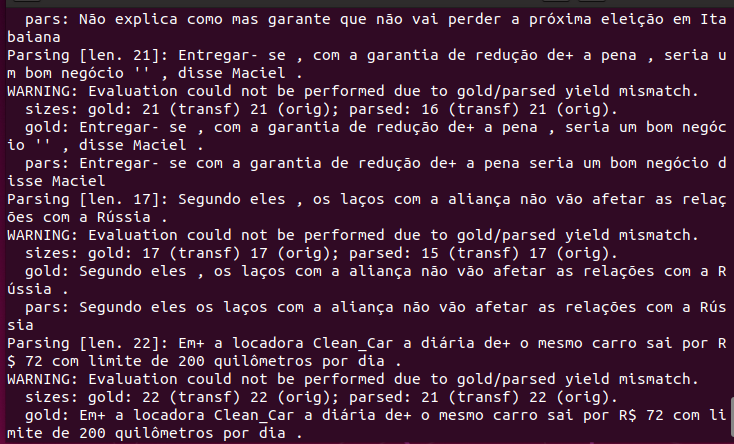
\includegraphics[width=.8\textwidth,scale=1.5]{imagens/erro_mismatch.png}
    \caption[Erro de não casamento (\textit{mismatch}) entre árvores]{Erro de não casamento (\textit{mismatch}) entre árvores ao executar o SP sobre o Bosque pré-treinado.}
    \label{fig:bosque_erro_mismatch}
\end{figure}
\end{center}
% ------------------------------------------------------------------------------------------------
\subsection{Problemas com CU (Coordenação)}
\label{subsec:cu}
Coordenação é uma das \textit{tags} mais problemáticas do BOSQUE. Como destacam \citeonline[p~4]{Wing2006Adaptation}:
\begin{quote}
    \textquote{\textit{Conjoined clauses in the native Floresta are of type CU, regardless of the type of constituents being conjoined. This causes grammars learned from the treebank to make errors such as conflating noun phrase conjunctions and sentential conjunctions}}.
    \footnote{\textquote{Cláusulas conjuntivas no Floresta nativo são do tipo CU, independentemente do tipo de constituinte conjunto. Isso faz com que a gramática aprendida do treebank cometa erros como confundir conjunções de sintagmas nominais e conjunções sentenciais}. Tradução própria.}.
\end{quote}

O PTB tem suas próprias regras para determinar a estrutura de coordenações, reservando o Capítulo 7 de seu \textit{Bracketing Guidelines}\footnote{Manual de Agrupamento} \cite[p~117]{bracketing_ptb}. Seguindo tais regras, num primeiro momento de tradução, apenas marcamos as coordenações com a \textit{tag} auxiliar \_CU\_. Depois, fizemos uma nova verificação, reconhecendo as sentenças onde essa marca aparece.
\begin{center}
    \begin{figure}[!h]
    \centering
    \begin{minipage}{10cm}
        \begin{tabbing}
            \=(\textbf{H:cu}\=\+ \\
            \>    (CJT:\=np \+\\
            \>        (H:n:saúde:F\_S::anr\_np-def: saúde))\-\\
            \>    \=(CO:conj-c:e:::: e)\\
            \>    (CJT:\=np \+\\
            \>        (H:n:educação:F\_S::np-idf: educação)))))))
        \end{tabbing}
    \end{minipage}
    % \includegraphics{}
    \caption[Exemplo de uso do sintagma evidenciador de coordenação no Bosque]{Exemplo de uso do sintagma evidenciador de coordenação no Bosque. Fragmento da sentença CF5-2}
    \label{fig:bosque_exemplo_cu}
\end{figure}
\end{center}

Já citamos, em \ref{subsec-cintil-conj}, que o PTB lida com a coordenação de basicamente três formas: palavras simples, palavras múltiplas e conjunções descontínuas. A \textit{tag} \textit{cu} define o sintagma que encabeça a coordenação. Isto pode ser melhor visto na Figura \ref{fig:bosque_exemplo_cu}. Isto facilita o procedimento pois, deve-se então verificar se os sintagmas filhos possuem a mesma \textit{tag}, e se são nós terminais ou não-terminais. Sendo terminais, devem ser impressos numa estrutura achatada (\textit{flat structure}). Sendo não-terminais, de mesma categoria, a \textit{tag} cu deve ser convertida para uma \textit{tag} equivalente. Sendo sintagmas de categorias distintas, cu é convertido para UCP (\textit{Unlike Coordinated Phrase}\footnote{\textquote{Sintagma Coordenado Diferente}. Tradução própria.}).
\begin{center}
    \begin{figure}[!h]
    \centering
    \begin{minipage}{10cm}
        CF766-6 E o Brasil?
        \begin{tabbing}
            \=(FRASE\=  CF766-6 (QUE:np (\textbf{CO:conj-c:e:: E})\+\\
            \>    (>N:art:o:M\_S::artd: o)\\
            \>    (H:prop:Brasil:M\_S::: Brasil)\\
            \>    (?)))\\
        \end{tabbing}
    \end{minipage}
    % \includegraphics{}
    \caption[Exemplo árvore onde palavra marcada por conj-c não implica em conjunção entre sentenças]{Exemplo árvore onde palavra marcada por conj-c (conjunção coordenativa) não implica em conjunção entre sentenças}
    \label{fig:bosque_exemplo_conj-c}
\end{figure}
\end{center}

Tem-se, também, que tomar cuidado com os casos de palavras simples, em \textit{flat structure}. Por dois motivos: primeiro, não necessariamente uma palavra que, no Bosque, é marcada por conj-c (conjunção coordenativa), será um indicador de conjunção, efetivamente. Exemplo na sentença CF766-6, Figura \ref{fig:bosque_exemplo_conj-c}. Nesses casos, a palavra deve ser marcada com a \textit{tag} CC para o PTB. O segundo problema é a correta escrita da \textit{flat structure}. O \cite[p~117]{bracketing_ptb}  mostra alguns exemplos possíveis. Empiricamente, notamos que a forma correta deve ser como na Figura \ref{fig:bosque_exemplo_flat}, ou seja, o valor pós-conjunção deve ser destacado num novo sintagma.
\begin{center}
    \begin{figure}[!h]
    \centering
    \begin{minipage}{10cm}
        \begin{tabbing}
            \=(VP \=\+\\
            \>    (IN \=porque)\+\\
            \>        (VP \=\+\\
            \>            (VBP tem)\-\\
            \>        )\\
            \>        (NP \=\+\\
            \>            (NN gente)\-\\
            \>        )\\
            \>        (VP \=\textbf{comprando e}\+\\
            \>            (\textbf{VBG vendendo})))
        \end{tabbing}
    \end{minipage}
    % \includegraphics{}
    \caption[Exemplo de como coordenações \textit{single word} devem se comportar]{Exemplo de como coordenações \textit{single word} devem se comportar. Fragmento da conversão da sentença \textit{CF400-2 Diretor do Banco Central não acredita que o real esteja valorizado porque \guillemotleft tem gente comprando e vendendo\guillemotright}}
    \label{fig:bosque_exemplo_flat}
\end{figure}


\end{center}
% ------------------------------------------------------------------------------------------------
\subsection{O par \textbf{x} e \textbf{X}}
\label{subsec:sec_x}
Ainda há, no \textit{corpus}, o par de \textit{tags}, X e x. X é uma \textit{tag} do tipo função, e x uma \textit{POS tag}. Na Bíblia Florestal (\cite{freitas2007biblia}), não há uma descrição formal para ambas. Apenas notou-se que nunca aparecem em par, mas quase sempre próximas. Num primeiro momento, a solução foi ignorar este par, descartando toda sentença / árvore em que aparecem. Mas uma revisão mostrou que seria uma grande perda desprezá-los, e isso nos levou a uma série de desdobramentos interessantes.
\begin{center}
    \begin{table}[!h]
    \centering
    \begin{tabular}{|l|r|l|r|}
    \hline
        X:adv   &   1   &   CJT:x   &   480\\
        X:cu    &   22  &   EXC:x   &   1\\
        X:np    &   3   &   N<:x    &   18\\
        X:pp    &   130 &   P<:x    &   1\\
        	    &       &   PIV:x   &   3\\
        	    &	    &   UTT:x   &   2\\
        \hline
    \end{tabular}
    \caption{Pares possíveis para as tags X, e frequência de aparecimento no CETEMFolha}
    \label{tab:tag_X}
\end{table}
\end{center}

Na Tabela \ref{tab:tag_X}, mostramos quais as ocorrências das \textit{tags} X e x, em conjunto com seus possíveis pares (ou seja, \textquote{$(F:x)$ e $(X:f)$}, sendo \textit{f} e \textit{F} \textit{tags} quaisquer). Pode-se notar que, por mais que ambas sejam casadas com diversas etiquetas, no geral se associam à \textit{tags} de conjunção. Uma hipótese, então, é:
\begin{quote}
	X e x são \textit{tags} coringas. Elas ocupam o espaço da Função ou da Forma (respectivamente) quando a informação realmente relevante é apenas o seu par. 
\end{quote}

Isto gera um problema. Como descrito em \ref{subsec:florestasintatica}, todo nó tem pelo menos o par F:f, e como foi dito no começo da seção, deu-se preferência às \textit{tags} \textit{forma} (por serem equivalentes às \textit{POS tags}) em detrimento às outras. As \textit{tags} x nos forçam a voltar a olhar para as \textit{tags} irmãs. Ou seja, nos casos em que o nó possui uma \textit{tag} x, F informará o valor a ser convertido. As \textit{tags} F, então, necessitam de uma nova tabela, que pode ser vista na Tabela \ref{tab:bosque_func_edit}.
\begin{center}
    \begin{longtable}{|p{0.1\linewidth}|p{0.2\linewidth}|p{0.15\linewidth}|p{0.15\linewidth}|p{0.3\linewidth}|}
\caption{Tabela de conversão: BOSQUE para PTB (Funções relevantes)}\\
\hline
\textbf{Tag Original (Português)} & \textbf{Nome da Tag} & \textbf{Tag Convertida} & \textbf{Ocorrências} & \textbf{Observações}\\
\hline
\endfirsthead
\multicolumn{5}{c}%
{\tablename\ \thetable\ -- \textit{Continuação da página anterior}} \\
\hline
\textbf{Tag Original (Português)} & \textbf{Nome da Tag} & \textbf{Tag Convertida} & \textbf{Ocorrências} & \textbf{Observações} \\
\hline
\endhead
\hline \multicolumn{5}{r}{\textit{Continua na próxima página}} \\
\endfoot
\hline
\endlastfoot
    \textgreater A & dependente em adjp ou advp (antecede o núcleo) & \textgreater A & 371 & Explicado em \ref{subsec:bosque_a} \\
    A\textless & dependente em adjp ou advp (segue o núcleo) & A\textless & 272 & Explicado em \ref{subsec:bosque_a} \\
    ACC & objecto directo (incluindo alguns tipos de se) & depende da \textit{form\_tag} & 4315 & Explicado em \ref{subsec:tag_acl}\\
    ADVL & adjunto adverbial & depende da form & 6032 & Explicado em \ref{subsec:tag_acl}\\
    CJT & elemento conjunto & \_CJT\_ & 3945 & Explicado em \ref{subsec:CJT}\\
    EXC & enunciado exclamativo & S & 36 & \\
    H & núcleo & depende da form & 40148 & \\
    KOMP\textless  & complemento comparativo & \_KOMP\_ & 40 & Explicado em \ref{subsec:tag_komp}\\
    \textgreater N & adjunto adnominal (antecede o núcleo) & NP & 14009 & Dobra do NP por adjunto, como visto em \citeonline[p~67]{mioto2013novo}
    \footnote{\citeonline[p~67]{mioto2013novo} descreve a dobra de sintagmas para adjuntos.
    \begin{quote}
        \textquote{[\ldots] existem ainda sintagmas que são licensiados numa sentençça sem serem complemento ou especificador de um núcleo. São os chamados \textbf{adjuntos}. [\ldots] Um adjunto [\ldots] é um sintagma que está apenas contido na projeção máxima de um núcleo. [\ldots] A representação do adjunto sempre implica a duplicação da categoria com a qual ele está relacionado. Desta forma, o adjunto vai ser dominado apenas pelo segmento de cima da categoria duplicada.}
    \end{quote}}
    \\
    N< & adjunto adnominal (segue o núcleo) & NP & 9208 & Dobra do NP por adjunto, como visto em \citeonline[p~67]{mioto2013novo}\\
    OC & predicativo do objeto & depende da form & 102 & Explicado em \ref{subsec:tag_acl}\\
    \textgreater P & dependente da preposição & PP & 71 & Por observação, e por \citeonline[p~67]{mioto2013novo}\\
    P & predicador & VP & 8053 & Pela \citeonline[p~60]{afonso2006arvores}, O predicador é sempre de natureza verbal e, por isso, pode exibir apenas formas verbais\\
    P< & argumento de preposição & PP & 11574 & Por observação, e por \citeonline[p~67]{mioto2013novo}\\
    PIV & objecto preposicional & PP & 1097 & \\
    QUE & enunciado interrogativo & S & 64 & \\
    SC & predicativo do sujeito & VP & 1254 & \\
    STA & enunciado declarativo & S & 3683 & \\
    UTT & enunciado & S & 468 &

\label{tab:bosque_func_edit}

\end{longtable}
\end{center}

A Tabela \ref{tab:bosque_func_edit} é um fragmento da Tabela \ref{tab:bosque_func_full}, que pode ser encontrada nos apêndices. Esta última possui, efetivamente, todas as \textit{tags} de função, seus nomes, possíveis conversões etc. Diversas delas não serão utilizadas neste trabalho, portanto não necessitam ser abordadas nesta seção.

Isso nos leva a novas questões. Nem todas as \textit{tags} de função são explícitas quanto ao sintagma que elas definem. Ou seja, uma informação de sintagma precisa seria obtida pela \textit{tag} $f$, que no caso é $x$, que não tem valor sintagmático, e o PTB não prevê sintagmas não marcados, ou etiquetas coringa. Vamos verificar essas funções nas próximas sessões, e as estratégias utilizadas para resolver tais problemas.

% ------------------------------------------------------------------------------------------------
\subsection{PROBLEMAS COM >A e A<}
\label{subsec:bosque_a}

Vemos em \cite[p~13]{afonso2006arvores}
% \begin{quote}
    \textquote{A indicação de \textquote{>} e \textquote{<} presentes nas funções acima, reflectem a posição do dependente face ao núcleo, como setas direccionadas para o núcleo cuja natureza está indicada por letras maiúsculas}. 
% \end{quote}
Vemos também que 
% \begin{quote}
    \textquote{Por outro lado, >A significa que o dependente aponta para o núcleo de natureza adjectival ou adverbial (\textquote{A}) que se encontra à direita do dependente (\textquote{>})}.
% \end{quote}

A possível ambiguidade da sentença anterior é resolvida em \cite[p~58]{afonso2006arvores}, no qual se lê \textquote{As mesmas etiquetas, A< e >A, como se pode constatar, estão presentes tanto nos sintagmas adjectivais como nos sintagmas adverbiais enquanto modificadoras de adjectivos ou advérbios}. Ou seja, para a correta conversão de >A (por exemplo) para ADVP, ou ADJP, é necessário olhar o nó irmão, e verificar o seu núcleo. Este sendo adjetivo ou sintagma adjetival, >A se torna ADVP, e análogo para advérbios. Mas o que fazer em casos como da sentença CF761-3 (Figura \ref{fig:bosque_a_seta_errado}), em que o nó irmão de >A é um advérbio, mas o núcleo do sintagma é adjetivo? 
\begin{center}
    \begin{figure}[!h]
    \centering
    \begin{minipage}{10cm}
        \ldots
        \begin{tabbing}
            \=(SC:\=adjp \+\\
            \>    (\textbf{>A}:\=x (X:pp\+\\ 
            \>          (H:prp:de:::: de)\\
            \>          (P<:\=np \+\\
            \>            (>N:num:30:M\_P::card: 30)\\
            \>            (H:n:\%:M\_P::anr\_np-count:anr\_np-def: \%)))\-\\
            \>        (X:\=pp \+\\
            \>          (H:prp:a:::: a)\\
            \>          (P<:\=np \+\\
            \>            (>N:num:40:M\_P::card: 40)\\
            \>            (H:n:\%:M\_P::anr\_np-count:anr\_np-def: \%))))\-\-\-\\
            \>    (\textbf{>A:adv}:mais:\_::KOMP:quant: mais)\\
            \>    (\textbf{H:adj}:rápido:F\_P::: rápidas)\\
            \>    (KOMP<:acl \\
        \end{tabbing}
        \ldots
    \end{minipage}
    % \includegraphics{}
    \caption[Exemplo de estrutura ambígua de >A]{Exemplo de estrutura ambígua de >A. Fragmento da árvore da sentença CF761-3 \textquote{As novas impressoras a laser da HP vêm com um novo padrão de velocidade 12 páginas por minuto (ppm) e são de 30\% a 40\% mais rápidas que as da geração anterior}.}
    \label{fig:bosque_a_seta_errado}
\end{figure}

\end{center}

Para este trabalho, os nós não conservam as informações de função, apenas de forma. Assim sendo, >A será transduzido de acordo com o primeiro nó válido na direção indicada por > ou <.
% ------------------------------------------------------------------------------------------------
\subsection{PROBLEMAS COM CJT (Conjunção)}
\label{subsec:CJT}
Ainda sobre sintagmas evidenciadores da relação de coordenação (visto em \ref{subsec:cu}), \cite[p~20]{afonso2006arvores} descreve: 
\begin{quote}
    \textquote{A sua estrutura interna evidencia também a relação de coordenação: duas ou mais partes coordenadas como função e uma ou mais conjunções coordenativas, que podem ou não estar presentes. A forma de cada uma das partes coordenadas segue os princípios gerais dos sintagmas não verbais, isto é, dependendo da sua estrutura interna e em particular da função dos dependentes do núcleo do sintagma, ou dos sintagmas verbais}.
\end{quote}

As \textquote{partes coordenadas} citadas são nós cuja função é CJT. Como é melhor explorado em \cite[p~96]{afonso2006arvores} \textquote{nós dependentes daquele, terminais ou não terminais, ao mesmo nível que correspondem às partes coordenadas $(CJT: forma)$}.

Quando tal tipo de função ocorre para um nó, a solução de transdução costuma ser simples: basta utilizar o valor de forma. O problema, claro, é que estamos aqui justamente por nossa \textit{forma} ser \textquote{x}, a etiqueta \textquote{coringa}. Nestes casos, empiricamente, notou-se uma frequência alta de sentenças internas à $(CJT:x)$ que possuem valor sintático de sintagma verbal (VP). Portanto, decidimos que os casos $(CJT:x)$ seriam convertidos para VP.
\begin{center}
    \begin{table}[!h]
    \centering
    \begin{tabular}{|l|r|l|r|}
        \hline
        CJT\&ACC:np & 1 & CJT:fcl & 596\\
        CJT\&ADVL:pp & 3 & CJT:icl & 123\\
        CJT\&PASS:pp & 1 & CJT:n-adj & 12\\
        CJT\&PRED:adjp & 2 & CJT:np & 1990\\
        CJT:acl & 12 & CJT:pp & 392\\
        CJT:adjp & 288 & CJT:v-ger & 2\\
        CJT:advp & 24 & CJT:v-pcp & 22\\
        CJT:cu & 6 & CJT:x & 480\\
        \hline
    \end{tabular}
    \caption{Possíveis combinações de CJT.}
    \label{tab:bosque_CJT}
\end{table}
\end{center}

Podemos ver na Tabela \ref{tab:bosque_CJT} a frequência com quem CJT se pareia, e vemos nele uma certa \textit{tag} chamada acl. Na Tabela \ref{tab:tab_bosque} podemos ver que ela merece uma atenção especial. Dedicaremos um pouco mais de tempo à ela.
% ------------------------------------------------------------------------------------------------
\subsection{PROBLEMAS COM ACL (ORAÇÕES AVERBAIS)}
\label{subsec:tag_acl}
Vemos em \cite{freitas2007biblia}, \textquote{Finalmente, na oração averbal
\footnote{Note que, em \cite[p~12]{afonso2006arvores}, acl é grifada como \textquote{oração deverbal}}
\footnote{\textquote{the crawling chaos\ldots}. \citeonline{lovecraft1920nyarlathotep}}
, o verbo não está presente, mas normalmente estas orações são encabeçadas por uma conjunção subordinativa que indica a natureza oracional do período}. Ao passo que fcl e icl (orações finitas e não-finitas) podemos afirmar serem conversíveis para VP, acl nos obriga a fazer conversões para a forma de oração subordinada \cite[p~172]{bracketing_ptb}, porém também não de forma assertiva. Pois, como vemos na Tabela \ref{tab:bosque_acl}, acl pode se ligar a qualquer forma sintagmática, inclusive início de orações. Porém, observar a função costuma dar uma informação bastante definitiva, conversão que adotamos nos casos de ADVL:acl, EXC:acl, N<:acl, N<PRED:acl, QUE:acl, STA:acl, UTT:acl. Para casos como ACC:acl e OC:acl, tomamos opções arbitrárias: convertemos para NP. Faltam dois casos então, KOMP< e CJT (novamente).
\begin{center}
    \begin{table}[!ht]
    \centering
    \begin{tabular}{|l|r|l|r|}
        \hline
        ACC:acl     &   1   &   N<PRED:acl  &   6\\
        ADVL:acl    &   78  &   OC:acl  &   31\\
        CJT:acl     &   12  &   QUE:acl &   1\\
        EXC:acl     &   4   &  	SC:acl  &   15\\
        KOMP<:acl   &   44  &   STA:acl &   3\\
        N<:acl      &   40  &   UTT:acl &   63\\
        \hline
    \end{tabular}
    \caption{Possíveis combinações da \textit{tag} \textit{acl}, e frequência de ocorrência no CETEMFolha}
    \label{tab:bosque_acl}
\end{table}
\end{center}
% ------------------------------------------------------------------------------------------------
\subsection{PROBLEMAS COM KOMP< (COMPLEMENTOS)}
\label{subsec:tag_komp}
Esta etiqueta é definida, por \cite[p~57]{afonso2006arvores} como \textquote{KOMP<, segundo termo de uma oração comparativa ou oração consecutiva}. E em \cite[p~116]{afonso2006arvores}:
\begin{quote}
    \textquote{Em termos de representação em árvores, a particularidade é o segundo termo de comparação ser etiquetado com KOMP< (etiqueta de sintagma) ao mesmo nível de constituintes que o adjectivo ou advérbio e o seu dependente. [\ldots] KOMP< terá como forma \textquote{fcl}, no caso de o verbo principal estar expresso ou \textquote{acl}, no caso de o verbo principal estar omisso}.
\end{quote}

É reservado o Capítulo 22 do \cite[p~284]{bracketing_ptb} para o estudo de comparativos. Nele, vemos:
\begin{quote}
    \textquote{\textit{The than, that, or as is bracketed as either a PP or an SBAR, and a certain amount of variations exists in the choice of PP, or SBAR. SBAR is used when the rest of the than/that/as-phrase is a tensed sentence, or when it contains a subject. PP is in general when the rest of the than/that/as-phrase is a single constituent [\ldots]}}.
\end{quote}

Dois exemplos simples podem ser vistos na Figura \ref{fig:ptb_exemplo_comp}. Foi necessário, então, repetir tal comportamento na transdução.
\begin{center}
    \begin{figure}[!h]
    \centering
    \begin{minipage}{.3\linewidth}
        \ldots
        \begin{tabbing}
            \=(PP \=than/as\+\\
            \>    (xP rest of phrase))\\
            \>\\
        \end{tabbing}
        \begin{tabbing}
            \=(SBAR \=than/that/as\+\\
            \>    (S rest of phrase))\\
        \end{tabbing}
        \ldots
    \end{minipage}
    % \includegraphics{}
    \caption[Exemplos de configurações das sentenças comparativas no PTB]{Exemplos de configurações das sentenças comparativas no PTB. Adaptado de \cite[p~284]{bracketing_ptb}}
    \label{fig:ptb_exemplo_comp}
\end{figure}




\end{center}
% ------------------------------------------------------------------------------------------------
\subsection{PROBLEMAS COM CJT:acl}
\label{subsec:CJT_acl}
Definitivamente, a mais desafiadora das conversões. Sentenças averbais com valor de conjunção. Não existe uma forma precisa de converter este par. 

Notou-se também que observar os nós filhos, ou mesmo os pais, não nos dariam informações precisas que nos permitisse afirmar qual seria uma transdução interessante, que fosse reconhecível tanto por PTB como por SP. Ser arbitrário, e defini-lo como VP ou NP, por exemplo, causaria muitos problemas. Não restava muitas escolhas. Como trabalho futuro, caberá o estudo deste par. Por ora, decidiu-se transduzí-los para \textquote{S} (marcador de Sentença).
% ------------------------------------------------------------------------------------------------
\subsection{PROBLEMAS COM O BOSQUE}
\label{subsec:erros_bosque}
Dentre as dificuldades na transdução Bosque/PTB, alguns erros no \textit{dataset} merecem ser frisados. Como já dito, o Bosque originalmente é distribuído no formato Árvores Deitadas, mas possui uma distribuição em formato \textit{Penn Treebank}. A observação nos mostra que, na prática, apenas foram substituídos os símbolos de indentação pelos parênteses do PTB. 
% Nos apêndices, haverá uma lista completa os que foram detectados por nós. 
% Neste momento, serão destacados alguns casos.
Destacam-se alguns casos.

P.vp - Na sentença CF624-3, a separação de etiquetas está incorreta. Ao invés de estar escrito \textquote{P:vp}, está grifado \textquote{P.vp}, como visto na Figura \ref{fig:bosque_erro_pvp}.

\begin{center}
    \begin{figure}[!h]
    \centering
    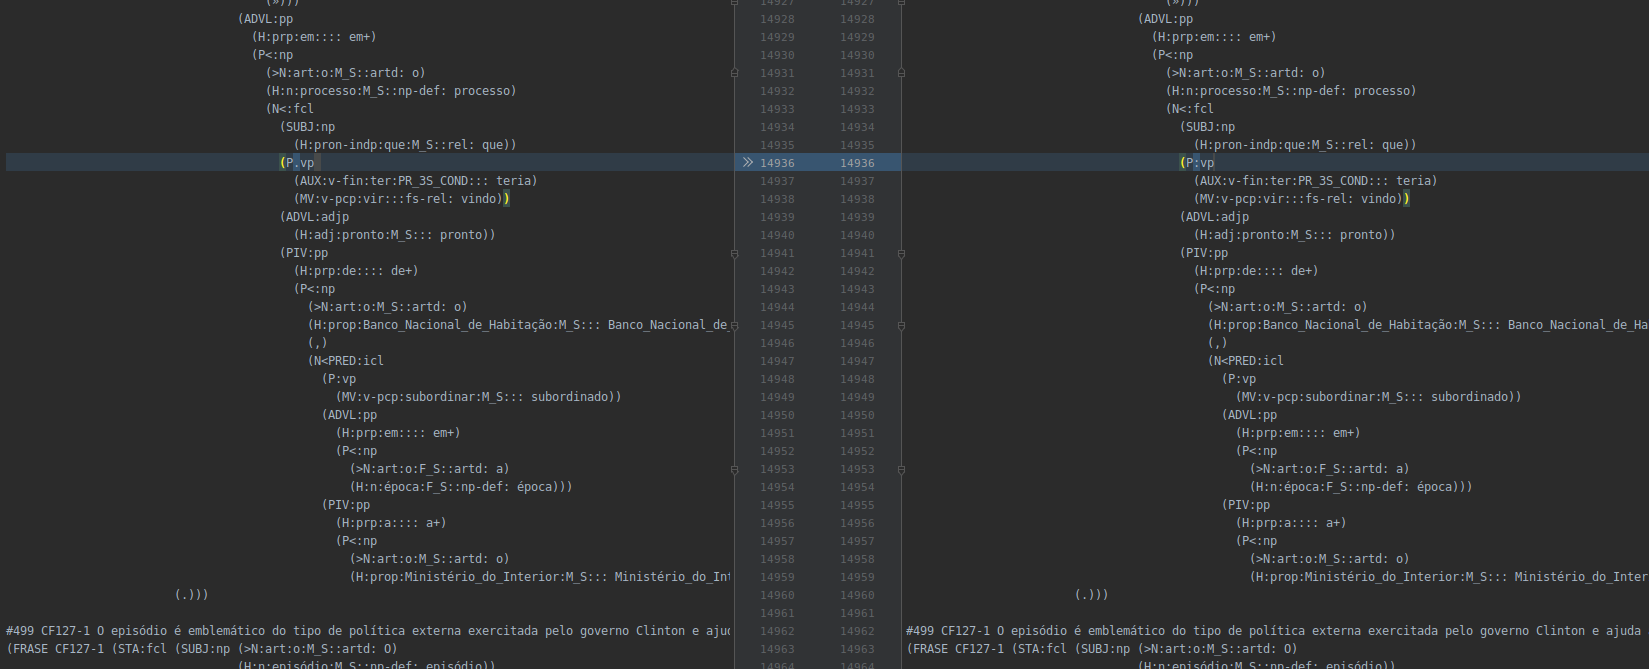
\includegraphics[width=\textwidth,scale=1.5]{imagens/erro_escrita_498.png}
    \caption[Erro na marcação do par P:vp]{Erro na marcação do par P:vp}
    \label{fig:bosque_erro_pvp}
\end{figure}
\end{center}

Nó terminal fechado de forma incorreta - Alguns nós que necessariamente são terminais (como determinantes, ou pronomes) ocorrem fechados de forma inconsistente. A correção foi necessária. A sentença CF624-3 contém um exemplo, que pode ser visto na Figura \ref{fig:bosque_erro_no_fechado_errado}.

\begin{center}
    \begin{figure}[!h]
    \centering
    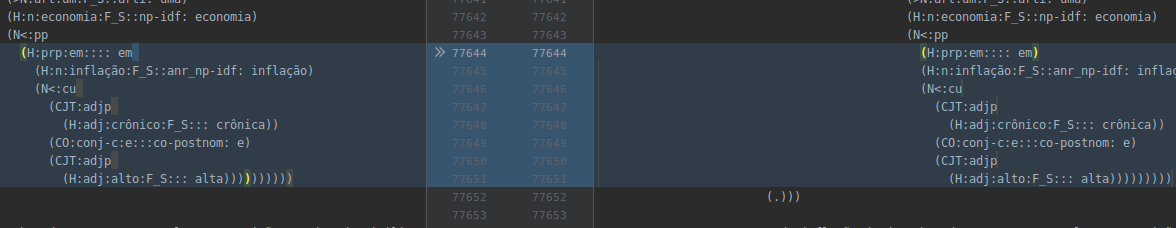
\includegraphics[width=\textwidth,scale=1.5]{imagens/erro_escrita_2626.png}
    \caption[Erro no fecho do nó H:prp]{Erro no fecho do nó H:prp}
    \label{fig:bosque_erro_no_fechado_errado}
\end{figure}
\end{center}

Símbolos marcados incorretamente - Bosque apresenta símbolos entre parentes, sem etiquetas. Isto ocorre em duas sentenças. Um exemplo é na sentença CF322-3, como pode ser visto na Figura \ref{fig:bosque_erro_simbolos}, com o parênteses abrindo para o símbolo, mas sem o fecho na sequência. 

\begin{center}
    \begin{figure}[!h]
    \centering
    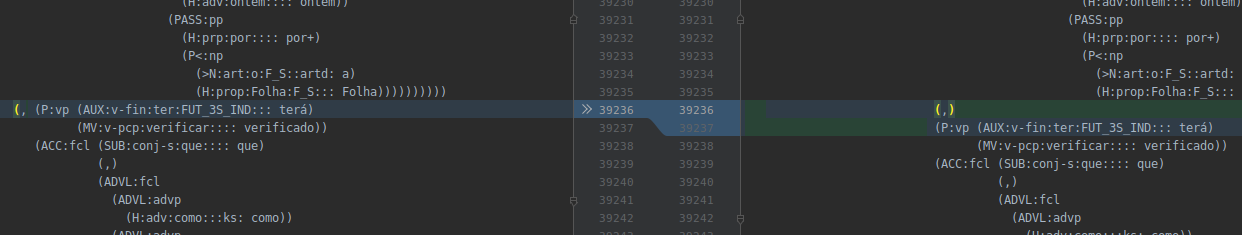
\includegraphics[width=\textwidth,scale=1.5]{imagens/erro_escrita_1340.png}
    \caption[Erro na marcação de símbolos]{Erro na marcação de símbolos}
    \label{fig:bosque_erro_simbolos}
\end{figure}
\end{center}

% ------------------------------------------------------------------------------------------------
\subsection{Treinamento}
\label{subsec:treinamento_bosque}
De modo análogo ao CINTIL, fizemos o treinamento baseado num comando simples, como visto no código \ref{lst:treinoBasicoBosque}
\begin{center}
    \begin{lstlisting}[breaklines, caption={Execução de treinos do Stanford Parser para o Bosque},label={lst:treinoBasicoBosque},language=Bash]
    java -cp stanford-parser.jar -mx4g edu.stanford.nlp.parser.lexparser.LexicalizedParser -train ~/<diretorio do treebank> 1-421 -saveToSerializedFile ~/<diretorio de armazenamento>/serialGrammarBOSQUE1 > ~<diretorio de armazenamento>/outputs/treinoBOSQUE/treinoBr1.txt
\end{lstlisting}

\end{center}

São comandos análogos aos utilizados para CINTIL. Explicações podem ser vistas na Tabela \ref{tab:tab_treino_basico_cintil}.

Para a execução dos testes, foi utilizado o comando \ref{lst:testeBasicoBosque}
\begin{center}
    \begin{lstlisting}[breaklines, caption={Execução de testes do Stanford Parser para o Bosque},label={lst:testeBasicoBosque},language=Bash]
    java -cp stanford-parser.jar -mx4g edu.stanford.nlp.parser.lexparser.LexicalizedParser -writeOutputFiles -outputFilesDirectory ~/<diretorio de relatorios de treino>/treino -loadFromSerializedFile ~/<diretorio da gramatica serializada>/serialGrammarBOSQUE1 -testTreebank ~/<diretorio dos treebanks> 422-4213 > ~/<diretorio dos resultados dos testes>testeBr1.txt
\end{lstlisting}

\end{center}

É o mesmo comando explicado na Tabela \ref{tab:tab_teste_basico_cintil}. Também foi utilizado o \textit{10-fold validation} para o Bosque. Porém, os testes foram feitos majoritariamente com o CETEMFolha, que possui 4213 sentenças (contra 10140 do CINTIL).

O resultado completo dos testes pode ser visto na Tabela \ref{tab:bosque_result_full}, nos apêndices. Os comentários dos resultados pode ser visto em \ref{resultados_bosque}.

% \section{Treinando o Stanford Parser sobre CINTIL}
% \label{treinando_sp_cintil}
% O pacote obtido, com o CINTIL, contém um guia de instruções \citeonline{narrativeDescriptionCintil}, e o treebank propriamente dito em formato XML\footnote{\url{https://www.w3.org/XML/}}. Para melhor uso, e melhor aplicação das árvores tanto para treino como para testes, fez-se necessária a separação deste arquivo em arquivos menores. Foi construído um script na linguagem Python para fazer tal separação, gerando dois tipos de arquivo: as sentenças originais (\textquote{raw}), e suas árvores (\textquote{tree}).

% Claro que só isso não é suficiente. As tags do CINTIL estão em português, e para o uso delas pelo SP sem uso de pacotes, seria necessário traduzí-las para o inglês. Fizemos então a conversão dessas tags, de acordo com a Tabela \ref{tab:tab_cintil}. Note que tags que possuem tradução direta (exemplo: Adjetivo, A e JJ) não foram especificadas nas observações.

% Uma dificuldade a mais, é que o tagset informado no site oficial do CINTIL está defasado com relação ao treebank original. O tagset mais confiável, a respeito, é o \textquote{CINTIL TreeBank Handbook} \citeonline{cintil_handbook}. Foram usadas as tags listadas nele, e as que ocorrem no treebank concreto e que não foram previstas no Handbook (Por exemplo, P’, C’ etc).

% \begin{center}
% \begin{longtable}{|p{0.15\linewidth}|p{0.2\linewidth}|p{0.15\linewidth}|p{0.15\linewidth}|p{0.3\linewidth}|}
\caption{Tabela de conversão: CINTIL para PTB}\\
\hline
\textbf{Tag Original (Português)} & \textbf{Nome da Tag} & \textbf{Tag Convertida} & \textbf{Ocorrências} & \textbf{Observações}\\
\hline
\endfirsthead
\multicolumn{5}{c}%
{\tablename\ \thetable\ -- \textit{Continuação da página anterior}} \\
\hline
\textbf{Tag Original (Português)} & \textbf{Nome da Tag} & \textbf{Tag Convertida} & \textbf{Ocorrências} & \textbf{Observações} \\
\hline
\endhead
\hline \multicolumn{5}{r}{\textit{Continua na próxima página}} \\
\endfoot
\hline
\endlastfoot
    A & Adjetivo & JJ & 5527 & \\
    A' & Sintagma Adjetival & ADJP & 114 & \\
    ADV & Advérbios & RB & 5510 & \\
    ADV' & Sintagma Adverbial & ADVP & 912 & \\
    ADVP & Sintagma Adverbial & ADVP & 428 & \\
    AP & Sintagma Adjetival & ADJP & 1456 & \\
    ART & Artigo & DT & 15583 & \\
    ART' & Artigo & NP & 1 & Equivaleria ao constituinte interemediário do \textit{Determiner Phrase} (DP) \citeonline{mioto2013novo}. Porém, PTB não prevê esse tipo de estrutura. O sintagma mais indicado para receber determinantes (artigos) foi, portanto, NP\\
    C & Complementador & CC & 275 & Será explicado na sessão \ref{subsec-cintil-c}\\
    C' & Sintagma Complemental & \_CP\_ & 2 & Será explicado na sessão \ref{subsec-cintil-c}\\
    CARD & Cardinais & CD & 2028 & Números cardinais\\
    CARD' & Sintagmas Cardinais & NP & 504 & PTB prevê que conjuntos de números são marcados como NP\\
    CL & Clíticos & PRP & 717 & No CINTIL, ocorre apenas como pronome. De acordo com \citeonline{cintil_handbook}, \textquote{\textit{A clitic pronoun has category CL. It is the head of an NP.}}\\
    CONJ & Conjunções & CC & 2460 & Será explicado na sessão \ref{subsec-cintil-conj}\\
    CONJ' & Sintagma Conjuntivo & \_CONJP\_ & 92 & Será explicado na sessão \ref{subsec-cintil-conj}\\
    CONJP & Sintagma Conjuntivo & CONJP & 609 & Será explicado na sessão \ref{subsec-cintil-conj}\\
    CP & Sintagma Complemental & SBAR & 1434 & Será explicado na sessão \ref{subsec-cintil-c}\\
    D & Artigo & DT & 29 & \\
    D1 & Quantificadores & DT & 1 & Não ocorre no Handbook, só no site. Único caso em que essa \textit{tag} aparece, D1 se comporta como Artigo\\
    D2 & Quantificadores & JJ & 1 & Não ocorre no Handbook, só no site. Único caso em que essa \textit{tag} aparece, D2 se comporta como Adjetivo\\
    DEM & Demonstrativos & DT & 1013 & Para o PTB, \textit{this}, \textit{that}, \textit{these}, \textit{those} são, também, determinantes. Logo, DT\\
    ITJ & Interjeições & UH & 4 & \\
    ITJ' & Sintagma de Interjeição & INTJ & 4 & Pelo manual de \textit{bracketing} do PTB, \textquote{\textit{INTJ | Interjection. Corresponds approximately to the part-of-speech tag UH (see the POS guidelines [Santorini 1990]).}}\footnote{\textquote{Interjeição. Corresponde aprocimadamente à etiqueta morfossintática UH (veja as diretrizes [\citeonline{posPTBguidelines}]}. Tradução própria.}\\
    N & Substantivo & NNS & 32989 & \\
    N' & Sintagmas Nominais & NP & 18043 & \\
    NP & Sintagmas Nominais & NP & 32258 & \\
    ORD & Ordinais & CD & 378 & PTB não prevê o uso de ordinais. Ou melhor: eles costumam ser postos em locuções nominais.\\% Não é uma boa transdução\\
    P & Preposição & IN & 13920 & \\
    P' & Sintagmas Preposicionais & PP & 337 & Não ocorre no Handbook\\
    PERCENT & simbolo percentual & NN & 164 & Nota 1: pode ser pronome + substantivo também (\textquote{por cento}). Nota 2: PTB considera o \% como NN (\textit{single noum})\\
    PERCENT' & Sintagma percentual & NP & 80 & PTB considera como NP\\
    PERCENTP & Sintagma percentual & NP & 36 & \\
    PNT & Pontuação & ? & 14748 & Explicado na sessão \ref{subsec:cintil-pnt}\\
    POSS & Possessivos & PP\$ & 620 & \\
    POSS' & Possessivos & NP & 10 & Não existe um sintagma pronominal no PTB. Mantivemos como NP\\
    PP & Sintagmas Preposicionais & PP & 15382 & \\
    PRS & Pronomes Pessoais & PRP & 395 & \\
    QNT & Quantificadores & PRP & 889 & De acordo com (\citeonline[p~55]{Castilho2010gramatica}), \textquote{Os pronomes abrigam as seguintes subclasses [...]: pessoais, demonstrativos, possessivos e quantificadores [...]}\\
    QNT' & Sintagma de Quantificadores & NP & 19 & Como supracitado, se refere ao sintagma que abriga quantificadores (pronomes)\\
    REL & Relativos & PRP & 861 & Pronomes relativos\\
    S & Sentença & S & 24393 & \\
    V & Verbos  & VB & 13281 & \\
    V' & Sintagma Verbal & VP & 2745 &  \\
    VP & Sintagma Verbal & VP & 15284 & 
\label{tab:tab_cintil}
\end{longtable}
% \end{center}

% Como veremos também ao trabalharmos com o Bosque, nem todo caso pode ser feito com uma simples tradução direta CINTIL $\rightarrow$ PTB. Em alguns momentos, tivemos que avaliar, para cada caso, como traduzir a tag de maneira correta. Estes casos serão descritos abaixo
% % ------------------------------------------------------------------------------------------------
% \subsection{Problemas com CONJ (Conjunção)}
% \label{subsec-cintil-conj}
% Conjunções são estruturas (palavras, no geral) que faz parte da categoria semântica da Conectividade. Descrita por \citeonline[cap~2, pag~133]{Castilho2010gramatica},
% \begin{displayquote}
% Outra categoria semântica é a conectividade, gramaticalizada como preposições e conjunções. Essas classes ligam palavras e sentenças, com a diferença de que as preposições, como classe igualmente predicadora, atribui ao seu escopo traços de lugar, tempo, entre outros, propriedade não exercida pelas conjunções.
% \end{displayquote}
% O mesmo autor descreve que sentenças podem ser ligadas por conjunções e que, ao fazê-lo, estamos criando uma relação conjuncional entre ambas. \citeonline[cap~9, pag~338]{Castilho2010gramatica}
% \begin{displayquote}
%     Essa relação compreende a [\ldots] coordenação, [\ldots] formada por sentenças independentes umas de outras, ou de [\ldots] subordinação, [\ldots] formada por sentenças encaixadas umas em outras, tanto quanto [\ldots] formada por uma sentença adjunta à outra.
% \end{displayquote}
% As tabelas \ref{tab:tab_conj_separadas_cintil} e \ref{tab:tab_conj_concat_cintil} demonstram palavras e expressões utilizadas pelo CINTIL como conjunções.
% \begin{center}
% \begin{table}[!ht]
    \centering
    \begin{tabular}{|l|l|l|l|}
        \hline
        a & e & nem & se\\
        ainda & em & não & sem\\
        assim & em\_ & o & sempre\\
        até & embora & ou & só\\
        bem & enquanto & para & também\\
        caso & já & porque & tanto\\
        como & mais & quando & uma\\
        dado & mas & quanto & vez\\
        de\_ & medida & que & \\
        desde & mesmo & quer & \\
        \hline
    \end{tabular}
    \caption{Palavras únicas usadas como conjunções pelo cintil. Note que palavras com underline (\_) são concatenadas a outras (no geral, indica uma preposição)}
    \label{tab:tab_conj_separadas_cintil}
\end{table}
% \end{center}
% \begin{center}
% \begin{table}[!ht]
    \centering
    \begin{tabular}{|l|l|}
        \hline
        ainda que&mas\\
        até que&mesmo que\\
        dado que&ou\\
        de\_ o que&para que\\
        desde que&sem que\\
        e&tanto mais que\\
        em\_ a medida em que&uma vez que\\
        já que&\\
        \hline
    \end{tabular}
    \caption[Expressões usadas como conjunções pelo CINTIL]{Expressões (conjuntos de palavras, ou palavras únicas) usadas como conjunções pelo CINTIL. Note que as preposições com \textit{underline} se concatenam ao artigo posterior (de\_ + o = do)}
    \label{tab:tab_conj_concat_cintil}
\end{table}
% \end{center}
% Penn Treebank e CINTIL lidam com conjunções de maneiras distintas. O PTB, em seu manual de anotação \citeonline{bracketing_ptb}, dedica a seção 7.5 para descrever tal fenômeno. Lá podemos ver que, para conjunções coordenadas, temos três casos: palavra simples (\textit{and}, \textit{but}, \textit{or}, \ldots), multi palavra (\textit{as well as}, \textit{not to mention}, \textit{rather than}, \ldots), e conjunções descontínuas (\textit{not only\ldots but}, \textit{not\ldots but instead}, \ldots). Palavras simples não precisam de marcação, a conjunção fica sem rótulo, como na figura \ref{fig:ptb_conj_exe_1}. Conjunções com várias palavras tem o sintagma de conjunção marcado como CONJP, e as conjunções são postas em estrutura plana, mostrado na figura \ref{fig:ptb_conj_exe_2}. Por fim, conjunções descontínuas tem apenas a parte com múltiplas palavras marcada por CONJP. A palavra isolada permanece isolada e sem marcação, como na figura \ref{fig:ptb_conj_exe_3}. O manual possui a descrição de mais casos, envolvendo Conjunções Coordenadas e \textit{times}\footnote{\textit{Vezes}, no sentido de multiplicação. Exemplo, \textit{three times}, ou \textit{three times five}}, porém não nos alongaremos no assunto, por não possuírem as tags CONJ ou CONJP.
% \begin{center}
% \begin{figure}[!h]
    \centering
    % \includegraphics{}
    \begin{minipage}{10cm}
        \begin{tabbing}
            \=(NP \=(NP a hammer)\+\\
            \>\textbf{and}\\
            \>(NP a nail))\\
        \end{tabbing}
    \end{minipage}
    \caption[Exemplo de conjunção coordenada (\textit{single-word})]{Exemplo de conjunção coordenada com uma palavra (\textit{single-word}). Adaptado de \citeonline[p~130]{bracketing_ptb}}
    \label{fig:ptb_conj_exe_1}
\end{figure}
% \end{center}
% \begin{center}
% \begin{figure}[!h]
    \centering
    % \includegraphics{}
    \begin{minipage}{10cm}
        \begin{tabbing}
            \=(S (\=NP-SBJ That)\+\\
                \>(VP \=builds\+\\
                    \>(NP (NP confidence)\\
                    \>,\\
                    \>(NP self sufficiency)\\
                    \>,\\
                    \>\textbf{(CONJP not to mention)}\\
                    \>(NP critical regulatory net worth)))\-\\
                \>.)
        \end{tabbing}
    \end{minipage}
    \caption[Exemplo de conjunção coordenada \textit{multi-word}]{Exemplo de conjunção coordenada com muitas palavras (\textit{multi-word}). Adaptado de \citeonline[p~131]{bracketing_ptb}}
    \label{fig:ptb_conj_exe_2}
\end{figure}
% \end{center}
% \begin{center}
% \begin{figure}[!h]
    \centering
    % \includegraphics{}
    \begin{minipage}{10cm}
        \begin{tabbing}
            \=(S (\=NP-SBJ The proposal)\+\\
                \>(VP \=represents\+\\
                    \>(NP \=\textbf{(CONJP not alone)}\+\\
                    \>(NP his own district)\\
                    \>\textbf{but}\\
                    \>(NP (NP all the people)\\
                    \>(PP \=of\\
                        \>(NP our country))))))\\
        \end{tabbing}
    \end{minipage}
    \caption[Exemplo de conjunção discontínua]{Exemplo de conjunção discontínua (\textit{discontinuous conjunction}). Adaptado de \citeonline[p~131]{bracketing_ptb}}
    \label{fig:ptb_conj_exe_3}
\end{figure}
% \end{center}
% O CINTIL, por outro lado, não é tão descritivo. Ele prevê as tags CONJ, CONJP e CONJ’. Podemos inferir, observando o \textit{treebank}, que CONJP se refere a toda a nova sentença em conjunção com a sentença inicial. CONJ’ se refere ao núcleo da conjunção (aos moldes da estrutura CP, que pode ser vista em \citeonline[cap~2, pag~63]{mioto2013novo}). Por fim, CONJ é a POS tag referente a conjunções.

% CINTIL abarca toda a nova sentença da conjunção, como demonstrado na figura \ref{fig:cintil_conj_exe_1}. Como vimos anteriormente, o mesmo não ocorre no PTB. Conjunções normalmente não são marcadas e, se forem, receberam a marca CONJP para o núcleo\footnote{Também ocorre a conjunção marcada por SBAR, mas não há necessidade de explorarmos. Para o leitor curioso, recomendamos a leitura de \citeonline[sec~1.2.3]{bracketing_ptb}}.
% \begin{center}
% \begin{figure}[!h]
    \centering
    % \includegraphics{}
    \begin{minipage}{.8\textwidth}
        \begin{tabbing}
            \=(S  \=\+\\
            \>    (S  \=\+\\
            \>        (NP  \=\+\\
            \>            (ART o) (N Manuel)\-\\
            \>        )\\ 
            \>        (VP  \=\+\\
            \>            (V é\=) \\
            \>            (AP \+\\
            \>               (A maior) \\
            \>                (CON\=JP \+\\
            \>                    (CON\=J' \+\\
            \>                        (CONJ de\_) (CONJ o) (CONJ que)\-\\
            \>                    ) \\
            \>                    (NP \=\+\\
            \>                        (ART A) (N Maria)\-\\
            \>                    ))))) \-\-\-\-\\
            \>    (PNT .)\-\\
            \>)
        \end{tabbing}
    \end{minipage}
    \caption[Exemplo de conjunção no CINTIL]{Sentença aTSTS-001/36, \textquote{o Manuel é maior do que A Maria}. Exemplo de conjunção no CINTIL (Adaptado)}
    \label{fig:cintil_conj_exe_1}
\end{figure}
% \end{center}
% Com isto em mente, fez-se necessário reescrever a disposição das tags, para que: CONJP se referisse apenas aos núcleos conjuntivos, CONJ’ fosse removida e, no contexto em que CONJ aparece dentro de tags CONJP, remover suas marcações, sem removê-las noutros momentos. Um exemplo pode ser visto na figura \ref{fig:cintil_conj_exe_2}.
% \begin{center}
% \begin{figure}[!ht]
    \centering
    % \includegraphics{}
    \begin{minipage}{10cm}
        \begin{tabbing}
            \=(S\=\+\\ 
            \>  (S\=\+\\ 
            \>    (NP\=\+\\ 
            \>      (DT o)\\
            \>      (NNS Manuel)\=\-\-\\
            \>    )\\
            \>    (VP\=\+\\ 
            \>      (VB é)\\
            \>      (ADJP\=\+\\ 
            \>        (JJ maior)\\
            \>        (CONJP de\_ o que)\\
            \>        (NP\=\+\\ 
            \>          (DT A)\\
            \>          (NNS Maria)\-\\
            \>        )\-\\
            \>      )\-\\
            \>    )\-\\
            \>  )\\
            \>  .)\\
        \end{tabbing}
    \end{minipage}
    \caption[Sentença aTSTS-001/36, modificada para se adaptar ao PTB]{Sentença aTSTS-001/36, \textquote{o Manuel é maior do que A Maria.}, modificada pelo algoritmo desenvolvido para se adaptar ao PTB}
    \label{fig:cintil_conj_exe_2}
\end{figure}
% \end{center}

% \subsection{Problemas com C (Complementizador)}
% \label{subsec-cintil-c}
% Semelhante à CONJ em diversos aspectos, as tags C, C’ e CP permitem a conjunção entre sentenças, tornando uma segunda sentença objeto de uma primeira. O tratamento feito com elas foi muito semelhante ao dado para a tag CONJ, com um diferencial: CONJ’ ocorre sem necessariamente ter a tag CONJP como pai (12 casos), o que nunca ocorre com a família CP. 

% \subsection{Problemas com PNT (Pontuação)}
% \label{subsec-cintil-pnt}
% Foi observado, também, que CINTIL e PTB lidam com pontuações de formas distintas. CINTIL usa a tag PNT para classificar estes símbolos. PTB prevê uma tag SYM, para símbolos. Além disso, vemos em \citeonline{buildingPTB} que os símbolos costumam ser representados sem etiquetas, como exemplificado na Fig \ref{fig:ptb_comma_parenthe}. Em \citeonline[cap~3]{bies95pennbracketing} fica bastante claro: fora \textit{bracketing} (parênteses, colchetes, chaves), os símbolos não recebem nenhuma POS. Quando recebe, como no caso de símbolos funcionando como palavras, ou símbolos matemáticos, são \textit{tags} referentes ao sintagma. Um detalhe importante, é como PTB lida com aspas e apóstrofos (\textit{quote}, e \textit{single-quote}). As aspas são removidas, e substituidas por dois apóstrofos ou duas crases (melhor visualizado na figura \ref{fig:ptb-quote}).

% \begin{center}
%     \begin{figure}[!ht]
    \centering
    % \includegraphics{}
    \begin{minipage}{10cm}
        \begin{tabbing}
            \=(   (S-1 \=\+\\ 
            \>    (PP-TMP \=For\+\\
            \>		(NP \=(NP the rest)\+\\
            \>			(PP \=of\+\\
            \>				\=(NP 1989))))\-\-\-\-\\
        	\>  (PRN \=,\+\\
            \>		(S \=(NP-SBJ Mr. Hagen) \+\\
            \>	        (VP \=said\+\\
            \>		        (SBAR \=0\+\\
            \>				    (S *T*-1))))\-\-\-\\
            \>		,)\-\\
            \>	(NP-SBJ \=(NP Conrail 's)\+\\
            \>		traffic and revenue)\-\\
            \>	''\\
            \>	(VP \=will\+\\
            \>		(VP \=reflect\+\\
            \>			(NP the sluggish economy)))\-\\
            \>	.))
        \end{tabbing}
    \end{minipage}
    \caption[Vírgulas marcando S entre parênteses]{Vírgulas marcando S entre parênteses (adaptado de \citeonline[p~52]{bracketing_ptb})}
    \label{fig:ptb_comma_parenthe}
\end{figure}
% \end{center}

% \begin{center}
%     \begin{figure}[!h]
    \centering
    % \includegraphics{}
    \begin{minipage}{.8\textwidth}
        \begin{tabbing}
        \=((SINV \=\lq\lq\+\\
        \>    (S-TPC-1    \=(NP-SBJ We)\\
        \>                (VP \=have\+\\
        \>		            (NP \=(NP no useful information)\+\\
        \>			            (PP \=on\+\\
        \>			                (SBAR \=whether\+\\
        \>            				   (S \=(NP-SBJ users)\\
        \>            				      (VP \=are\+\\
        \>                					  (PP-\=PRD at\+\\
        \>                						  (NP risk)))))))))\\
        \>	\=, \\
        \>	\lq\lq\\
        \>  (VP \=said\+\\
        \>	    (S *T*-1))\-\\
        \>	(NP-\=SBJ (NP James A. Talcott)\+\\
        \>		(PP \=of\+\\
        \>		    (NP \=(NP Boston \lq s)\+\\
        \>			    Dana-Farber Cancer Institute)))\-\-\-\\
        \>	.))
        \end{tabbing}
    \end{minipage}
    \caption[Exemplo de uso de aspas no PTB]{Exemplo de uso de aspas no PTB (fragmento adaptado da sentença wsj\_0003)}
    \label{fig:ptb-quote}
\end{figure}
% \end{center}

% Fez-se necessário criar um script que removesse as tags PNT dos símbolos, do CINTIL, para reposicionar-los corretamente nas árvores, além de tratar \textit{quotes}.

% Porém, não podia ser tão simples, e não foi. CINTIL não só identifica os PNT de forma diferentes, como também os POSICIONA de forma distinta, como podemos ver no comparativo da fig \ref{fig:comp_PNT_ptb_cintil}. No exemplo, abordando ponto final, é definido em  \citeonline[cap~3, sec ~3.1]{bracketing_ptb}, 
% \begin{quote}
%     In this corpus, each unit of text is enclosed in a top level of unlabeled brackets [...]. Formerly, top-level punctuation [...] could be attached to these top-level brackets. However, in this release, such punctuation should all be attached one level down (to the highest level of labeled brackets), so that there is only one top-level node within the unlabeled brackets.
% \end{quote}
% E resume em \citeonline[cap~3, sec ~3.1.2]{bracketing_ptb}: \textquote{Final punctuation as a rule is a child of the highest level of structure}. Já \citeonline{cintil_handbook} define como \textquote{End of sentence markers are in the top most adjunction}.

% \begin{center}
%     \begin{figure}[!h]
    \centering
    % \includegraphics{}
    \begin{minipage}{0.5\textwidth}
        \centering
        \begin{forest}
            [ [S [NP-SBJ This]
            [VP is
            [NP-RPD [NP John]
            [\textbf{,}]
            [NP my brother]]]
            [\textbf{.}]]]
        \end{forest}
        \caption{\textquote{This is John, my brother.}}
    \end{minipage}%
    % \hfill
    \begin{minipage}{0.5\textwidth}
        \centering
        \begin{forest}
            [S [S [VP [VP [ADV Assim]] [ADV' [\textbf{PNT ,}] [ADV' [ADV tal] [ADV e] [ADV qual]]]]] [\textbf{PNT .}]]
        \end{forest}
        \caption{\textquote{Assim, tal e qual.}}
    \end{minipage}
    \caption[Comparativo entre posicionamento de sinais de pontuação entre o Penn Treebank e o CINTIL]{Comparativo entre posicionamento de sinais de pontuação entre o Penn Treebank e o CINTIL.}
    \label{fig:comp_PNT_ptb_cintil}
\end{figure}


% \end{center}

% Vírgulas também são bastante curiosas. Em 3.1.1, \citeonline{bracketing_ptb} define 
% \begin{quote}
%     Paired punctuation marks are siblings of the constituents they surround. This is true even when the opening or closing member of the pair can be viewed as deleted. For instance, the commas that set off a subordinate clause or a relative clause from a main clause are siblings of the SBAR dominating the subordinate clause. [\ldots]
% \end{quote}
% Podemos ver esse fenômeno na fig \ref{fig:ptb_comma_parenthe}. Já o \citeonline{cintil_handbook}, \textquote{Commas separating left periphery constituents are right adjoined to theses constituents.}\footnote{\textquote{Vírgulas separando constituintes periféricos à esquerda são adjungidos à direita destes constituintes}, tradução própria}, exemplo na fig \ref{fig:cintil_comma_left}.

% \begin{center}
%     \begin{figure}[!h]
    \centering
    % \includegraphics{}
    \begin{forest}
		[S [PNT '] [S [S [VP [V Falámos] [PP [PP [P de] [NP [N caça]]] [PP [\textbf{PNT ,}] [PP [PP [P de\_] [NP [ART os] [N sócios]]] [PP [CONJ e] [PP [P de] [NP [N' [N assuntos] [PP [P de] [NP [N homens]]]]]]]]]]]] [PNT .]]]
    \end{forest}
    \caption[Exemplo de comportamento da vírgula no CINTIL]{Exemplo de comportamento da vírgula no CINTIL. Vírgulas separando componentes periféricos à esquerda são anexados à direita do constituinte. Adaptado de \citeonline[p~30]{cintil_handbook}}
    \label{fig:cintil_comma_left}
\end{figure}
% \end{center}

% Para o leitor curioso, fica o cap. 3 do \citeonline{bracketing_ptb}, e 12 do \citeonline{cintil_handbook}, para o estudo dos demais sinais.

% Antes de encerrarmos, existem casos no treebank em que pontuações não são associadas à etiqueta PNT. Esses casos costumam ser pontos de abreviação, reticências, ou apóstrofos (single-quotes) que antecedem nomes, e estão associados à etiqueta N. Para resolvê-los, primeiro foram mudamos suas etiquetas para PNT. Depois, continuamos com as operações previstas.

% Fica claro, então, que é necessário \textit{reposicionar} os sinais antes de passar as árvores processadas para o PS. parece um erro pequeno, mas inviabiliza completamente qualquer tipo de teste, como podemos ver na mensagem de retorno exibida na fig \ref{fig:cintil_training_error}. Num primeiro momento, a solução foi apenas remover tais elementos, o que viabilizou o treinamento e avaliação.

% \begin{center}
%     \begin{figure}[!h]
    \centering
    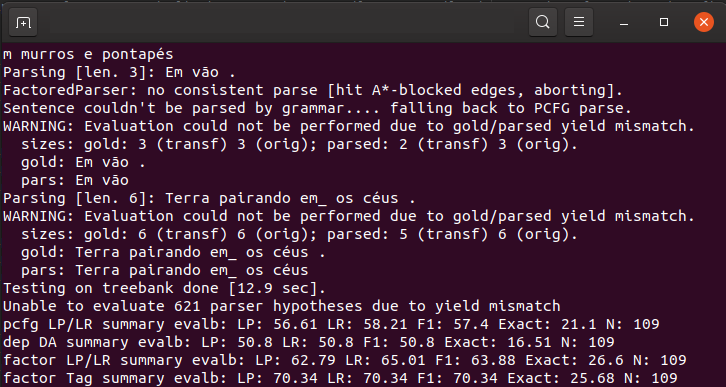
\includegraphics[width=100mm,scale=1.5]{imagens/cintil_training_error.png}
    \caption[Erro decorrente do mal posicionamento de pontuações na árvore do CINTIL]{Captura de tela de erro decorrente do mal posicionamento de pontuações na árvore do CINTIL, com relação ao formato PTB}
    \label{fig:cintil_training_error}
\end{figure}
% \end{center}

% % ------------------------------------------------------------------------------------------------
% \subsection{Treinamento}\label{treino_cintil}
% Para fazer estas conversões, fizemos um script disponível online\footnote{\url{ https://github.com/Fernandomn/separador-cintil}}.

% Com as tags convertidas, foi feito o treinamento. O ato do treino é relativamente simples: deve-se, através do terminal do seu sistema, navegar até o diretório onde se encontra o stanford-parser.jar, o arquivo que contém os parsers do SP que utilizaremos. Estando no diretório correto, deve-se executar o comando abaixo:

% \begin{center}
% \begin{lstlisting}[breaklines, caption={Execução de treinos do Stanford Parser para o CINTIL},label={lst:treinoBasicoCintil},language=Bash]
    java -cp ~/<diretorio de trabalho>/stanford-parser.jar -mx4g edu.stanford.nlp.parser.lexparser.LexicalizedParser -train ~/<diretorio do treebank>/tree-trad 1-1014 -saveToSerializedFile ~/<diretorio de armazenamento>/serialGrammarCINTIL -saveToTextFile ~/<diretorio de armazenamento>/textGrammarCINTIL
\end{lstlisting}
% \end{center}

% O código acima merece algumas explicações a parte, para quem não está familiarizado ao uso do SP pelo terminal

% \begin{center}
% \begin{table}[h!]
    \centering
    \begin{tabular}{p{0.8\textwidth}}
        \begin{itemize}
            \item [-cp] \textit{ClassPath}. Indica o diretório onde se encontra a classe principal a ser executada
            \item [-mx4g] Quantidade de memória usada. No caso, 4 GB.
            \item [LexicalizedParser] \textit{Parser} utilizado, dentre os disponibilizados
            \item [-train] Treino. Logo em seguida, um diretório e a lista de arquivos a serem usados para treinar
            \item [-saveToSerializedFile] Salva o resultado do treino num arquivo binário, cujo diretório está indicado na sequência
            \item [-saveToTextFile] Salva o resultado do treino num arquivo de texto, cujo diretório está indicado na sequência
        \end{itemize}
    \end{tabular}
    \caption[Comandos para um treino simples do \textit{Stanford Parser}]{Comandos para um treino simples do \textit{Stanford Parser}, utilizando o terminal.}
    \label{tab:tab_treino_basico_cintil}
\end{table}
% \end{center}

% A tabela \ref{tab:tab_treino_basico_cintil} mostra um fragmento das possibilidades de comandos a serem usados pela interface do terminal do SP. Note que usamos apenas 1014 arquivos nesta demonstração, que é um fração de 10\% dos arquivos / árvores do CINTIL disponíveis.

% Para melhor verificação dos resultados, utilizamos o método de \textit{10-fold cross-validation}. Este método, como explicado por \citeonline{james2013introduction},
% \begin{displayquote}
% This approach involves randomly dividing the set of observations into k groups, or folds, of approximately equal size. The first fold is treated as a validation set, and the method is fit on the remaining k -- 1 folds\footnote{\textquote{Esta abordagem envolve dividir aleatoriamente o conjunto de observações em k grupos, ou dobras, de tamanhos aproximadamente iguais. O primeiro grupo é tratado como conjunto de validação, e o método se encaixa nos k -- 1 grupos restantes}. Tradução própria.}.
% \end{displayquote}

% No nosso caso, dividimos nosso corpora em 10 partes de 1014 sentenças. Fizemos o treinamento com 1 parte, e o teste com a parte restante, alternando as partes escolhidas.  Os resultados serão apresentados na conclusão.

% Na sequencia, foi executado o treinamento com as partes restantes. De maneira análoga, no mesmo diretório, foi utilizado o seguinte comando:

% \begin{center}
% \begin{lstlisting}[breaklines, caption={Execução de testes do Stanford Parser para o CINTIL},label={lst:testeBasicoCintil},language=Bash]
    java -cp stanford-parser.jar -mx4g edu.stanford.nlp.parser.lexparser.LexicalizedParser -loadFromSerializedFile /home/fernando/projeto-final-parsers/serialized-files/serialGrammarCINTIL1 input/sentencas_teste_cintil.txt

\end{lstlisting}
% \end{center}
% Que também merece explicações, na tabela \ref{tab:tab_teste_basico_cintil}:
% \begin{center}
% \begin{table}[h!]
    \centering
    \begin{tabular}{p{0.8\textwidth}}
        \begin{itemize}
            \item [-cp] \textit{ClassPath}. Indica o diretório onde se encontra a classe principal a ser executada
            \item [-mx4g] Quantidade de memória usada. No caso, 4 GB.
            \item [LexicalizedParser] \textit{Parser} utilizado, dentre os disponibilizados
            \item [-writeOutputFiles ] Indica que os testes imprimirão arquivos de saída, a serem definidos
            \item [-outputFilesDirectory] Define o diretório onde os arquivos de saída serão escritos. 
            \item [-loadFromSerializedFile] Carrega a gramática serializada, gerada na execução de treinamento anterior
            \item [-testTreebank] Diretório onde se encontra o treebank a ser usado para teste. Os números no formato $a-b$ indicam o primeiro e o último arquivo, respectivamente. Números no formato $a-b,c-d$ indicam dois blocos de arquivos. Atente para não usar o mesmo bloco dos treinos, ou o parser passará por \textit{overfitting}, e terá resultados enviesados.
        \end{itemize}
    \end{tabular}
    \caption[Comandos para um teste simples do Stanford Parser]{Comandos para um teste simples do Stanford Parser, utilizando o terminal.}
    \label{tab:tab_teste_basico_cintil}
\end{table}
% \end{center}
% O resultado total dos testes resultou na extensa tabela \ref{tab:cintil_result_full}, que pode ser vista nos apêndices. E os comentários dos resultados pode ser encontrado em \ref{resultados_cintil}.
% ------------------------------------------------------------------------------------------------
% \section{Treinando o Stanford Parser sobre Bosque}
% \label{treinando_sp_bosque}

% Como já vimos, o Bosque é disponibilizado em duas variantes, português brasileiro (BR) e português europeu (PT). este trabalho foi feito considerando ambas, porém focando na variante brasileira. 

% Assim como o CINTIL, parte importante do nosso trabalho foi traduzir as tags do BOSQUE para o padrão PTB. Isso implicou em decisões que serão apresentadas na tabela a seguir:

% \begin{center}
%     \begin{longtable}{|p{0.1\linewidth}|p{0.2\linewidth}|p{0.15\linewidth}|p{0.15\linewidth}|p{0.3\linewidth}|}
\caption{Tabela de conversão: BOSQUE para PTB}\\
\hline
\textbf{Tag Original (Português)} & \textbf{Nome da Tag} & \textbf{Tag Convertida} & \textbf{Ocorrências} & \textbf{Observações}\\
\hline
\endfirsthead
\multicolumn{5}{c}%
{\tablename\ \thetable\ -- \textit{Continuação da página anterior}} \\
\hline
\textbf{Tag Original (Português)} & \textbf{Nome da Tag} & \textbf{Tag Convertida} & \textbf{Ocorrências} & \textbf{Observações} \\
\hline
\endhead
\hline \multicolumn{5}{r}{\textit{Continua na próxima página}} \\
\endfoot
\hline
\endlastfoot
    acl & Forma Oracional averbais & ?? & 277 & Não possui conversão direta. Melhor explicado em \ref{subsec:tag_acl}\\
    adj & adjectivos & JJ & 3484 & \\
    adjp & Sintagma adjectivais & ADJP & 3367 & \\
    adv & advérbios & RB & 3052 & \\
    advp & Sintagma adverbiais & ADVP & 2288 & \\
    art & artigos & DT & 10742 & \\
    conj-c & conjunções coordenativa & CC & 1723 & Explicado na sessão \ref{subsec:cu}\\
    conj-s & conjunções subordinativa & IN & 798 & \\
    cu & sintagma evidenciador de relação de coordenação & \_CU\_ & 1744 & Será explicado na sessão \ref{subsec:cu}\\
    ec & prefixos & \_EC\_ & 80 & Será explicado na sessão \ref{subsec:sec_ec}\\
    fcl & Forma Oracional Finita & VP & 6040 & Sentenças onde os verbos não estão no infinitivo. Sintagma verbal\\
    icl & Forma Oracional não finita & VP & 1827 & Sentenças onde os veros estão conjugados. Sintagma Verbal\\
    intj & interjeições & UH & 22 & \\
    n & substantivos & NN & 15724 & \\
    n-adj & substantivos / adjectivos & NN & 174 & Pesquisa mostrou que são todas as ocorrências são substantivos\\
    np & Sintagma nominais & NP & 22981 & \\
    num & numeral & CD & 1625 & \\
    pp & Sintagma preposicionais & PP & 11576 & \\
    pron-det & pronomes determinativos & DT & 1580 & Pelo \citeonline{posPTBguidelines}, \textquote{\textit{This category includes [\ldots] the indefinite determiners \textit{another}, \textit{any}, \textit{some}, \textit{each}, \textit{either} [\ldots], \textit{neither} [\ldots], \textit{that}, \textit{these}, \textit{this} and \textit{those} [\ldots]}}. No português, também, por \citeonline[p88]{mioto2013novo} \textquote{[\ldots] DP pode ter seu núcleo D preenchido por um item que tenha valor de determinante como artigos, demonstrativos e interrogativos[\ldots]}\\
    pron-indp & pronomes independentes & PRP & 1001 & PTB considera 4 tipos de pronomes: os pessoais, possessivos, wh-possessivos e wh-pessoais. Decidimos manter a marcação de pronomes pessoais. Isso é reforçado pela própria descrição de \citeonline{freitas2007biblia}, \textquote{pronome independente (com comportamento semelhante ao nome)}\\
    pron-pers & pronomes pessoais  & PRP & 891 & \\
    prop & nomes próprios & NNP & 4575 & \\
    prp & preposições & IN & 11694 & \\
    sq & Sintagma sequências discursivas & S & 56 & Marcador de Sentença\\
    v-fin & verbos finitos & VBP & 6167 & Verbos conjugados\\
    v-ger & verbos gerúndios & VBG & 328 & \\
    v-inf & verbos infinitivos & VB & 1684 & \\
    v-pcp & verbos particípios & VBN & 1577 & \\
    vp & Sintagma verbais & VP & 8103 & \\
    x & <desconhecido> & VB & 552 & Explicado na sessão \ref{subsec:sec_x}

\label{tab:tab_bosque}

\end{longtable}
% \end{center}

% Primeiramente, traduzimos todas as tags em sequência, mantendo a estrutura das árvores originais. Notamos, então, que para além da tradução de tags, algumas particularidades entre treebanks precisou de uma análise distinta, para maior corretude. Tais procedimentos foram executados imediatamente após, e na ordem aqui relatada.
% % ------------------------------------------------------------------------------------------------
% \subsection{Problemas com EC (Prefixos)}
% \label{sec_ec}

% Palavras marcadas com "ec", tag de prefixos, são (como o nome indica) prefixos. No caso em específico, o prefixo (ou morfema prefixal) que recebem tais marcações são aqueles ligados à palavra por hífens, como na figura \ref{fig:bosque_2166}:

% \begin{center}
%     \begin{figure}[!ht]
    % \centering
    % \includegraphics{}
    \begin{center}
        \begin{minipage}{10cm}
            \begin{tabbing}
                \=\ldots\=\+\\
                \>(>N:ec:ex-:: ex-)\\
                \>(H:n:jogador:M\_P::: jogadores)\-\\
                \>\ldots
            \end{tabbing}
        \end{minipage}
    \end{center}
    \caption[Demonstração do uso de \textquote{ec} no Bosque]{Trecho da sentença CF515-1, do Bosque: \textquote{Ex-jogadores elogiam os colunistas Telé e Cruyff}. Demonstração da aplicação da \textit{tag} \textquote{ec}.}
    \label{fig:bosque_2166}
\end{figure}
% \end{center}

% O PTB não prevê situações como estas. Pelo contrário, como podemos ver no guia de marcações do PTB \citeonline{bracketing_ptb}, tal sinal é ignorado. Recolhendo um exemplo do próprio corpus, analisemos a imagem \ref{fig:ptb_0012}

% \begin{center}
%     \begin{figure}[!h]
    % \includegraphics{}
    % wsj\_0012: In mid-October, Time magazine lowered its guaranteed [\ldots]\\\\
    \centering
    \begin{minipage}{10cm}
        \ldots
        \begin{tabbing}
        \centering
            \=( (S (S \=\+\\
            \>(PP-TMP In\=\+\\
            \>(NP \textbf{mid-October})\-\\
            \>),\\
            \>(NP-SBJ-1 Time magazine)\\
            \>(VP lowered\\
        \end{tabbing}
        \ldots
    \end{minipage}
    
    \caption[Fragmento da sentença wsj\_0012, do PTB, sobre aplicação de prefixos]{Fragmento da sentença wsj\_0012, do PTB: \textquote{\textit{In mid-October, Time magazine lowered its guaranteed circulation rate base for 1990 while not increasing ad page rates; with a lower circulation base, Time's ad rate will be effectively 7.5\% higher per subscriber; a full page in Time costs about \$120,000.}}}
    \label{fig:ptb_0012}
\end{figure}
% \end{center}

% A flexão \textquote{mid-October} é representada, sozinha, como um sintagma nominal (\textit{noun phrase}). Portanto, fez-se necessário a criação de uma subtarefa que removesse tais tags, e que a estrutura fosse refeita, de modo a seguir os padrões do PTB. 

% % ------------------------------------------------------------------------------------------------
% \subsection{Problemas com CU (Coordenação)}
% \label{sec_cu}
% Coordenação é talvez a tag mais problemática do BOSQUE. Como destacam \citeonline{Wing2006Adaptation}, 
% \begin{quote}
%     Conjoined clauses in the native Floresta are of type CU, regardless of the type of constituents being conjoined. This causes grammars learned from the treebank to make errors such as conflating noun phrase conjunctions and sentential conjunctions.
%     \footnote{\textquote{Cláusulas conjuntivas no Floresta nativo são do tipo CU, independentemente do tipo de constituinte conjunto. Isso faz com que a gramática aprendida do treebank cometa erros como confundir conjunções de sintagmas nominais e conjunções sentenciais}. Tradução própria.}.
% \end{quote}
% O PTB tem suas próprias regras para determinar a estrutura de coordenações, reservando o capítulo 7 de seu Manual de Agrupamento (\citeonline{bies95pennbracketing}). Seguindo tais regras, num primeiro momento de tradução, apenas marcamos as coordenações com a tag auxiliar \_CU\_. Depois, fizemos uma nova verificação, reconhecendo as sentenças onde essa marca aparece. Ao encontrá-las, reconstruímos as árvores na estrutura de listas encadeadas, para que pudéssemos fazer a análise dos filhos deste nó (CU) de maneira precisa.  A partir dele, seguimos a regra do Bracketing Guide, para traduzir a tag corretamente. Tal script está disponível para verificação\footnote{\url{https://github.com/Fernandomn/separa-bosque}}. 
% % ------------------------------------------------------------------------------------------------
% \subsection{Tag X}
% \label{sec_x}
% Por todo corpora, pode ser encontrado o par de tags, X e x. X é uma tag do tipo função, e x, uma POS tag. Ela aparece, recorrentemente, próxima à coordenações, mas no guia oficial do Bosque, o Bíblia Florestal\footnote{https://www.linguateca.pt/floresta/BibliaFlorestal/}, não há uma descrição formal para a mesma. Para evitar uma possível imprecisão ao traduzí-la, decidimos por remover do corpus as sentenças que a apresentam. Tal par ocorre em 981 casos, equivalente a <...> sentenças, correspondente a <..>\% do Bosque.







% ---------------------------------------------------------------
% \section{Resultados}
\label{resultados}
Daqui em diante, mostraremos os resultados dos experimentos, separados por cada um dos \textit{corpus} base. Ao final desta seção, será feito um debate acerca dos resultados alcançados.

Os testes foram feitos utilizando um computador Intel Core i7-7700HQ de 64bits, com 16GB de memória RAM.
\subsection{Resultados do CINTIL}
\label{subsec:resultados_cintil}
Nesta sessão, demonstraremos os resultados obtidos com a transdução do CINTIL.

\subsubsection{Treinamento} 
\label{subsubsec:result_treino_cintil}

Na Tabela \ref{tab:resultados_treino_cintil}, podemos ver o relatório de treinamento de cada execução do SP com o CINTIL transduzido.
\begin{center}
    \input{tabelas/tab_cintil_result_treino.tex}
\end{center}

% Pode-se notar que bons resultados de treino são obtidos apenas com o primeiro \textit{fold}, cujos resultados superam os outros \textit{folds}. 
Pode-se notar que, além do primeiro \textit{fold} (que abrange os últimos nove décimos do \textit{treeebank} para treinamento, e reserva o primeiro para testes), os resultados são bastante semelhantes. Deduz-se, então, que o primeiro décimo do \textit{dataset} é muito relevante no processo de treino. O sexto \textit{fold} (reserva a 6ª parte para testes) parece ser o com melhores resultados gerais. 
Melhor visualizado na Figura \ref{fig:treino_cintil}.
\begin{center}
    \input{imagens/cintil_treino_result.tex}
\end{center}

As colunas necessitam de explicações, cuja coleta foi trabalhosa. O FAQ do SP é pouco informativo, e o do CoreNLP possui a mesma dificuldade.

Pelo código-fonte do SP\footnote{A referência foi a classe LexicalizedParser.java, que está disponível em \url{https://github.com/chbrown/stanford-parser/blob/master/edu/stanford/nlp/parser/lexparser/LexicalizedParser.java}}, \textit{States} representa a quantidade de Índices de Estado. Inferiu-se que é a quantidade de estados de transição da gramática gerada pelo treino. 

\textit{Tags}, por sua vez, representa a quantidade de Índices de \textit{Tags}. Seria a quantidade de \textit{Tags} registradas durante o treino (note que o número varia pouco).

\textit{Words}, de forma análoga, representa a quantidade de Índices de Palavras. Deduz-se que, a quantidade de palavras distintas verificadas pelo treinamento.

\textit{UnaryR} e \textit{BinaryR} correspondem, respectivamente, às quantidades de regras das gramáticas Unária e Binária. A descrição de ambas classes é, na sequencia, \textquote{\textit{Maintains efficient indexing of unary grammar rules}} e \textquote{\textit{Maintains efficient indexing of binary grammar rules}}. Pelo Javadoc do SP\footnote{\url{https://nlp.stanford.edu/nlp/javadoc/javanlp/edu/stanford/nlp/parser/lexparser/package-summary.html}},
\begin{quote}
    \begin{itemize}
        \item \textit{Unary Grammar - consists of unary rewrite rules, one per line, each of which is of the form A -> B, followed by the normalized log probability.}
        \footnote{Gramática Unária - consiste em regras de reescrita unárias, uma por linha, cada qual na forma A -> B, seguida pela probabilidade log normalizada}
        \item \textit{Binary Grammar - consists of binary rewrite rules, one per line, each of which is of the form A -> B C, followed by the normalized log probability.}
        \footnote{Gramática Binária - consiste em regras de reescrita binárias, uma por linha, cada qual na forma A -> B C, seguida pela probabilidade log normalizada}
    \end{itemize}
\end{quote}

Cabe frisar que tal modelo, utilizando regras unárias e binárias, segue o padrão da Forma Normal de Chomsky, que pode ser visto em \cite[p~389]{Manning1999FoundationsNLP}.

Por fim, \textit{Taggings} se refere à \textquote{\textit{[\ldots]the number of rules (tag rewrites as word) in the Lexicon.}}
\footnote{o número de regras (etiquetas reescritas como palavras) no Lexicon}.
Lexicon é uma interface, descrita como
\begin{quote}
    \textquote{\textit{An interface for lexicons interfacing to lexparser. Its primary responsibility is to provide a conditional probability P(word|tag), which is fulfilled by the {\#score} method. Inside the lexparser, Strings are interned and tags and words are usually represented as integers.}}
    \footnote{\textquote{Uma interface entre lexicons e o lexparser. Sua responsabilidade primária é prover uma probabilidade condicional P(palavra|etiqueta), que é preenchida pelo método \textit{\#score}. Dentro do \textit{lexparser}, \textit{Strings} são representadas canonicamente, e etiquetas e palavras são geralmente representadas por inteiros}. Tradução própria.}
\end{quote}

\subsubsection{Avaliação} 
\label{subsubsec:result_aval_cintil}

Nos apêndices, a Tabela \ref{tab:cintil_result_full} traz os resultados completos de nossos testes com o CINTIL. Vamos usar, aqui, versões reduzidas dos dados.

Começando pelos dados da PCFG interna ao LexicalizedParser, podemos ver o seu resultado na Tabela \ref{tab:result_cintil_pcfg}, e na Figura \ref{fig:cintil_result_pcfg}.
\begin{center}
    \input{tabelas/tab_resultados_cintil_pcfg.tex}
\end{center}

A média da \textit{F1-Score} é 59.304\%, e seu desvio padrão é de aprox. 4.208\%.

Fica claro que a simples transdução de árvores da língua portuguesa para os padrões da língua inglesa, conservando as palavras, é insuficiente para o bom resultado do \textit{parser}.

% Nota-se, também, que para classificações mais eficientes, bastaria utilizar o primeiro décimo do CINTIL, pois tal bloco superou todos os outros durante o treino.
\begin{center}
    \input{imagens/cintil_result_pcfg.tex}
\end{center}

\subsubsection{Estudos de caso}
\label{subsubsec:ec_cintil}

Separamos alguns exemplos de sentenças transduzidas, classificadas pelo \textit{Stanford Parser}. Serão exibidas as sentenças já em formato de árvore. As imagens foram produzidas no \textit{website} jsSyntaxTree\footnote{\url{http://www.ironcreek.net/syntaxtree/}}.

O \textit{parsing} do PS é feito executando o comando \ref{lst:cod_parsing_cintil}. Note que utilizamos a gramática treinada pelo sexto \textit{fold}.
\begin{center}
    \input{codigos/cod_parsing_cintil.tex}
\end{center}

Explicando rapidamente na Tabela \ref{tab:tab_exec_basico_cintil}.

\begin{center}
    \input{tabelas/tab_CintilExecBasica.tex}
\end{center}

\begin{center}
    \input{imagens/ec_cintil_sem_ponto_tree.tex}
\end{center}

Na Figura \ref{fig:ec_cintil_sem_ponto_tree}, vemos o resultado da classificação de uma sentença originalmente sem pontuações. Há algumas coisas interessantes a serem notadas. Se, por um lado, de fato a falta de pontuação ajudou no \textit{parsing}, 
% por outro o SP tem dificuldades em separar contrações de preposições.
as contrações de preposição (\textquote{à}, \textquote{no}) não são identificados. O que faz sentido, pois o treino foi feito considerando tais separações.

\begin{center}
    \input{imagens/ec_cintil_conjp_tree.tex}
\end{center}

A Figura \ref{fig:ec_cintil_conjp_tree} nos dá mais material de interesse. 
% Por exemplo, pode-se notar como a ausência de conhecimento de léxico da língua classificada gera confusões. 
% O \textquote{o} é facilmente confundido, mas não apenas. 
% O sintagma CONJP, que some na árvore transduzida, retorna na árvore classificada. Interessante notar que a 
% que a transforma num adjunto de VP. 
% O sintagma VP, em \textquote{não podia} tem seu núcleo, e por conseguinte, o sintagma como um todo, alterado. Provavelmente, para seguir a tendência da língua inglesa, que costuma ter o núcleo do sintagma posicionado mais à direita \cite[p~40]{charniak97statistical}. 
% A confusão com as pontuações é notável, sendo transformadas em substantivo (NNS) ou verbo (VB), o que é curioso. 
% Supões-se que o SP não seja estranho à pontuações mesmo que elas não venham no seu conjunto de treino.
A confusão gerada pela falta de treinamento sobre pontuações permanece, sendo ainda uma das maiores falhas. O $VP_3$ \textquote{não aconteça} se torna um $ADJP$, considerando como núcleo o advérbio \textquote{não}. O esforço de manter a estrutura de conjunções, que estudamos na Seção \ref{subsec-cintil-conj} é desfeito, convertendo o sintagma solto em \textit{flat structure} \textquote{para que} se converte num PP. Vale notar que ele não se torna um sintagma conjuntivo (CONJP), e \textquote{que} não é marcado como CC, que é a tendência tradicional do \textit{parser}. Também, apesar da tendência da língua inglesa, que costuma ter o núcleo do sintagma posicionado mais à direita \cite[p~40]{charniak97statistical}, isso não ocorre nem no PP, nem no ADJP.

\begin{center}
    \input{imagens/ec_cintil_cp_tree.tex}
\end{center}

Verificando as alterações realizadas sobre o sintagma CP, como vimos na Seção \ref{subsec-cintil-c}, vejamos a Figura \ref{fig:ec_cintil_cp_tree}. Curiosamente, o sintagma em questão está acompanhando bem a estrutura da árvore original, e da árvore transduzida. 
% O maior destaque ficam para as palavras de classe aberta (substantivos, verbos, adjetivos). Aparentemente, a informação léxica continua sendo um problema.
\begin{center}
    \input{imagens/ec_cintil_virgula_tree.tex}
\end{center}

Para finalizar nossa revisão com as transduções do CINTIL, temos a Figura \ref{fig:ec_cintil_virgula_tree}, a respeito da colocação de vírgulas.
Pode-se notar a dificuldade léxica, onde palavras como \textquote{vistos} e \textquote{adiadas} são confundidos. Acredita-se que, se a contração da palavra \textquote{pelos} fosse detectada, a presença do Determinante resolveria tal problema. Os erros de marcação destes terminais afetam toda a marcação da árvore acima. Curioso notar também que, sem o treino de pontuações, tais símbolos se tornam ou substantivos (NNS), ou adjetivos (JJ). Porém, nem sempre são marcadas da mesma maneira, como pode ser comparado entre as Figuras \ref{fig:ec_cintil_virgula_tree} e \ref{fig:ec_cintil_conjp_tree}.
% Nota-se uma tendência muito interessante, do SP, de considerar palavras como adjetivo (JJ). Mesmo para palavras que nunca assumem tal forma, como \textquote{pelos}, que pode ser ou a contração \textit{por + os}, ou um substantivo. A falta de treinamento com pontuações mais uma vez é sentida, uma vez que SP não sabe como resolver vírgulas e pontos.
\subsection{Resultados do Bosque}
\label{subsec:resultados_bosque}
Neste momento, serão mostrados os resultados das execuções baseadas no BOSQUE.

\subsubsection{Treinamento} 
\label{subsubsec:result_treino_bosque}
Na Tabela \ref{tab:resultados_treino_bosque}, vemos os resultados dos treinamentos do SP sobre Bosque transduzido por nós. Note que os campos são equivalentes aos explicados em \ref{result_treino_cintil}.
\begin{center}
    \input{tabelas/tab_bosque_result_treino.tex}
\end{center}

A Figura \ref{fig:treino_bosque} nos dá a visualização desses resultados. Pode-se observar que o resultado pre-eliminar dos testes é muito superior ao visualizado em \ref{result_treino_cintil}.
\begin{center}
    \input{imagens/bosque_treino.tex}
\end{center}

\subsubsection{Avaliação} 
\label{subsubsec:result_aval_bosque}
Na Tabela \ref{tab:result_bosque_pcfg}, vemos o resultados dos testes utilizando o SP sobre o Bosque transduzido.
\begin{center}
    \input{tabelas/tab_bosque_result_pcfg.tex}
\end{center}

A média da \textit{F1-Score} é de 49.551\%, e tem o desvio padrão de aprox. 1.992\%.

Na Figura \ref{fig:bosque_result_pcfg} podemos ter uma visualização melhor de tais resultados.
\begin{center}
    \input{imagens/bosque_result_pcfg.tex}
\end{center}

É possível notar que, mesmo com o desempenho de treinamento melhor que os do CINTIL (como visto em \ref{result_treino_cintil}), a classificação continua tendo uma qualidade baixa. 
% nunca superando os 50\%.
Apenas os dois últimos \textit{folds} superam os 50\%.

\subsubsection{Estudos de caso}
\label{subsec:ec-bosque}

De modo análogo ao do CINTIL, vamos revisar aqui alguns casos curiosos de sentenças classificadas. Utilizaremos a gramática do décimo treino para as classificações e avaliações. O Bosque tem mais casos problemáticos que o CINTIL, e visualizar todas elas tornaria este trabalho ainda maior. Portanto, alguns casos serão exibidos apenas nos Apêndices.
\begin{center}
    \input{imagens/ec_bosque_sem_ponto_tree.tex}
\end{center}

A Figura \ref{fig:ec_bosque_sem_ponto_tree} nos mostra as diferenças entre árvores sem pontuação. Foram removidas as informações adicionais dos nós da árvore original do Bosque, mantendo apenas $(F:f)$.
Temos poucos erros de \textit{parsing}. Nenhum nó terminal foi classificado erroneamente, apenas nós internos (não-terminais). Uma ambiguidade no $NP$ de \textquote{12 páginas}, que agora abarca também o $PP$ irmão. 
% E o núcleo do primeiro $NP$, que foi classificado como $NP$.

\begin{center}
    \input{imagens/ec_bosque_komp_tree.tex}
\end{center}

A Figura \ref{fig:ec_bosque_komp_tree} traz uma sentença que, originalmente, possui o par $KOMP<:acl$ internamente. É notório como as regras unárias (Não-terminal $\rightarrow$ terminal) são mais consistentes que as binárias. Curioso também a separação de palavras originalmente conjuntas, como \textquote{por exemplo} e \textquote{do que}. Ambas expressões aparecem pouco no CETEMFolha (22 e 34 vezes, respectivamente). Porém, pelas observações anteriores, supõe-se que o SP não está pronto para lidar com nós terminais concatenados durante a execução. 
% Cabe observar que a estrutura de Comparação foi mantida no estilo PTB, como visto em \ref{fig:ec_bosque_komp_detalhe}, apesar da discordância entre $SBAR$ (transdução) e $PP$ (\textit{Stanford}).
Interessante notar que a estrutura de Comparação (estudada em \ref{subsec:tag_komp}) foi desfeita pelo SP.

\begin{center}
    \input{imagens/ec_bosque_ec_tree.tex}
\end{center}

A Figura \ref{fig:ec_bosque_ec_tree}
% vem com uma novidade inusitada: Foi considerada agramatical pelo \textit{parser} fatorado, disponibilizado pelo SP (que não abordamos neste trabalho). Mas foi interpretado pelo PCFG. 
traz um fato inesperado: a ideia com esta sentença era estudar a aplicação da \textit{tag} \textit{ec}, que inclusive não apresentou problemas. Mas a conjunção \textquote{parentes e amigos} foi desfeita pelo SP. \textquote{E} se tornou um mero irmão dos dois sintagmas, tal qual uma vírgula, e recebeu a \textit{tag} $CC$, que pouco aparece devido às conversões feitas na transdução para que o $SP$ aceitasse conjunções. O mesmo ocorre no \textit{parsing} da sentença CF318-C (fragmento em \ref{fig:ec_bosque_komp_detalhe}), mostrando que, apesar deste trabalho ter se guiado pelo \textit{Bracketing Guidelines} \cite{bracketing_ptb}, algumas estruturas poderiam se manter equivalentes às apresentadas no Bosque.

Outras análises serão apresentadas nos apêndices.
\subsection{Comentários}
\label{subsec:result_coment}

Fica claro, pela observação dos dados abordados, que a transdução de \textit{datasets} pode não ser o melhor caminho para suprir a necessidade de \textit{parsers} para o Português. Porém, existem algumas considerações que precisam ser feitas.

Primeiramente, deve-se notar como é curioso que, apesar do treino do SP com dados transduzidos pelo CINTIL possuírem uma maior quantidade de dados, os resultados do treino deste (visto na Tabela \ref{tab:resultados_treino_cintil}) são bastante tímidos, se comparados com os números da mesma operação sobre o Bosque (Tabela \ref{tab:resultados_treino_bosque}). Podemos levantar algumas hipóteses: 
\begin{itemize}
    \item A maior quantidade de dados permitiu que o SP tivesse mais acesso à árvores problemáticas, fazendo com que o resultado geral fosse inferior;
    \item Apesar do tamanho do Bosque ser menor, suas árvores são mais completas, permitindo maior generalização;
    \item A transdução dos dados do Bosque foi feita de forma mais acurada, permitindo um treinamento melhor.
\end{itemize}
É curioso notar, por exemplo, como o SP registrou mais \textit{tags} sobre o Bosque do que sobre o CINTIL. Observar as Tabelas \ref{tab:tab_cintil} e \ref{tab:tab_bosque} poderia ser uma alternativa, mas não se justifica: Foram usadas 20 \textit{tags} na transdução do Bosque, contra\ldots 20 do CINTIL. Mesmo com as duas tabelas de possibilidades do Bosque, para alguns casos (como comentado em \ref{subsec:sec_x} \ref{subsec:tag_acl}). A quantidade de regras gramaticais apreendidas quando nos baseamos no Bosque, também, é de um contraste muito interessante: no melhor caso do treinamento sobre CINTIL (\textit{fold 1}), foram aprendidas 257 regras, contra 1027 do pior caso do treino com o Bosque (\textit{fold 10}). Observar as Figuras \ref{fig:treino_cintil} e \ref{fig:treino_bosque} nos permite ver essas diferenças.

Uma olhada mais atenta às \textit{tags} utilizadas pode nos dar uma pista. Como pode-se ver na Tabela \ref{tab:comp_cintil_bosque}, basicamente foram usadas as mesmas \textit{tags}. As diferenças expressivas estão, no CINTIL, no uso repetitivo das interjeições, e no uso de CONJP. Bosque, por outro lado, tem uma pluralidade maior de marcações relativas à verbos. Retornar à Tabela \ref{tab:tab_bosque} nos faz ver que tal característica vem desde o \textit{treebank} original. 
\begin{center}
    \input{tabelas/tab_comp_tags_bosque_cintil.tex}
\end{center}

Seria o caso, então, de uma maior atenção no desenvolvimento da solução para um \textit{dataset} do que para o outro? Pode-se afirmar que não. Toda alteração feita, como já dito ao longo do trabalho, foi com o objetivo de fazer com que o \textit{Stanford Parser} fosse capaz de receber as florestas sintáticas transduzidas. Toda alteração e desenvolvimento foram feitos pensando no mínimo necessário para que o processamento fosse possível. Com isso, quer-se dizer que: A ambos conjuntos de dados, foi dada atenção equivalente.
% pois o objetivo deste trabalho não era fazer uma adaptação perfeita. 
Código foi escrito na medida que o SP, e os \textit{treebanks} \textquote{exigiam}.
% Para citar um fato, em \ref{subsec:percent} comentamos que precisamos excluir as sentenças que incluíam \textquote{\%} em seu corpo. Isso dá um total de 149 sentenças, aprox. 3,5\% do \textit{dataset} completo.
\begin{center}
    \input{imagens/comp_F1_cintil_bosque.tex}
\end{center}
O que nos leva a um novo problema: ambos \textit{datasets} tiveram resultados baixos de \textit{F1-score}, variando entre 41\% e 45\%. A Figura \ref{fig:comp_f1_cintil_bosque} permite melhor visualização.
% Tal fato também nos faz levantar algumas hipóteses.
As seções \ref{result_aval_cintil} e \ref{result_aval_bosque} nos fazem entender o motivo. O mesmo conjunto de dados foi usado tanto para o treino como para os testes. Porém, ao executar sentenças reais, os resultados são sofríveis. Deve-se levar em consideração os pontos abordados sobre as características da métrica de avaliação em \ref{subsec:parseval}, é claro. Mas é inegável: os \textit{parse} obtidos estão muito aquém do esperado. 

A observação mais próxima desses resultados indica uma possível resposta: o \textit{Stanford Parser} está muito atrelado às regras lexicais do Inglês. O que faz todo sentido, quando lembramos que deliberadamente optamos por usar tal \textit{parser}. Mais: ao optar-se por não fazer grandes desenvolvimentos a partir dele, ou até mesmo não utilizar modelos de outras linguagens que estão disponíveis e distribuídos oficialmente, era sabido que o modelo padrão que compõe o SP é o da língua inglesa. Portanto, em nada otimizado para o português, qualquer variante que seja. 

Faz todo o sentido retomar este trabalho no futuro, aprimorar suas características, e torná-lo mais preciso, sem que seja necessário descartar nenhuma sentença que seja. A ausência de pontuações é muito sentida no \textit{score} final. Mas, estamos convencidos: Transdutores não são a solução para o problema da ausência de \textit{parsers} para o Português.

Ou melhor, não sozinhos. Transduzir os dois \textit{datasets}, de modo que o SP fosse capaz de processá-las foi um grande avanço. Isto torna uma potencial nova etapa possível, essa sim podendo ser a resposta: adaptar o SP para o Português. Produzir um novo modelo de linguagem para a ferramenta parece ser uma alternativa plausível.

Esta ideia não é nova, o LX-Parser (\citeonline{Branco2010OutOfTheBox} e \citeonline{silva-etal-2010-top}) foi desenvolvido justamente com este pensamento. Mas se encontra obsoleto. Além de que, foi necessário usar um novo \textit{dataset} no seu desenvolvimento. Criar transdutores que adaptem florestas sintáticas pré-existentes pode ser um avanço nesta parte do desenvolvimento. Isto, claro, se pensarmos num desenvolvimento já apoiado em ferramentas e bibliotecas pré-existentes. Desenvolver um \textit{parser} novo sempre é uma possibilidade.

Por fim, precisamos voltar à pergunta levantada em \ref{cha:introducao} e \ref{sec:contexto}: seria possível a alguém, com pouco conhecimento acadêmico, realizar tarefa semelhante ao do trabalho apresentado? A resposta é: Dificilmente. 

Desenvolver os transdutores exigiu uma certa gama de conhecimentos interessantes e multidisciplinares. Fora algumas necessidades. Ter um computador, por exemplo. Suponhamos que ela tenha um computador, e não seja estranha à equipamentos eletrônicos. Ela vai precisar aprender a programar. A linguagem de programação deste trabalho foi Python, que tem baixa dificuldade de aprendizado inicial. Ótimo começo. A pessoa em questão precisa saber o básico de manipulação de \textit{strings}, o que por sorte, costuma ser um dos aprendizados iniciais. As facilidades param por aí. Construir o transdutor exige o conhecimento de estruturas de dados, para que a estrutura simbólica das árvores seja reproduzida logicamente. Por conseguinte, é preciso também ser capaz de manipular tais árvores. Pode-se ter uma noção intuitiva disto, mas não é um assunto trivial. Também, exige que ela tenha conhecimento de árvores de constituência. Dependendo do histórico de vida desta pessoa, ela viu algo semelhante na escola. Mas é um conhecimento de cursos de licenciatura / bacharelado em letras. Também, o transdutor exige multidisciplinaridade do desenvolvedor. É preciso ter disposição para programar, assim como de ler gramáticas para estudar regras gramaticais e linguísticas. Não ter esses conhecimentos implicará em código ruim. 

Mais: me referi apenas à construção dos transdutores. Para a construção de \textit{parsers}, será necessário um bom conhecimento de estatística, e de desenvolvimento em inteligência artificial. Como mostramos em \ref{subsec:statisticalparsing}, nem só a estatística será suficiente para se obter um \textit{parser} utilizável.

Fica, então, a dúvida: uma pessoa que queira usar um \textit{parser} precisa mesmo de tudo isso? Bastaria usar os disponíveis. Mas, como já citado ao longo deste trabalho, existem poucos disponíveis. E \textit{parsers} podem ser úteis para o público geral. No aprendizado de línguas, nativa ou estrangeira, ou tradução, por exemplo. Se esta pessoa hipotética não conseguir achar algum \textit{parser} que lhe seja útil, ela seria capaz de construir um por conta própria?

A resposta otimista é: Esperamos que sim. Muito material de estudo está disponível gratuitamente e de forma acessível. A resposta pessimista é que sem bagagens prévias de conhecimento, será muito complicado. Boa sorte aos futuros desenvolvedores.
 % Desenvolvimento
\section{Resultados}
\label{resultados}
Daqui em diante, mostraremos os resultados dos experimentos, separados por cada um dos \textit{corpus} base. Ao final desta seção, será feito um debate acerca dos resultados alcançados.

Os testes foram feitos utilizando um computador Intel Core i7-7700HQ de 64bits, com 16GB de memória RAM.
\subsection{Resultados do CINTIL}
\label{subsec:resultados_cintil}
Nesta sessão, demonstraremos os resultados obtidos com a transdução do CINTIL.

\subsubsection{Treinamento} 
\label{subsubsec:result_treino_cintil}

Na Tabela \ref{tab:resultados_treino_cintil}, podemos ver o relatório de treinamento de cada execução do SP com o CINTIL transduzido.
\begin{center}
    \begin{table}[h!]
    \centering
    % \begin{tabular}{c|c}
    %      &  \\
    %      & 
    % \end{tabular}
    \csvautotabular{tabelas/resultados_cintil_treino.csv}
    \caption{Resultados dos treinamentos do CINTIL, para os 10 \textit{folds}}
    \label{tab:resultados_treino_cintil}
\end{table}
\end{center}

% Pode-se notar que bons resultados de treino são obtidos apenas com o primeiro \textit{fold}, cujos resultados superam os outros \textit{folds}. 
Pode-se notar que, além do primeiro \textit{fold} (que abrange os últimos nove décimos do \textit{treeebank} para treinamento, e reserva o primeiro para testes), os resultados são bastante semelhantes. Deduz-se, então, que o primeiro décimo do \textit{dataset} é muito relevante no processo de treino. O sexto \textit{fold} (reserva a 6ª parte para testes) parece ser o com melhores resultados gerais. 
Melhor visualizado na Figura \ref{fig:treino_cintil}.
\begin{center}
    \begin{figure}[!ht]
    \centering
    % \includegraphics{}
    \includesvg[width=.8\textwidth]{imagens/treino_cintil}
    % \includesvg{imagens/cintil_pcfg}
    \caption[Gráfico de resultados do treinamento, usando o CINTIL transduzido]{Gráfico de resultados do treinamento do LexicalizedParser, usando o CINTIL transduzido}
    \label{fig:treino_cintil}
\end{figure}
\end{center}

As colunas necessitam de explicações, cuja coleta foi trabalhosa. O FAQ do SP é pouco informativo, e o do CoreNLP possui a mesma dificuldade.

Pelo código-fonte do SP\footnote{A referência foi a classe LexicalizedParser.java, que está disponível em \url{https://github.com/chbrown/stanford-parser/blob/master/edu/stanford/nlp/parser/lexparser/LexicalizedParser.java}}, \textit{States} representa a quantidade de Índices de Estado. Inferiu-se que é a quantidade de estados de transição da gramática gerada pelo treino. 

\textit{Tags}, por sua vez, representa a quantidade de Índices de \textit{Tags}. Seria a quantidade de \textit{Tags} registradas durante o treino (note que o número varia pouco).

\textit{Words}, de forma análoga, representa a quantidade de Índices de Palavras. Deduz-se que, a quantidade de palavras distintas verificadas pelo treinamento.

\textit{UnaryR} e \textit{BinaryR} correspondem, respectivamente, às quantidades de regras das gramáticas Unária e Binária. A descrição de ambas classes é, na sequencia, \textquote{\textit{Maintains efficient indexing of unary grammar rules}} e \textquote{\textit{Maintains efficient indexing of binary grammar rules}}. Pelo Javadoc do SP\footnote{\url{https://nlp.stanford.edu/nlp/javadoc/javanlp/edu/stanford/nlp/parser/lexparser/package-summary.html}},
\begin{quote}
    \begin{itemize}
        \item \textit{Unary Grammar - consists of unary rewrite rules, one per line, each of which is of the form A -> B, followed by the normalized log probability.}
        \footnote{Gramática Unária - consiste em regras de reescrita unárias, uma por linha, cada qual na forma A -> B, seguida pela probabilidade log normalizada}
        \item \textit{Binary Grammar - consists of binary rewrite rules, one per line, each of which is of the form A -> B C, followed by the normalized log probability.}
        \footnote{Gramática Binária - consiste em regras de reescrita binárias, uma por linha, cada qual na forma A -> B C, seguida pela probabilidade log normalizada}
    \end{itemize}
\end{quote}

Cabe frisar que tal modelo, utilizando regras unárias e binárias, segue o padrão da Forma Normal de Chomsky, que pode ser visto em \cite[p~389]{Manning1999FoundationsNLP}.

Por fim, \textit{Taggings} se refere à \textquote{\textit{[\ldots]the number of rules (tag rewrites as word) in the Lexicon.}}
\footnote{o número de regras (etiquetas reescritas como palavras) no Lexicon}.
Lexicon é uma interface, descrita como
\begin{quote}
    \textquote{\textit{An interface for lexicons interfacing to lexparser. Its primary responsibility is to provide a conditional probability P(word|tag), which is fulfilled by the {\#score} method. Inside the lexparser, Strings are interned and tags and words are usually represented as integers.}}
    \footnote{\textquote{Uma interface entre lexicons e o lexparser. Sua responsabilidade primária é prover uma probabilidade condicional P(palavra|etiqueta), que é preenchida pelo método \textit{\#score}. Dentro do \textit{lexparser}, \textit{Strings} são representadas canonicamente, e etiquetas e palavras são geralmente representadas por inteiros}. Tradução própria.}
\end{quote}

\subsubsection{Avaliação} 
\label{subsubsec:result_aval_cintil}

Nos apêndices, a Tabela \ref{tab:cintil_result_full} traz os resultados completos de nossos testes com o CINTIL. Vamos usar, aqui, versões reduzidas dos dados.

Começando pelos dados da PCFG interna ao LexicalizedParser, podemos ver o seu resultado na Tabela \ref{tab:result_cintil_pcfg}, e na Figura \ref{fig:cintil_result_pcfg}.
\begin{center}
    \begin{table}[!h]
    \centering
    \begin{tabular}{|l|c|c|c|}
        \hline
        pcfg LP/LR & LP & LR & F1\\
        \hline
        fold 1 & 58.09 & 65.99 & 61.79\\
        fold 2 & 62.52 & 62.32 & 62.42\\
        fold 3 & 55.69 & 54.58 & 55.13\\
        fold 4 & 54.03 & 51.31 & 52.63\\
        fold 5 & 61.48 & 64.64 & 63.02\\
        fold 6 & 58.81 & 57.61 & 58.21\\
        fold 7 & 62.51 & 63.67 & 63.09\\
        fold 8 & 53.03 & 54.05 & 53.54\\
        fold 9 & 61.76 & 57.5 & 59.56\\
        fold 10 & 63.32 & 63.98 & 63.65\\
        \hline
    \end{tabular}
    % \csvautotabular{resultados-cintil-testes-pcfg.csv}
    \caption{Resultados do treinamento da PCFG do SP, usando dados do CINTIL}
    \label{tab:result_cintil_pcfg}
\end{table}
        % fold 1 & 45.43 & 45.04 & 45.24\\
        % fold 2 & 42.87 & 46.27 & 44.5\\
        % fold 3 & 39.8 & 42.86 & 41.27\\
        % fold 4 & 43.55 & 47.44 & 45.42\\
        % fold 5 & 41.82 & 43.7 & 42.74\\
        % fold 6 & 41.24 & 43.26 & 42.23\\
        % fold 7 & 44.51 & 45.43 & 44.97\\
        % fold 8 & 41.61 & 44.06 & 42.8\\
        % fold 9 & 38.85 & 44.39 & 41.43\\
        % fold 10 & 39.92 & 44.13 & 41.92\\
\end{center}

A média da \textit{F1-Score} é 59.304\%, e seu desvio padrão é de aprox. 4.208\%.

Fica claro que a simples transdução de árvores da língua portuguesa para os padrões da língua inglesa, conservando as palavras, é insuficiente para o bom resultado do \textit{parser}.

% Nota-se, também, que para classificações mais eficientes, bastaria utilizar o primeiro décimo do CINTIL, pois tal bloco superou todos os outros durante o treino.
\begin{center}
    \begin{figure}[!ht]
    \centering
    % \includegraphics{}
    \includesvg[width=.8\textwidth]{imagens/cintil_pcfg}
    % \includesvg{imagens/cintil_pcfg}
    \caption[Gráfico de resultados dos testes usando o CINTIL transduzido]{Gráfico de resultados dos testes do PCFG do LexicalizedParser, usando o CINTIL transduzido}
    \label{fig:cintil_result_pcfg}
\end{figure}
\end{center}

\subsubsection{Estudos de caso}
\label{subsubsec:ec_cintil}

Separamos alguns exemplos de sentenças transduzidas, classificadas pelo \textit{Stanford Parser}. Serão exibidas as sentenças já em formato de árvore. As imagens foram produzidas no \textit{website} jsSyntaxTree\footnote{\url{http://www.ironcreek.net/syntaxtree/}}.

O \textit{parsing} do PS é feito executando o comando \ref{lst:cod_parsing_cintil}. Note que utilizamos a gramática treinada pelo sexto \textit{fold}.
\begin{center}
    \begin{lstlisting}[breaklines, caption={Execução de \textit{parsing} em sentenças transduzidas a partir do CINTIL},label={lst:cod_parsing_cintil},language=Bash]
    java -cp stanford-parser.jar -mx4g edu.stanford.nlp.parser.lexparser.LexicalizedParser -loadFromSerializedFile ~/<diretorio de armazenamento>/serialGrammarBOSQUE1 sentencas_teste_cintil.txt
\end{lstlisting}
\end{center}

Explicando rapidamente na Tabela \ref{tab:tab_exec_basico_cintil}.

\begin{center}
    \begin{table}[h!]
    \centering
    \begin{tabular}{p{0.8\textwidth}}
        \begin{itemize}
            \item [-cp] \textit{ClassPath}. Indica o diretório onde se encontra a classe principal a ser executada
            \item [-mx4g] Quantidade de memória usada. No caso, 4 GB.
            \item [LexicalizedParser] \textit{Parser} utilizado, dentre os disponibilizados
            \item [-loadFromSerializedFile] Carrega a gramática serializada, gerada na execução de treinamento anterior
            \item [arquivo.txt] Arquivo que contém sentenças a serem classificadas pelo SP
            % \item [-outputFilesDirectory] Define o diretório onde os arquivos de saída serão escritos. 
            % \item [-testTreebank] Diretório onde se encontra o treebank a ser usado para teste. Os números no formato $a-b$ indicam o primeiro e o último arquivo, respectivamente. Números no formato $a-b,c-d$ indicam dois blocos de arquivos. Atente para não usar o mesmo bloco dos treinos, ou o parser passará por \textit{overfitting}, e terá resultados enviesados.
        \end{itemize}
    \end{tabular}
    \caption[Comandos para uma execução simples do \textit{Stanford Parser}]{Comandos para uma execução simples do \textit{Stanford Parser}, utilizando o terminal.}
    \label{tab:tab_exec_basico_cintil}
\end{table}
\end{center}

\begin{center}
    \begin{figure}[!ht]
    \centering
    % \includegraphics{}
    \begin{minipage}{.45\textwidth}
        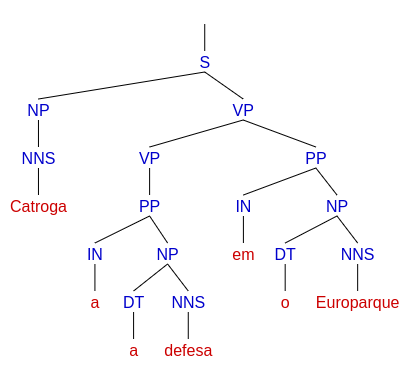
\includegraphics[width=\linewidth]{imagens/ec_cintil_sem_ponto_tree_trans.png}
        % \begin{forest}
        %     [
        %      [S 
        %       [NP 
        %       [NNS Catroga]
        %       ]
        %       [VP 
        %       [VP 
        %         [PP 
        %          [\textbf{IN a\_}]
        %          [NP 
        %           [\textbf{DT a}]
        %           [NNS defesa]
        %          ]
        %         ]
        %       ]
        %       [PP 
        %         [\textbf{IN em\_}]
        %         [NP 
        %          [\textbf{DT o}]
        %          [NNS Europarque]
        %         ]
        %       ]
        %       ]
        %      ]
        %     ]
        % \end{forest}
    \end{minipage}
    % 
    \begin{minipage}{.45\textwidth}
        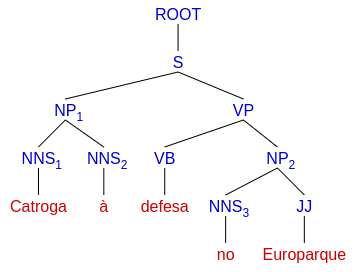
\includegraphics[width=\linewidth]{imagens/ec_cintil_sem_ponto_tree_sp.png}
        % \begin{forest}
        %     [ROOT
        %       [S
        %         [NP [NNS Catroga] [\textbf{JJ à}]]
        %         [VP [VB defesa]
        %           [NP [\textbf{NNS no}] [JJ Europarque]]]]]
        % \end{forest}
    \end{minipage}
    \caption[Estudo de caso CINTIL - Sentença transduzida sem pontuação]{Estudo da sentença eCTMP-000647/78121, \textquote{Catroga à defesa no Europarque}, que originalmente não possui nenhuma pontuação}
    \label{fig:ec_cintil_sem_ponto_tree}
\end{figure}
\end{center}

Na Figura \ref{fig:ec_cintil_sem_ponto_tree}, vemos o resultado da classificação de uma sentença originalmente sem pontuações. Há algumas coisas interessantes a serem notadas. Se, por um lado, de fato a falta de pontuação ajudou no \textit{parsing}, 
% por outro o SP tem dificuldades em separar contrações de preposições.
as contrações de preposição (\textquote{à}, \textquote{no}) não são identificados. O que faz sentido, pois o treino foi feito considerando tais separações.

\begin{center}
    \begin{figure}[!ht]
    \centering
    a)
    \begin{minipage}{.45\textwidth}
        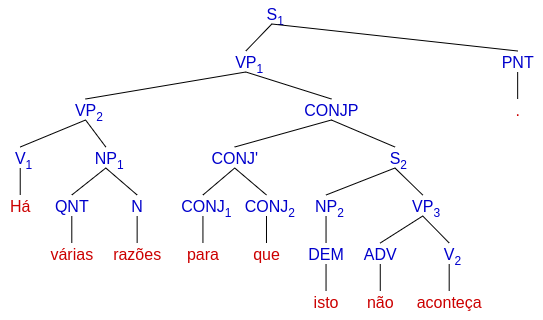
\includegraphics[width=\linewidth]{imagens/ec_cintil_conjp_tree_orig.png}
    \end{minipage}
    \hfill
    b)
    \begin{minipage}{.45\textwidth}
        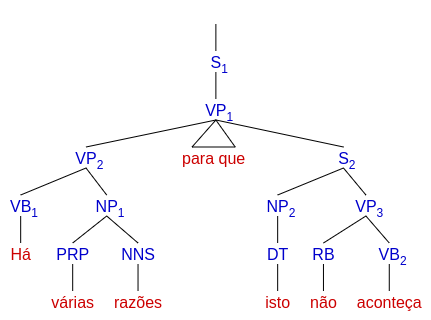
\includegraphics[width=\linewidth]{imagens/ec_cintil_conjp_tree_trans.png}
    \end{minipage}
    \hfill
    \vskip\floatsep
    c)
    \begin{minipage}{.45\textwidth}
        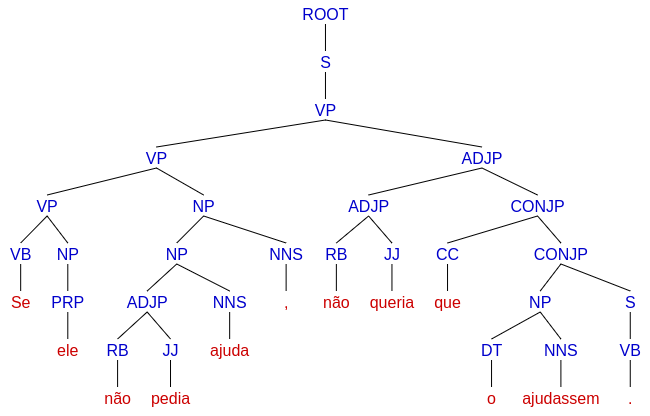
\includegraphics[width=\linewidth]{imagens/ec_cintil_conjp_tree_sp.png}
    \end{minipage}
    \caption[Estudo de caso CINTIL - Árvore da sentença transduzida com CONJP]{Estudo da sentença eCTMP-001150/117736, \textquote{Há várias razões para que isto não aconteça.}, que possui CONJP internamente. Em a), temos a árvore como se apresenta originalmente no CINTIL. Em b), temos a mesma sentença, pós transdução. Em c), temos o resultado da classificação do SP, utilizando a gramática gerada neste trabalho (após o processo de transdução)}
    \label{fig:ec_cintil_conjp_tree}
\end{figure}
\end{center}

A Figura \ref{fig:ec_cintil_conjp_tree} nos dá mais material de interesse. 
% Por exemplo, pode-se notar como a ausência de conhecimento de léxico da língua classificada gera confusões. 
% O \textquote{o} é facilmente confundido, mas não apenas. 
% O sintagma CONJP, que some na árvore transduzida, retorna na árvore classificada. Interessante notar que a 
% que a transforma num adjunto de VP. 
% O sintagma VP, em \textquote{não podia} tem seu núcleo, e por conseguinte, o sintagma como um todo, alterado. Provavelmente, para seguir a tendência da língua inglesa, que costuma ter o núcleo do sintagma posicionado mais à direita \cite[p~40]{charniak97statistical}. 
% A confusão com as pontuações é notável, sendo transformadas em substantivo (NNS) ou verbo (VB), o que é curioso. 
% Supões-se que o SP não seja estranho à pontuações mesmo que elas não venham no seu conjunto de treino.
A confusão gerada pela falta de treinamento sobre pontuações permanece, sendo ainda uma das maiores falhas. O $VP_3$ \textquote{não aconteça} se torna um $ADJP$, considerando como núcleo o advérbio \textquote{não}. O esforço de manter a estrutura de conjunções, que estudamos na Seção \ref{subsec-cintil-conj} é desfeito, convertendo o sintagma solto em \textit{flat structure} \textquote{para que} se converte num PP. Vale notar que ele não se torna um sintagma conjuntivo (CONJP), e \textquote{que} não é marcado como CC, que é a tendência tradicional do \textit{parser}. Também, apesar da tendência da língua inglesa, que costuma ter o núcleo do sintagma posicionado mais à direita \cite[p~40]{charniak97statistical}, isso não ocorre nem no PP, nem no ADJP.

\begin{center}
    \begin{figure}[!ht]
    \centering
    \begin{minipage}{.45\textwidth}
        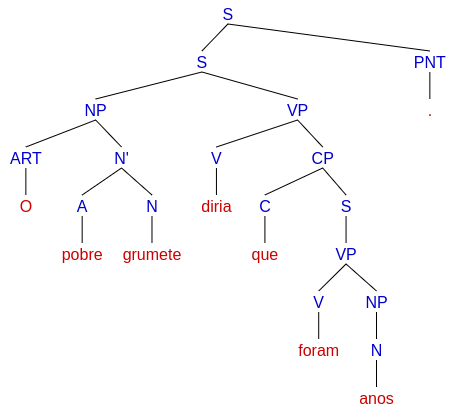
\includegraphics[width=\linewidth]{imagens/ec_cintil_cp_tree_orig.png}
        \caption{árvore original}
    \end{minipage}
    \hfill
    \begin{minipage}{.45\textwidth}
        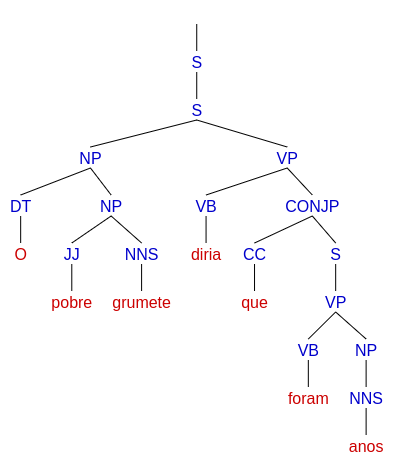
\includegraphics[width=\linewidth]{imagens/ec_cintil_cp_tree_trans.png}
        \caption{árvore transduzida}
    \end{minipage}
    \hfill
    \vskip\floatsep
    \begin{minipage}{.45\textwidth}
        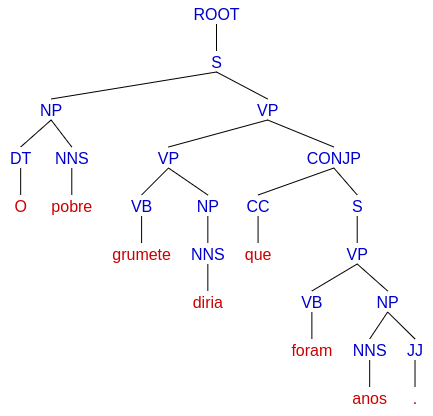
\includegraphics[width=\linewidth]{imagens/ec_cintil_cp_tree_sp.png}
        \caption{árvore gerada pelo SP}
    \end{minipage}
    \caption[Estudo de caso CINTIL - Árvore da sentença transduzida com CP]{Estudo da sentença eCTMP-000694/81773, \textquote{O pobre grumete diria que foram anos.}, que possui CP internamente.}
    \label{fig:ec_cintil_cp_tree}
\end{figure}
\end{center}

Verificando as alterações realizadas sobre o sintagma CP, como vimos na Seção \ref{subsec-cintil-c}, vejamos a Figura \ref{fig:ec_cintil_cp_tree}. Curiosamente, o sintagma em questão está acompanhando bem a estrutura da árvore original, e da árvore transduzida. 
% O maior destaque ficam para as palavras de classe aberta (substantivos, verbos, adjetivos). Aparentemente, a informação léxica continua sendo um problema.
\begin{center}
    \begin{figure}[!ht]
    \centering
    \begin{minipage}{.45\textwidth}
        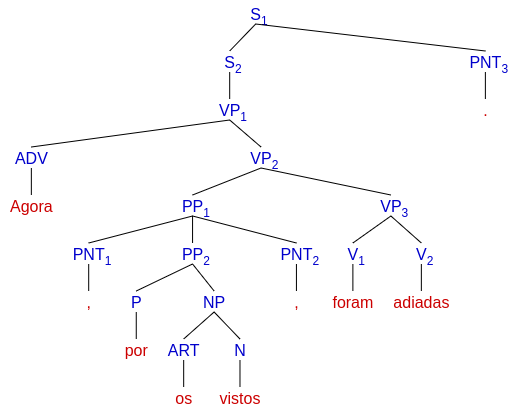
\includegraphics[width=\linewidth]{imagens/ec_cintil_virgula_tree_orig.png}
        \caption{árvore original}
    \end{minipage}
    \hfill
    \begin{minipage}{.45\textwidth}
        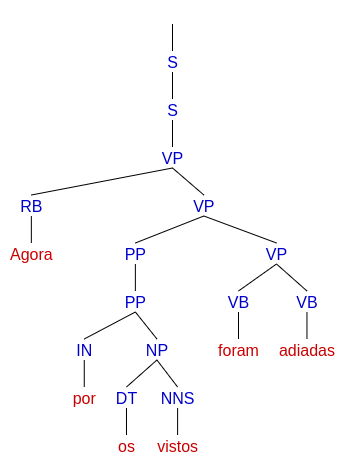
\includegraphics[width=\linewidth]{imagens/ec_cintil_virgula_tree_trans.png}
        \caption{árvore transduzida}
    \end{minipage}
    \hfill
    \vskip\floatsep
    \begin{minipage}{.45\textwidth}
        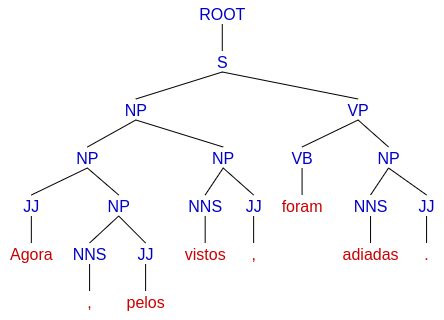
\includegraphics[width=\linewidth]{imagens/ec_cintil_virgula_tree_sp.png}
        \caption{árvore gerada pelo SP}
    \end{minipage}
    \caption[Estudo de caso CINTIL - Árvore da sentença transduzida com vírgulas]{Estudo da sentença eCTMP-001597/153293, \textquote{Agora, pelos vistos, foram adiadas.}, que possui vírgulas.}
    \label{fig:ec_cintil_virgula_tree}
\end{figure}
\end{center}

Para finalizar nossa revisão com as transduções do CINTIL, temos a Figura \ref{fig:ec_cintil_virgula_tree}, a respeito da colocação de vírgulas.
Pode-se notar a dificuldade léxica, onde palavras como \textquote{vistos} e \textquote{adiadas} são confundidos. Acredita-se que, se a contração da palavra \textquote{pelos} fosse detectada, a presença do Determinante resolveria tal problema. Os erros de marcação destes terminais afetam toda a marcação da árvore acima. Curioso notar também que, sem o treino de pontuações, tais símbolos se tornam ou substantivos (NNS), ou adjetivos (JJ). Porém, nem sempre são marcadas da mesma maneira, como pode ser comparado entre as Figuras \ref{fig:ec_cintil_virgula_tree} e \ref{fig:ec_cintil_conjp_tree}.
% Nota-se uma tendência muito interessante, do SP, de considerar palavras como adjetivo (JJ). Mesmo para palavras que nunca assumem tal forma, como \textquote{pelos}, que pode ser ou a contração \textit{por + os}, ou um substantivo. A falta de treinamento com pontuações mais uma vez é sentida, uma vez que SP não sabe como resolver vírgulas e pontos.
\subsection{Resultados do Bosque}
\label{subsec:resultados_bosque}
Neste momento, serão mostrados os resultados das execuções baseadas no BOSQUE.

\subsubsection{Treinamento} 
\label{subsubsec:result_treino_bosque}
Na Tabela \ref{tab:resultados_treino_bosque}, vemos os resultados dos treinamentos do SP sobre Bosque transduzido por nós. Note que os campos são equivalentes aos explicados em \ref{result_treino_cintil}.
\begin{center}
    \begin{table}[h!]
    \centering
    % \begin{tabular}{|l|c|c|c|c|c|c|}
    % \hline
    %     Grammar & States & Tags & Words & UnaryR & BinaryR & Taggings\\
    %     \hline
    %     1 & 482 & 15 & 2881 & 59 & 1182 & 2948\\
    %     2 & 496 & 16 & 2627 & 66 & 1170 & 2679\\
    %     3 & 527 & 16 & 2845 & 52 & 1206 & 2902\\
    %     4 & 505 & 17 & 2779 & 67 & 1188 & 2841\\
    %     5 & 480 & 16 & 2649 & 59 & 1166 & 2705\\
    %     6 & 487 & 16 & 2847 & 53 & 1190 & 2900\\
    %     7 & 472 & 15 & 2774 & 54 & 1192 & 2825\\
    %     8 & 477 & 17 & 2823 & 66 & 1192 & 2889\\
    %     9 & 522 & 18 & 2718 & 64 & 1183 & 2778\\
    %     10 & 404 & 16 & 2559 & 50 & 1027 & 2614\\
    %     \hline
    % \end{tabular}
    \csvautotabular{tabelas/resultados-bosque-treino.csv}
    \caption[Resultados do treinamento do Bosque]{Resultados dos treinamentos do Bosque, para os 10 \textit{folds}}
    \label{tab:resultados_treino_bosque}
\end{table}
\end{center}

A Figura \ref{fig:treino_bosque} nos dá a visualização desses resultados. Pode-se observar que o resultado pre-eliminar dos testes é muito superior ao visualizado em \ref{result_treino_cintil}.
\begin{center}
    \begin{figure}[!ht]
    \centering
    % \includegraphics{}
    \includesvg[width=.8\textwidth]{imagens/treino_bosque}
    % \includesvg{imagens/bosque_pcfg}
    \caption[Gráfico de resultados do treinamento, usando o BOSQUE transduzido]{Gráfico de resultados do treinamento do LexicalizedParser, usando o BOSQUE transduzido}
    \label{fig:treino_bosque}
\end{figure}
\end{center}

\subsubsection{Avaliação} 
\label{subsubsec:result_aval_bosque}
Na Tabela \ref{tab:result_bosque_pcfg}, vemos o resultados dos testes utilizando o SP sobre o Bosque transduzido.
\begin{center}
    \begin{table}[!h]
    \centering
    \begin{tabular}{|l|c|c|c|}
        \hline
        % pcfg LP/LR summary evalb    &   LP  & LR    &   F1\\
        pcfg LP/LR & LP & LR & F1\\
        \hline
        fold 1 & 51.61 & 47.9 & 49.69\\
        fold 2 & 51.78 & 47.68 & 49.64\\
        fold 3 & 49.25 & 45.65 & 47.38\\
        fold 4 & 52.55 & 49.05 & 50.74\\
        fold 5 & 51.03 & 46.05 & 48.41\\
        fold 6 & 52.8 & 49.15 & 50.91\\
        fold 7 & 48.86 & 45.21 & 46.97\\
        fold 8 & 50.1 & 45.81 & 47.86\\
        fold 9 & 52.28 & 48.49 & 50.32\\
        fold 10 & 55.37 & 51.91 & 53.59\\
        \hline
    \end{tabular}
    % \csvautotabular{resultados-cintil-testes-pcfg.csv}
    \caption{Resultados do treinamento da PCFG do SP, usando dados do BOSQUE}
    \label{tab:result_bosque_pcfg}
\end{table}
% fold 1   &   44.6    &   41.62   &   43.06\\
% fold 2   &   44.15   &   41.48   &   42.78\\
% fold 4   &   44.52   &   41.4   &   42.9\\
% fold 5   &   44.17   &   41.56   &   42.82\\
% fold 6   &   44.29   &   41.02   &   42.59\\
% fold 7   &   44.92   &   42.14   &   43.49\\
% fold 8   &   44.83   &   41.62   &   43.17\\
% fold 9   &   43.88   &   40.83   &   42.3\\
% fold 10   &   43.78   &   40.54   &   42.1\\
\end{center}

A média da \textit{F1-Score} é de 49.551\%, e tem o desvio padrão de aprox. 1.992\%.

Na Figura \ref{fig:bosque_result_pcfg} podemos ter uma visualização melhor de tais resultados.
\begin{center}
    \begin{figure}[!ht]
    \centering
    % \includegraphics{}
    \includesvg[width=.8\textwidth]{imagens/bosque_pcfg}
    % \includesvg{imagens/cintil_pcfg}
    \caption[Gráfico de resultados dos testes usando o BOSQUE transduzido]{Gráfico de resultados dos testes do PCFG do LexicalizedParser, usando o BOSQUE transduzido}
    \label{fig:bosque_result_pcfg}
\end{figure}
\end{center}

É possível notar que, mesmo com o desempenho de treinamento melhor que os do CINTIL (como visto em \ref{result_treino_cintil}), a classificação continua tendo uma qualidade baixa. 
% nunca superando os 50\%.
Apenas os dois últimos \textit{folds} superam os 50\%.

\subsubsection{Estudos de caso}
\label{subsec:ec-bosque}

De modo análogo ao do CINTIL, vamos revisar aqui alguns casos curiosos de sentenças classificadas. Utilizaremos a gramática do décimo treino para as classificações e avaliações. O Bosque tem mais casos problemáticos que o CINTIL, e visualizar todas elas tornaria este trabalho ainda maior. Portanto, alguns casos serão exibidos apenas nos Apêndices.
\begin{center}
    \begin{figure}[!ht]
    \centering
    % \includegraphics{}
    \begin{minipage}{.45\textwidth}
        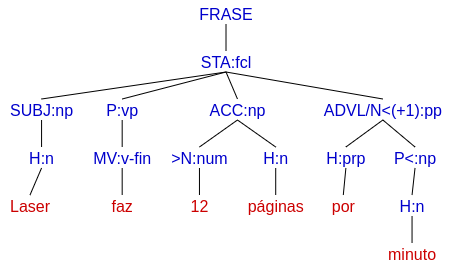
\includegraphics[width=\linewidth]{imagens/ec_bosque_sem_ponto_tree_orig.png}
        \caption{árvore original}
    \end{minipage}
    % 
    \begin{minipage}{.45\textwidth}
        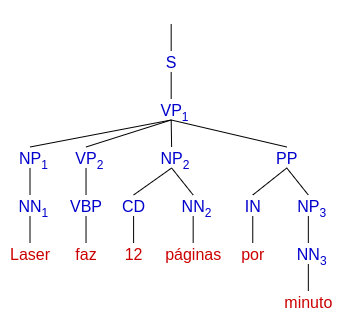
\includegraphics[width=\linewidth]{imagens/ec_bosque_sem_ponto_tree_trans.png}
        \caption{árvore transduzida}
    \end{minipage}
    \begin{minipage}{.45\textwidth}
        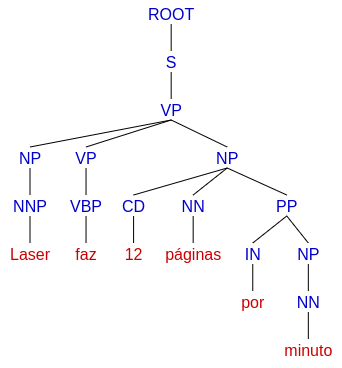
\includegraphics[width=\linewidth]{imagens/ec_bosque_sem_ponto_tree_sp.png}
        \caption{árvore gerada pelo SP}
    \end{minipage}
    \caption[Estudo de caso BOSQUE - Sentença transduzida sem pontuação]{Estudo da sentença CF761-1, \textquote{Laser faz 12 páginas por minuto}, que originalmente não possui nenhuma pontuação}
    \label{fig:ec_bosque_sem_ponto_tree}
\end{figure}
\end{center}

A Figura \ref{fig:ec_bosque_sem_ponto_tree} nos mostra as diferenças entre árvores sem pontuação. Foram removidas as informações adicionais dos nós da árvore original do Bosque, mantendo apenas $(F:f)$.
Temos poucos erros de \textit{parsing}. Nenhum nó terminal foi classificado erroneamente, apenas nós internos (não-terminais). Uma ambiguidade no $NP$ de \textquote{12 páginas}, que agora abarca também o $PP$ irmão. 
% E o núcleo do primeiro $NP$, que foi classificado como $NP$.

\begin{center}
    \begin{figure}[!hb]
    \centering
    % \includegraphics{}
    \begin{minipage}{.45\textwidth}
        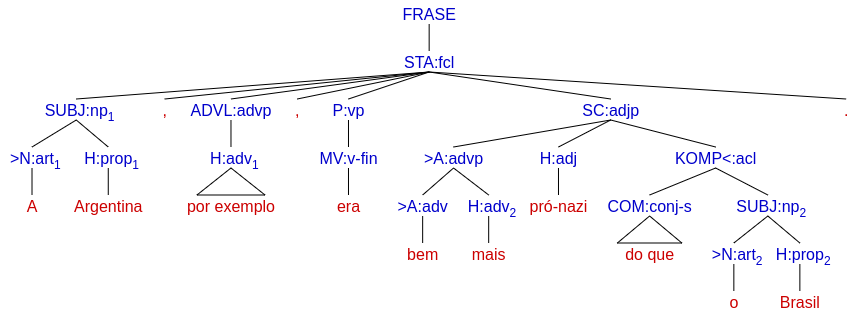
\includegraphics[width=\linewidth]{imagens/ec_bosque_komp_tree_orig.png}
        \caption{árvore original}
    \end{minipage}
    % 
    \begin{minipage}{.45\textwidth}
        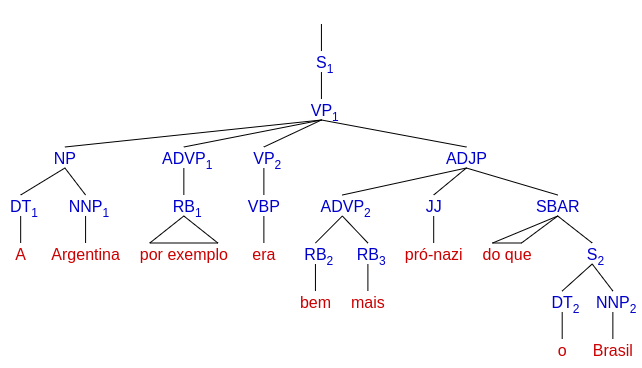
\includegraphics[width=\linewidth]{imagens/ec_bosque_komp_tree_trans.png}
        \caption{árvore transduzida}
    \end{minipage}
    \begin{minipage}{.45\textwidth}
        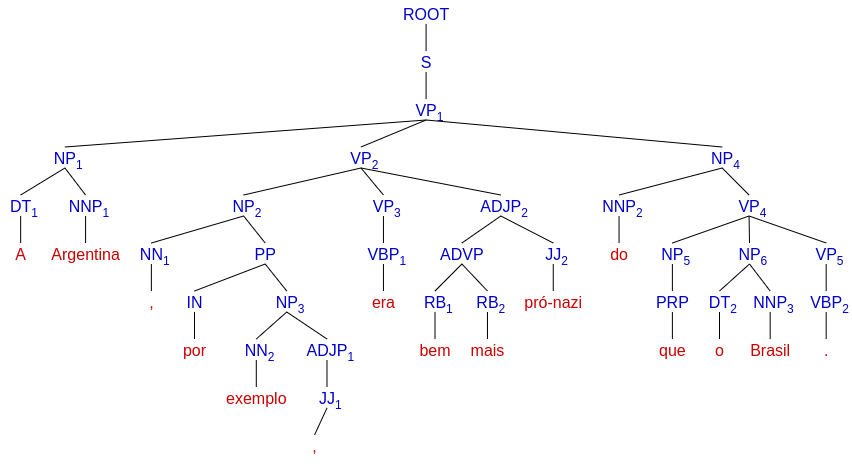
\includegraphics[width=\linewidth]{imagens/ec_bosque_komp_tree_sp.png}
        \caption{árvore gerada pelo SP}
    \end{minipage}

    \caption[Estudo de caso BOSQUE - Sentença transduzida com KOMP<:acl]{Estudo da sentença CF766-10, \textquote{A Argentina, por exemplo, era bem mais pró-nazi do que o Brasil.}, que possui a estrutura KOMP<:acl internamente.}
    \label{fig:ec_bosque_komp_tree}
\end{figure}
\end{center}

A Figura \ref{fig:ec_bosque_komp_tree} traz uma sentença que, originalmente, possui o par $KOMP<:acl$ internamente. É notório como as regras unárias (Não-terminal $\rightarrow$ terminal) são mais consistentes que as binárias. Curioso também a separação de palavras originalmente conjuntas, como \textquote{por exemplo} e \textquote{do que}. Ambas expressões aparecem pouco no CETEMFolha (22 e 34 vezes, respectivamente). Porém, pelas observações anteriores, supõe-se que o SP não está pronto para lidar com nós terminais concatenados durante a execução. 
% Cabe observar que a estrutura de Comparação foi mantida no estilo PTB, como visto em \ref{fig:ec_bosque_komp_detalhe}, apesar da discordância entre $SBAR$ (transdução) e $PP$ (\textit{Stanford}).
Interessante notar que a estrutura de Comparação (estudada em \ref{subsec:tag_komp}) foi desfeita pelo SP.

\begin{center}
    \begin{figure}[!hb]
    \centering
    % \includegraphics{}
    % \begin{subfigure}[t]{0.5\textwidth}
    \begin{minipage}{.45\textwidth}
        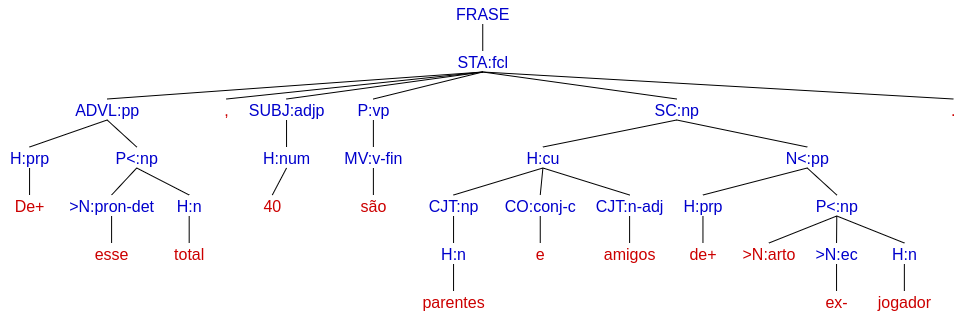
\includegraphics[width=\linewidth]{imagens/ec_bosque_ec_tree_orig.png}
        \caption{árvore original}
    % \end{subfigure}
    \end{minipage}
    % 
    \begin{minipage}{.45\textwidth}
        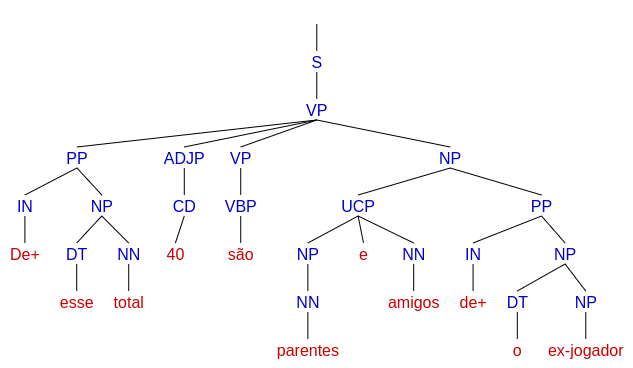
\includegraphics[width=\linewidth]{imagens/ec_bosque_ec_tree_trans.png}
        \caption{árvore transduzida}
    \end{minipage}
    \begin{minipage}{.45\textwidth}
        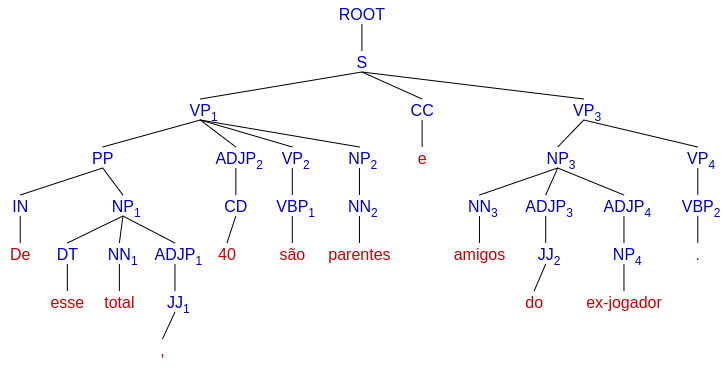
\includegraphics[width=\linewidth]{imagens/ec_bosque_ec_tree_ps.png}
        \caption{árvore gerada pelo SP}
    \end{minipage}
    % \begin{minipage}{.45\textwidth}
    %     \ldots
    %     \begin{tabbing}
    %         \=(NP\= (JJ ,) (NN Dawn)\+\\
    %         \>  (AD\=JP (JJ Upshaw)))\-\\
    %         \>(CC e)\\
    %         \>(VP\=\+\\
    %         \>  (VP (VBP Galina))\\
    %         \>  (NP\= (NN Gorchakova)\+\\
    %         \>      (ADJP (JJ .))))))))
    %     \end{tabbing}
    % \end{minipage}
    \caption[Estudo de caso BOSQUE - Sentença transduzida com \textit{ec}, e \textit{cu}]{Estudo da sentença CF866-2, \textquote{De esse total, 40 são parentes e amigos do ex-jogador.}, que possui a \textit{tag} \textit{ec}.}
    \label{fig:ec_bosque_ec_tree}
\end{figure}
\end{center}

A Figura \ref{fig:ec_bosque_ec_tree}
% vem com uma novidade inusitada: Foi considerada agramatical pelo \textit{parser} fatorado, disponibilizado pelo SP (que não abordamos neste trabalho). Mas foi interpretado pelo PCFG. 
traz um fato inesperado: a ideia com esta sentença era estudar a aplicação da \textit{tag} \textit{ec}, que inclusive não apresentou problemas. Mas a conjunção \textquote{parentes e amigos} foi desfeita pelo SP. \textquote{E} se tornou um mero irmão dos dois sintagmas, tal qual uma vírgula, e recebeu a \textit{tag} $CC$, que pouco aparece devido às conversões feitas na transdução para que o $SP$ aceitasse conjunções. O mesmo ocorre no \textit{parsing} da sentença CF318-C (fragmento em \ref{fig:ec_bosque_komp_detalhe}), mostrando que, apesar deste trabalho ter se guiado pelo \textit{Bracketing Guidelines} \cite{bracketing_ptb}, algumas estruturas poderiam se manter equivalentes às apresentadas no Bosque.

Outras análises serão apresentadas nos apêndices.
\subsection{Comentários}
\label{subsec:result_coment}

Fica claro, pela observação dos dados abordados, que a transdução de \textit{datasets} pode não ser o melhor caminho para suprir a necessidade de \textit{parsers} para o Português. Porém, existem algumas considerações que precisam ser feitas.

Primeiramente, deve-se notar como é curioso que, apesar do treino do SP com dados transduzidos pelo CINTIL possuírem uma maior quantidade de dados, os resultados do treino deste (visto na Tabela \ref{tab:resultados_treino_cintil}) são bastante tímidos, se comparados com os números da mesma operação sobre o Bosque (Tabela \ref{tab:resultados_treino_bosque}). Podemos levantar algumas hipóteses: 
\begin{itemize}
    \item A maior quantidade de dados permitiu que o SP tivesse mais acesso à árvores problemáticas, fazendo com que o resultado geral fosse inferior;
    \item Apesar do tamanho do Bosque ser menor, suas árvores são mais completas, permitindo maior generalização;
    \item A transdução dos dados do Bosque foi feita de forma mais acurada, permitindo um treinamento melhor.
\end{itemize}
É curioso notar, por exemplo, como o SP registrou mais \textit{tags} sobre o Bosque do que sobre o CINTIL. Observar as Tabelas \ref{tab:tab_cintil} e \ref{tab:tab_bosque} poderia ser uma alternativa, mas não se justifica: Foram usadas 20 \textit{tags} na transdução do Bosque, contra\ldots 20 do CINTIL. Mesmo com as duas tabelas de possibilidades do Bosque, para alguns casos (como comentado em \ref{subsec:sec_x} \ref{subsec:tag_acl}). A quantidade de regras gramaticais apreendidas quando nos baseamos no Bosque, também, é de um contraste muito interessante: no melhor caso do treinamento sobre CINTIL (\textit{fold 1}), foram aprendidas 257 regras, contra 1027 do pior caso do treino com o Bosque (\textit{fold 10}). Observar as Figuras \ref{fig:treino_cintil} e \ref{fig:treino_bosque} nos permite ver essas diferenças.

Uma olhada mais atenta às \textit{tags} utilizadas pode nos dar uma pista. Como pode-se ver na Tabela \ref{tab:comp_cintil_bosque}, basicamente foram usadas as mesmas \textit{tags}. As diferenças expressivas estão, no CINTIL, no uso repetitivo das interjeições, e no uso de CONJP. Bosque, por outro lado, tem uma pluralidade maior de marcações relativas à verbos. Retornar à Tabela \ref{tab:tab_bosque} nos faz ver que tal característica vem desde o \textit{treebank} original. 
\begin{center}
    \begin{table}[!h]
    \centering
    \begin{tabular}{|l|l|}
        \hline
        CINTIL  &   BOSQUE\\
        \hline
        ADVP    &   ADJP\\
        ADJP    &   ADVP\\
        CC    & CC\\
        CD    &  CD\\
        CONJP    & DT\\
        DT    & IN\\
        IN    & JJ\\
        INTJ    &   NN\\
        JJ    & NP\\
        NN    & NNP\\
        NNS    &    PP\\
        NP    & PRP\\
        PP    & RB\\
        PP\$    &    S\\
        PRP    &   UH\\
        RB    & VB\\
        S    &  VBP\\
        UH    & VBG\\
        VB    & VP\\
        VP    & VBN\\
        \hline
    \end{tabular}
    \caption[Tags utilizadas nas transduções do CINTIL e do Bosque]{Tags utilizadas nas transduções do CINTIL e do Bosque}
    \label{tab:comp_cintil_bosque}
\end{table}
\end{center}

Seria o caso, então, de uma maior atenção no desenvolvimento da solução para um \textit{dataset} do que para o outro? Pode-se afirmar que não. Toda alteração feita, como já dito ao longo do trabalho, foi com o objetivo de fazer com que o \textit{Stanford Parser} fosse capaz de receber as florestas sintáticas transduzidas. Toda alteração e desenvolvimento foram feitos pensando no mínimo necessário para que o processamento fosse possível. Com isso, quer-se dizer que: A ambos conjuntos de dados, foi dada atenção equivalente.
% pois o objetivo deste trabalho não era fazer uma adaptação perfeita. 
Código foi escrito na medida que o SP, e os \textit{treebanks} \textquote{exigiam}.
% Para citar um fato, em \ref{subsec:percent} comentamos que precisamos excluir as sentenças que incluíam \textquote{\%} em seu corpo. Isso dá um total de 149 sentenças, aprox. 3,5\% do \textit{dataset} completo.
\begin{center}
    \begin{figure}[!ht]
    \centering
    \includesvg[width=.8\textwidth]{imagens/comparativo_F1-Score_CINTIL_Bosque}
    \caption[Comparativo entre resultados de \textit{F1-Score}]{Comparativo entre resultados de \textit{F1-Score} para os 10 \textit{folds} do CINTIL e do Bosque}
    \label{fig:comp_f1_cintil_bosque}
\end{figure}
\end{center}
O que nos leva a um novo problema: ambos \textit{datasets} tiveram resultados baixos de \textit{F1-score}, variando entre 41\% e 45\%. A Figura \ref{fig:comp_f1_cintil_bosque} permite melhor visualização.
% Tal fato também nos faz levantar algumas hipóteses.
As seções \ref{result_aval_cintil} e \ref{result_aval_bosque} nos fazem entender o motivo. O mesmo conjunto de dados foi usado tanto para o treino como para os testes. Porém, ao executar sentenças reais, os resultados são sofríveis. Deve-se levar em consideração os pontos abordados sobre as características da métrica de avaliação em \ref{subsec:parseval}, é claro. Mas é inegável: os \textit{parse} obtidos estão muito aquém do esperado. 

A observação mais próxima desses resultados indica uma possível resposta: o \textit{Stanford Parser} está muito atrelado às regras lexicais do Inglês. O que faz todo sentido, quando lembramos que deliberadamente optamos por usar tal \textit{parser}. Mais: ao optar-se por não fazer grandes desenvolvimentos a partir dele, ou até mesmo não utilizar modelos de outras linguagens que estão disponíveis e distribuídos oficialmente, era sabido que o modelo padrão que compõe o SP é o da língua inglesa. Portanto, em nada otimizado para o português, qualquer variante que seja. 

Faz todo o sentido retomar este trabalho no futuro, aprimorar suas características, e torná-lo mais preciso, sem que seja necessário descartar nenhuma sentença que seja. A ausência de pontuações é muito sentida no \textit{score} final. Mas, estamos convencidos: Transdutores não são a solução para o problema da ausência de \textit{parsers} para o Português.

Ou melhor, não sozinhos. Transduzir os dois \textit{datasets}, de modo que o SP fosse capaz de processá-las foi um grande avanço. Isto torna uma potencial nova etapa possível, essa sim podendo ser a resposta: adaptar o SP para o Português. Produzir um novo modelo de linguagem para a ferramenta parece ser uma alternativa plausível.

Esta ideia não é nova, o LX-Parser (\citeonline{Branco2010OutOfTheBox} e \citeonline{silva-etal-2010-top}) foi desenvolvido justamente com este pensamento. Mas se encontra obsoleto. Além de que, foi necessário usar um novo \textit{dataset} no seu desenvolvimento. Criar transdutores que adaptem florestas sintáticas pré-existentes pode ser um avanço nesta parte do desenvolvimento. Isto, claro, se pensarmos num desenvolvimento já apoiado em ferramentas e bibliotecas pré-existentes. Desenvolver um \textit{parser} novo sempre é uma possibilidade.

Por fim, precisamos voltar à pergunta levantada em \ref{cha:introducao} e \ref{sec:contexto}: seria possível a alguém, com pouco conhecimento acadêmico, realizar tarefa semelhante ao do trabalho apresentado? A resposta é: Dificilmente. 

Desenvolver os transdutores exigiu uma certa gama de conhecimentos interessantes e multidisciplinares. Fora algumas necessidades. Ter um computador, por exemplo. Suponhamos que ela tenha um computador, e não seja estranha à equipamentos eletrônicos. Ela vai precisar aprender a programar. A linguagem de programação deste trabalho foi Python, que tem baixa dificuldade de aprendizado inicial. Ótimo começo. A pessoa em questão precisa saber o básico de manipulação de \textit{strings}, o que por sorte, costuma ser um dos aprendizados iniciais. As facilidades param por aí. Construir o transdutor exige o conhecimento de estruturas de dados, para que a estrutura simbólica das árvores seja reproduzida logicamente. Por conseguinte, é preciso também ser capaz de manipular tais árvores. Pode-se ter uma noção intuitiva disto, mas não é um assunto trivial. Também, exige que ela tenha conhecimento de árvores de constituência. Dependendo do histórico de vida desta pessoa, ela viu algo semelhante na escola. Mas é um conhecimento de cursos de licenciatura / bacharelado em letras. Também, o transdutor exige multidisciplinaridade do desenvolvedor. É preciso ter disposição para programar, assim como de ler gramáticas para estudar regras gramaticais e linguísticas. Não ter esses conhecimentos implicará em código ruim. 

Mais: me referi apenas à construção dos transdutores. Para a construção de \textit{parsers}, será necessário um bom conhecimento de estatística, e de desenvolvimento em inteligência artificial. Como mostramos em \ref{subsec:statisticalparsing}, nem só a estatística será suficiente para se obter um \textit{parser} utilizável.

Fica, então, a dúvida: uma pessoa que queira usar um \textit{parser} precisa mesmo de tudo isso? Bastaria usar os disponíveis. Mas, como já citado ao longo deste trabalho, existem poucos disponíveis. E \textit{parsers} podem ser úteis para o público geral. No aprendizado de línguas, nativa ou estrangeira, ou tradução, por exemplo. Se esta pessoa hipotética não conseguir achar algum \textit{parser} que lhe seja útil, ela seria capaz de construir um por conta própria?

A resposta otimista é: Esperamos que sim. Muito material de estudo está disponível gratuitamente e de forma acessível. A resposta pessimista é que sem bagagens prévias de conhecimento, será muito complicado. Boa sorte aos futuros desenvolvedores.
% ---
% Conclusão (outro exemplo de capítulo sem numeração e presente no sumário)
% ---
\chapter{Considerações Finais}
\label{chap:considFinal}
Neste trabalho, estudamos \textit{parsers}, suas limitações e possibilidades. Vimos que existem \textit{parsers} principalmente para a língua inglesa. Que há poucos para a língua portuguesa. Que existem conjuntos de dados em Português que podem ser usados para treinar \textit{parsers}. Propusemos, então, a transdução de dados estruturados em Português para o Inglês, sem perda de informação léxica, e realizamos tal transdução. Verificamos que, apesar de ser uma abordagem interessante, o trabalho em questão ainda não é uma solução, quando o problema é a baixa oferta de \textit{parsers} para a língua portuguesa.

Por fim, ficam algumas propostas de trabalhos futuros. Que conste:
A revisão deste trabalho, ampliando os casos tratados (por exemplo, quais situações são descritas não por \textit{POS tags}, mas pela \textit{estrutura} da árvore?);
a correção de estruturas que, para este trabalho, não estão em padrão aceitável, como sinais de pontuação, e a porcentagem da transdução do Bosque (\ref{subsec:percent});
o desenvolvimento de transdutores como alternativa ao desenvolvimento de \textit{parsers};
a implementação de \textit{parser}, com desenvolvimento \textit{out-of-the-box} para o português; 
dentre outras possibilidades. 

% ----------------------------------------------------------
% Finaliza a parte no bookmark do PDF
% para que se inicie o bookmark na raiz
% e adiciona espaço de parte no Sumário
% ----------------------------------------------------------
\phantompart
% ---

%texto vem aqui

% ----------------------------------------------------------
% ELEMENTOS PÓS-TEXTUAIS
% ----------------------------------------------------------
\postextual
% ----------------------------------------------------------
\begin{apendicesenv}
\partapendices

\chapter{CINTIL}
\label{ap_cintil}

\section{Tabelas}
\label{ap_cintil_tab}

\begin{center}
    \begin{longtable}{|p{0.4\textwidth}|p{0.1\textwidth}|p{0.1\textwidth}|p{0.1\textwidth}|p{0.1\textwidth}|p{0.1\textwidth}|}
\caption{Tabela com resultados completos do CINTIL}\\
\hline
 & \textbf{LP} & \textbf{LR} & \textbf{F1} & \textbf{Exact} & \textbf{N} \\
\hline
\endfirsthead
\multicolumn{6}{c}%
{\tablename\ \thetable\ -- \textit{Continuação da página anterior}} \\
\hline
 & \textbf{LP} & \textbf{LR} & \textbf{F1} & \textbf{Exact} & \textbf{N} \\
\hline
\endhead
\hline \multicolumn{6}{r}{\textit{Continua na próxima página}} \\
\endfoot
\hline
\endlastfoot
    % \csvautotabular{tabelas/resultados-cintil_testes.csv}
    1 & 	 & 	 & 	 & 	 & 		\\
    pcfg LP/LR summary evalb: &  58.09  &  65.99  &  61.79  &  27.46  &  863\\
    dep DA summary evalb:  &  69.47  &  69.47  &  69.47  &  34.26  &  858\\
    factor LP/LR summary evalb:  &  59.69  &  68.88  &  63.96  &  28.38  &  863\\
    factor Tag summary evalb:  &  81.94  &  82.78  &  82.36  &  54.92  &  863\\
    2 & 	 & 	 & 	 & 	 & 	\\
    pcfg LP/LR summary evalb:  &  62.52  &  62.32  &  62.42  &  18.27  &  93\\
    dep DA summary evalb:  &  70.69  &  70.69  &  70.69  &  24.73  &  93\\
    factor LP/LR summary evalb:  &  67.82  &  69.88  &  68.83  &  20.43  &  93\\
    factor Tag summary evalb:  &  85.89  &  86.35  &  86.12  &  38.7  &  93\\
    3 & 	 & 	 & 	 & 	 & 	\\
    pcfg LP/LR summary evalb:  &  55.69  &  54.58  &  55.13  &  15.0  &  100\\
    dep DA summary evalb:  &  67.4  &  67.4  &  67.4  &  24.0  &  100\\
    factor LP/LR summary evalb:  &  64.95  &  65.75  &  65.35  &  25.0  &  100\\
    factor Tag summary evalb:  &  83.63  &  83.96  &  83.79  &  36.0  &  100\\
    4 & 	 & 	 & 	 & 	 & 	\\
    pcfg LP/LR summary evalb:  &  54.03  &  51.31  &  52.63  &  13.79  &  87\\
    dep DA summary evalb:  &  70.44  &  70.44  &  70.44  &  29.88  &  87\\
    factor LP/LR summary evalb:  &  61.23  &  59.49  &  60.35  &  12.64  &  87\\
    factor Tag summary evalb:  &  85.37  &  85.37  &  85.37  &  35.63  &  87\\
    5 & 	 & 	 & 	 & 	 & 	\\
    pcfg LP/LR summary evalb:  &  61.48  &  64.64  &  63.02  &  23.17  &  82\\
    dep DA summary evalb:  &  63.81  &  63.81  &  63.81  &  24.39  &  82\\
    factor LP/LR summary evalb:  &  64.61  &  69.12  &  66.79  &  30.48  &  82\\
    factor Tag summary evalb:  &  84.94  &  84.94  &  84.94  &  40.24  &  82\\
    6 & 	 & 	 & 	 & 	 & 	\\
    pcfg LP/LR summary evalb:  &  58.81  &  57.61  &  58.21  &  14.49  &  69\\
    dep DA summary evalb:  &  69.88  &  69.88  &  69.88  &  27.53  &  69\\
    factor LP/LR summary evalb:  &  68.56  &  68.06  &  68.31  &  20.28  &  69\\
    factor Tag summary evalb:  &  85.97  &  86.35  &  86.16  &  36.23  &  69\\
    7 & 	 & 	 & 	 & 	 & 	\\
    pcfg LP/LR summary evalb:  &  62.51  &  63.67  &  63.09  &  25.33  &  75\\
    dep DA summary evalb:  &  74.13  &  74.13  &  74.13  &  36.0  &  75\\
    factor LP/LR summary evalb:  &  67.72  &  69.08  &  68.4  &  28.0  &  75\\
    factor Tag summary evalb:  &  88.09  &  88.09  &  88.09  &  44.0  &  75\\
    8 & 	 & 	 & 	 & 	 & 	\\
    pcfg LP/LR summary evalb:  &  53.03  &  54.05  &  53.54  &  16.41  &  67\\
    dep DA summary evalb:  &  68.04  &  68.04  &  68.04  &  26.86  &  67\\
    factor LP/LR summary evalb:  &  59.23  &  61.76  &  60.47  &  17.91  &  67\\
    factor Tag summary evalb:  &  85.65  &  85.65  &  85.65  &  35.82  &  67\\
    9 & 	 & 	 & 	 & 	 & 	\\
    pcfg LP/LR summary evalb:  &  61.76  &  57.5  &  59.56  &  21.11  &  90\\
    dep DA summary evalb:  &  67.12  &  67.12  &  67.12  &  26.96  &  89\\
    factor LP/LR summary evalb:  &  65.31  &  62.84  &  64.05  &  24.44  &  90\\
    factor Tag summary evalb:  &  86.35  &  86.35  &  86.35  &  45.55  &  90\\
    10 & 	 & 	 & 	 & 	 & 	\\
    pcfg LP/LR summary evalb:  &  63.32  &  63.98  &  63.65  &  20.89  &  67\\
    dep DA summary evalb:  &  65.9  &  65.9  &  65.9  &  28.35  &  67\\
    factor LP/LR summary evalb:  &  65.13  &  67.55  &  66.32  &  19.4  &  67\\
    factor Tag summary evalb:  &  84.63  &  85.01  &  84.82  &  40.29  &  67
    \label{tab:cintil_result_full}
\end{longtable}
    % 1 &  &  &  &  & \\
    % pcfg LP/LR summary evalb: & 45.43 & 45.04 & 45.24 & 11.23 & 730\\
    % dep DA summary evalb: & 57.22 & 57.22 & 57.22 & 18.24 & 729\\
    % factor LP/LR summary evalb: & 51.83 & 52.56 & 52.19 & 13.56 & 730\\
    % factor Tag summary evalb: & 74.71 & 74.87 & 74.79 & 18.76 & 730\\
    % 2 &  &  &  &  & \\
    % pcfg LP/LR summary evalb: & 42.87 & 46.27 & 44.5 & 4.26 & 1500\\
    % dep DA summary evalb: & 49.18 & 49.18 & 49.18 & 14.77 & 1448\\
    % factor LP/LR summary evalb: & 42.89 & 47.23 & 44.96 & 4.06 & 1500\\
    % factor Tag summary evalb: & 67.1 & 67.48 & 67.29 & 4.13 & 1500\\
    % 3 &  &  &  &  & \\
    % pcfg LP/LR summary evalb: & 39.8 & 42.86 & 41.27 & 3.54 & 1493\\
    % dep DA summary evalb: & 49.28 & 49.28 & 49.28 & 11.84 & 1478\\
    % factor LP/LR summary evalb: & 39.97 & 44.02 & 41.9 & 3.68 & 1493\\
    % factor Tag summary evalb: & 62.74 & 63.1 & 62.92 & 3.61 & 1493\\
    % 4 &  &  &  &  & \\
    % pcfg LP/LR summary evalb: & 43.55 & 47.44 & 45.42 & 4.18 & 1506\\
    % dep DA summary evalb: & 59.71 & 59.71 & 59.71 & 17.44 & 1364\\
    % factor LP/LR summary evalb: & 43.76 & 48.13 & 45.84 & 4.38 & 1506\\
    % factor Tag summary evalb: & 64.98 & 65.38 & 65.18 & 4.24 & 1506\\
    % 5 &  &  &  &  & \\
    % pcfg LP/LR summary evalb: & 41.82 & 43.7 & 42.74 & 4.1 & 1511\\
    % dep DA summary evalb: & 46.98 & 46.98 & 46.98 & 15.76 & 1484\\
    % factor LP/LR summary evalb: & 41.57 & 45.19 & 43.3 & 4.3 & 1511\\
    % factor Tag summary evalb: & 63.41 & 63.79 & 63.6 & 4.16 & 1511\\
    % 6 &  &  &  &  & \\
    % pcfg LP/LR summary evalb: & 41.24 & 43.26 & 42.23 & 3.47 & 1524\\
    % dep DA summary evalb: & 53.29 & 53.29 & 53.29 & 15.39 & 1507\\
    % factor LP/LR summary evalb: & 41.68 & 44.69 & 43.14 & 3.74 & 1524\\
    % factor Tag summary evalb: & 61.77 & 62.12 & 61.95 & 3.34 & 1524\\
    % 7 &  &  &  &  & \\
    % pcfg LP/LR summary evalb: & 44.51 & 45.43 & 44.97 & 6.65 & 1518\\
    % dep DA summary evalb: & 47.55 & 47.55 & 47.55 & 12.83 & 1449\\
    % factor LP/LR summary evalb: & 44.15 & 46.29 & 45.19 & 6.85 & 1518\\
    % factor Tag summary evalb: & 61.98 & 62.35 & 62.17 & 5.73 & 1518\\
    % 8 &  &  &  &  & \\
    % pcfg LP/LR summary evalb: & 41.61 & 44.06 & 42.8 & 4.71 & 1526\\
    % dep DA summary evalb: & 51.59 & 51.59 & 51.59 & 12.51 & 1494\\
    % factor LP/LR summary evalb: & 42.01 & 44.93 & 43.42 & 4.65 & 1526\\
    % factor Tag summary evalb: & 62.75 & 63.13 & 62.94 & 5.5 & 1526\\
    % 9 &  &  &  &  & \\
    % pcfg LP/LR summary evalb: & 38.85 & 44.39 & 41.43 & 3.12 & 1503\\
    % dep DA summary evalb: & 51.94 & 51.94 & 51.94 & 12.97 & 1464\\
    % factor LP/LR summary evalb: & 38.82 & 45.17 & 41.76 & 2.99 & 1503\\
    % factor Tag summary evalb: & 64.52 & 64.91 & 64.72 & 3.79 & 1503\\
    % 10 &  &  &  &  & \\
    % pcfg LP/LR summary evalb: & 39.92 & 44.13 & 41.92 & 2.88 & 1526\\
    % dep DA summary evalb: & 50.25 & 50.25 & 50.25 & 10.94 & 1325\\
    % factor LP/LR summary evalb: & 39.06 & 44 & 41.38 & 2.81 & 1526\\
    % factor Tag summary evalb: & 61.49 & 61.84 & 61.67 & 2.03 & 1526

% \begin{table}[h]
%     \centering
%     % \begin{tabular}{c|c}
%     %      &  \\
%     %      & 
%     % \end{tabular}
%     \csvautotabular{tabelas/resultados-cintil_testes.csv}
%     \caption{Tabela com resultados completos do CINTIL}
%     \label{tab:cintil_result_full}
% \end{table}
\end{center}

\section{Imagens}
\label{ap_cintil_imagens}
% --------------------------------------------------------------------
\chapter{BOSQUE}
\label{ap_bosque}

\section{Tabelas}
\label{ap_bosque_tab}

\begin{center}
    \begin{longtable}{|p{0.4\textwidth}|p{0.1\textwidth}|p{0.1\textwidth}|p{0.1\textwidth}|p{0.1\textwidth}|p{0.1\textwidth}|}
\caption{Tabela com resultados completos do BOSQUE}\\
\hline
 & \textbf{LP} & \textbf{LR} & \textbf{F1} & \textbf{Exact} & \textbf{N} \\
\hline
\endfirsthead
\multicolumn{6}{c}%
{\tablename\ \thetable\ -- \textit{Continuação da página anterior}} \\
\hline
 & \textbf{LP} & \textbf{LR} & \textbf{F1} & \textbf{Exact} & \textbf{N} \\
\hline
\endhead
\hline \multicolumn{6}{r}{\textit{Continua na próxima página}} \\
\endfoot
\hline
\endlastfoot
    1 &  & &  &  & \\
    pcfg LP/LR summary evalb & 44.6 & 41.62 & 43.06 & 6.82 & 3650\\
    dep DA summary evalb & 68.39 & 68.39 & 68.39 & 14.04 & 3646\\
    factor LP/LR summary evalb & 47.31 & 45.97 & 46.63 & 8.73 & 3650\\
    factor Tag summary evalb & 64.63 & 66.08 & 65.35 & 9.28 & 3650\\
    2 &  &  &  &  & \\
    pcfg LP/LR summary evalb & 43.75 & 40.77 & 42.21 & 6.95 & 3652\\
    dep DA summary evalb & 67.26 & 67.26 & 67.26 & 12.92 & 3651\\
    factor LP/LR summary evalb & 46.41 & 45.27 & 45.83 & 8.13 & 3652\\
    factor Tag summary evalb & 64.24 & 65.68 & 64.96 & 9.44 & 3652\\
    3 &  &  &  &  & \\
    pcfg LP/LR summary evalb & 44.15 & 41.48 & 42.78 & 8.5 & 3657\\
    dep DA summary evalb & 67.66 & 67.66 & 67.66 & 13.26 & 3650\\
    factor LP/LR summary evalb & 46.92 & 45.92 & 46.42 & 8.28 & 3657\\
    factor Tag summary evalb & 64.18 & 65.59 & 64.88 & 8.12 & 3657\\
    4 &  &  &  &  & \\
    pcfg LP/LR summary evalb & 44.52 & 41.4 & 42.9 & 7.64 & 3661\\
    dep DA summary evalb & 67.7 & 67.7 & 67.7 & 13.34 & 3657\\
    factor LP/LR summary evalb & 46.21 & 44.64 & 45.41 & 8.44 & 3661\\
    factor Tag summary evalb & 63.95 & 65.36 & 64.65 & 9.09 & 3661\\
    5 &  &  &  &  & \\
    pcfg LP/LR summary evalb & 44.17 & 41.56 & 42.82 & 8.5 & 3667\\
    dep DA summary evalb & 67.17 & 67.17 & 67.17 & 13.62 & 3663\\
    factor LP/LR summary evalb & 46.16 & 45.11 & 45.63 & 8.75 & 3667\\
    factor Tag summary evalb & 63.76 & 65.16 & 64.45 & 8.8 & 3667\\
    6 &  &  &  &  & \\
    pcfg LP/LR summary evalb & 44.29 & 41.02 & 42.59 & 7.54 & 3656\\
    dep DA summary evalb & 67.65 & 67.65 & 67.65 & 13.54 & 3654\\
    factor LP/LR summary evalb & 47.03 & 45.46 & 46.23 & 8.2 & 3656\\
    factor Tag summary evalb & 64.05 & 65.5 & 64.77 & 8.78 & 3656\\
    7 &  &  &  &  & \\
    pcfg LP/LR summary evalb & 44.92 & 42.14 & 43.49 & 8.23 & 3654\\
    dep DA summary evalb & 67.67 & 67.67 & 67.67 & 13.11 & 3652\\
    factor LP/LR summary evalb & 46.97 & 46.05 & 46.5 & 8.83 & 3654\\
    factor Tag summary evalb & 64.62 & 66.04 & 65.32 & 9.49 & 3654\\
    8 &  &  &  &  & \\
    pcfg LP/LR summary evalb & 44.83 & 41.62 & 43.17 & 8.68 & 3663\\
    dep DA summary evalb & 68.34 & 68.34 & 68.34 & 13.95 & 3661\\
    factor LP/LR summary evalb & 46.84 & 46.13 & 46.49 & 8.4 & 3663\\
    factor Tag summary evalb & 65.08 & 66.52 & 65.79 & 10.04 & 3663\\
    9 &  &  &  &  & \\
    pcfg LP/LR summary evalb & 43.88 & 40.83 & 42.3 & 7.49 & 3658\\
    dep DA summary evalb & 67.52 & 67.52 & 67.52 & 12.94 & 3654\\
    factor LP/LR summary evalb & 45.88 & 44.69 & 45.28 & 8.25 & 3658\\
    factor Tag summary evalb & 64.06 & 65.5 & 64.77 & 9.02 & 3658\\
    10 &  &  &  &  & \\
    pcfg LP/LR summary evalb & 43.78 & 40.54 & 42.1 & 8 & 3649\\
    dep DA summary evalb & 67.49 & 67.49 & 67.49 & 12.76 & 3644\\
    factor LP/LR summary evalb & 46.64 & 45.48 & 46.05 & 9.64 & 3649\\
    factor Tag summary evalb & 63.97 & 65.43 & 64.69 & 9.78 & 3649
    \label{tab:bosque_result_full}
\end{longtable}
\end{center}

\begin{center}
    \begin{longtable}{|p{0.15\linewidth}|p{0.2\linewidth}|p{0.15\linewidth}|p{0.15\linewidth}|p{0.25\linewidth}|}
\caption{Tabela de conversão completa: BOSQUE para PTB (Funções)}\\
\hline
\textbf{Tag Original (Português)} & \textbf{Nome da Tag} & \textbf{Tag Convertida} & \textbf{Ocorrências} & \textbf{Observações}\\
\hline
\endfirsthead
\multicolumn{5}{c}%
{\tablename\ \thetable\ -- \textit{Continuação da página anterior}} \\
\hline
\textbf{Tag Original (Português)} & \textbf{Nome da Tag} & \textbf{Tag Convertida} & \textbf{Ocorrências} & \textbf{Observações} \\
\hline
\endhead
\hline \multicolumn{5}{r}{\textit{Continua na próxima página}} \\
\endfoot
\hline
\endlastfoot

    \textgreater A & dependente em adjp ou advp (antecede o núcleo) & \textgreater A & 371 & Explicado em \ref{subsec:bosque_a}\\
    A\textless  & dependente em adjp ou advp (segue o núcleo) & A\textless & 272 & Explicado em  \ref{subsec:bosque_a}\\
    A\textless ARG & Estrutura não descrita em \citeonline{freitas2007biblia} & não convertida & 12 & \\
    A\textless arg & Estrutura não descrita em  \citeonline{freitas2007biblia}  & não convertida & 45 & \\
    ACC & objecto directo (incluindo alguns tipos de se) & depende da \textit{form\_tag} & 4315 & Explicado em \ref{subsec:tag_acl}\\
    ACC-PASS & função do clítico se numa oração passiva (partícula apassivante) & NP & 39 & Refere-se ao uso de pronomes clíticos numa sentença\\
    ADVL & adjunto adverbial & depende da form & 6032 & Explicado em \ref{subsec:tag_acl}\\
    ADVL/A< [+1] & ambiguidade adjunto adverbial / adjunto adjetival & não convertida & 2 & \\
    ADVL/ADVL[-3] & ambiguidade adjunto adverbial / adjunto adjetival & não convertida & 2 & \\
    ADVL/N< [+1] & ambiguidade adjunto adverbial / adjunto adnominal & não convertida & 70 & \\
    ADVL/N< [+2] & ambiguidade adjunto adverbial / adjunto adnominal & não convertida & 25 & \\
    ADVL/N< [+3] & ambiguidade adjunto adverbial / adjunto adnominal & não convertida & 5 & \\
    ADVL/PIV & ambiguidade adjunto adverbial / obj. ind. preposicional & não convertida & 1 & \\
    APP & aposição (do substantivo)  [epíteto de identidade] & NP & 212 & \\
    AUX & verbo auxiliar & VBP & 1271 & \\
    AUX\textless  & Em contexto de coordenção, partícula de ligação entre o auxiliar partilhado e verbos coordenados & VP & 2 & \\
    CJT & elemento conjunto & \_CJT\_ & 3945 & Explicado em \ref{subsec:CJT}\\
    CJT\&ACC & Coordenação de constituintes com funções diferentes & NP & 1 & Por observação de frequências\\
    CJT\&ADVL & Coordenação de constituintes com funções diferentes & PP & 3 & Por observação de frequências\\
    CJT\&PASS & Coordenação de constituintes com funções diferentes & PP & 1 & Por observação de frequências\\
    CJT\&PRED & Coordenação de constituintes com funções diferentes & ADJP & 2 & Por observação de frequências\\
    CMD & enunciado imperativo & S & 7 & \\
    CO & coordenador & não convertida & 1753 & \\
    COM & complementizador em estruturas de comparação (como, (do) que ) & não convertida & 118 & \\
    DAT & objecto indirecto pronominal (incluindo \textit{se} ) & NP & 37 & \\
    EXC & enunciado exclamativo & S & 36 & \\
    FOC & marcador de foco & ADJP & 44 & \\
    H & núcleo & depende da form & 40148 & Explicado em \ref{subsec:tag_acl} \\
    KOMP\textless  & complemento comparativo & \_KOMP\_ & 40 & Explicado em \ref{subsec:tag_komp}\\
    MV & verbo principal & VP & 7999 & \\
    \textgreater N & adjunto adnominal (antecede o núcleo) & NP & 14009 & Dobra do NP por adjunto, como visto em \citeonline[p~67]{mioto2013novo}\\
    N\textless  & adjunto adnominal (segue o núcleo) & NP & 9208 & Dobra do NP por adjunto, como visto em \citeonline[p~67]{mioto2013novo}\\
    N\textless /ADVL[-1] & ambiguidade adjunto adnominal / adjunto adverbial & não convertida & 3 & \\
    N\textless /ADVL[-2] & ambiguidade adjunto adnominal / adjunto adverbial & não convertida & 1 & \\
    N\textless /ADVL[-3] & ambiguidade adjunto adnominal / adjunto adverbial & não convertida & 1 & \\
    N\textless /N\textless [+1] & ambiguidade adjunto adnominal / adjunto adnominal [1 nivel] & não convertida & 2 & \\
    N\textless /N\textless [+2] & ambiguidade adjunto adnominal / adjunto adnominal [2 níveis] & não convertida & 20 & \\
    N\textless /N\textless [-2] & ambiguidade adjunto adnominal / adjunto adnominal [2 níveis] & não convertida & 1 & \\
    N\textless /P\textless [+1] & ambiguidade adjunto adnominal / argumento de preposição & não convertida & 1 & \\
    N\textless ARG & complemento nominal (complementa um substantivo não deverbal) & PP & 139 & \\
    N\textless ARGO & complemento nominal (complementa um substantivo deverbal, relativo ao objecto) & PP & 450 & \\
    N\textless ARGS & complemento nominal (complementa um substantivo deverbal, relativo ao sujeito) & PP & 132 & \\
    N\textless PRED & adjeto predicativo [epíteto predicativo] & NP & 1542 & \\
    N\textless PRED / N\textless PRED[+2] & ambiguidade adjeto predicativo / adjeto predicativo & não convertida & 2 & \\
    N\textless PRED / N\textless PRED[-2] & ambiguidade adjeto predicativo / adjeto predicativo & não convertida & 1 & \\
    N\textless PRED / UTT[-4] & ambiguidade adjeto predicativo / enunciado & não convertida & 1 & \\
    NUM\textless  & dependente de numeral & não convertida & 2 & \\
    OA & complemento adverbial (relativo ao objecto) & depende da form & 27 & \\
    OC & predicativo do objeto & depende da form & 102 & Explicado em \ref{subsec:tag_acl}\\
    \textgreater P & dependente da preposição & PP & 71 & Por observação, e por \citeonline[p~67]{mioto2013novo}\\
    P & predicador & VP & 8053 & Pela \citeonline[p~60]{afonso2006arvores}, O predicador é sempre de natureza verbal e, por isso, pode exibir apenas formas verbais\\
    P\textless  & argumento de preposição & PP & 11574 & Por observação, e por \citeonline[p~67]{mioto2013novo}\\
    PASS & agente da passiva & PP & 242 & \\
    PAUX & em contexto de coordenação, verbo auxiliar partilhado por verbos principais com os seus próprios constituintes & não convertida & 27 & \\
    PCJT & preposição conjunta (de/desde......a/até/para ) & não convertida & 20 & \\
    PIV & objecto preposicional & PP & 1097 & \\
    PIV/N\textless [+1] & ambiguidade objecto preposicional / adjunto adnominal & não convertida & 1 & \\
    PMV & em contexto de coordenação, verbo principal coordenado com os seus próprios constituintes & não convertida & 52 & \\
    PRD & Por \citeonline[p~123]{afonso2006arvores}, existe normalmente uma palavra- \textit{como}, \textit{por}, etc. -que é uma conjunção subordinativa que inicia a oração de predicação (a função é representada por PRD) & não convertida & 70 & \\
    PRED & adjunto predicativo & VP & 76 & \\
    PRT-AUX & partícula de ligação verbal & não convertida & 117 & \\
    QUE & enunciado interrogativo & S & 64 & \\
    \textgreater S & dependente de complementizador & JJ & 2 & \\
    S\textless  & aposto da oração & NP & 18 & \\
    SA & complemento adverbial [pode ser substituído por um pronome adverbial] (relativo ao sujeito) & PP & 204 & \\
    SC & predicativo do sujeito & VP & 1254 & \\
    STA & enunciado declarativo & S & 3683 & \\
    SUB & subordinador & IN & 746 & \\
    SUBJ & sujeito (incluindo sujeitos impessoais \textit{se} ) & depende da form & 4982 & depende da form\\
    TOP & constituinte de tópico & NP & 1 & \\
    UTT & enunciado & S & 468 & \\
    VOC & constituinte vocativo & NP & 8 & \\
    X & ? & \_X\_ & 376 & Explicado em \ref{subsec:sec_x}
\label{tab:bosque_func_full}

\end{longtable}
\end{center}

\section{Imagens}
\begin{center}
    \begin{figure}[!ht]
    \centering
        \begin{minipage}{.4\textwidth}
        \ldots
        \begin{tabbing}
            \=(PP\= (IN que)\+\\
            \>      (NP\= (DT o) (NNP Brasil)\+\\
            \>        (NP (NNP .))))))))\\
        \end{tabbing}
    \end{minipage}
    \caption[Detalhe evidenciando a estrutura de comparação gerada pelo SP]{Detalhe da sentença CF766-10, evidenciando a estrutura de comparação gerada.}
    \label{fig:ec_bosque_komp_detalhe}
\end{figure}
\end{center}

\begin{center}
    \begin{figure}[!h]
    \centering
    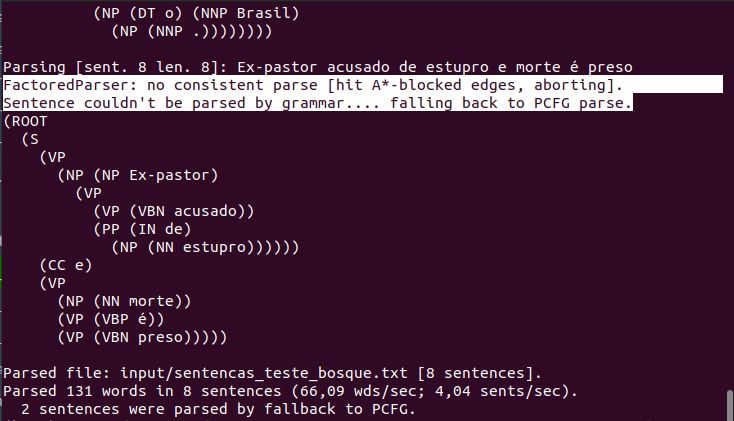
\includegraphics[width=.8\textwidth,scale=1.5]{imagens/erro_factored_parser.png}
    \caption[Erro no \textit{FactoredParser}]{Erro no \textit{FactoredParser}}
    \label{fig:bosque_erro_factored}
\end{figure}
\end{center}

\begin{center}
    \begin{figure}[!ht]
    \centering
    
    \begin{minipage}{.8\textwidth}
        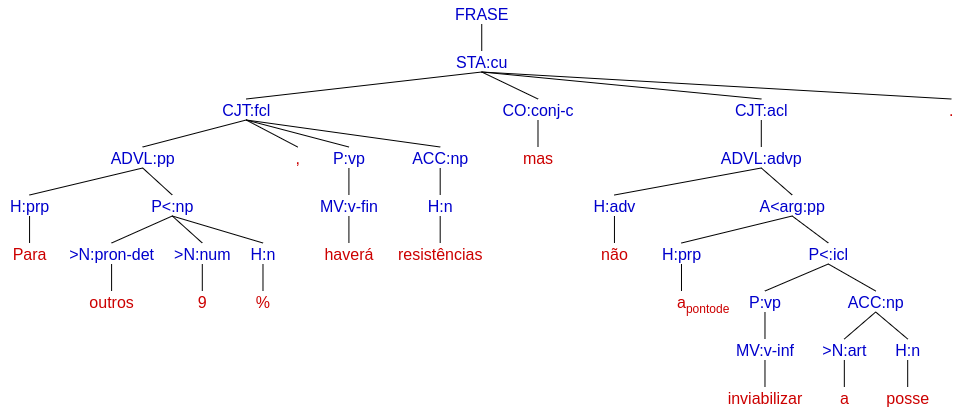
\includegraphics[width=\linewidth]{imagens/ec_bosque_perc_orig.png}
        \caption{árvore original}
    \end{minipage}
    % 
    \begin{minipage}{.8\textwidth}
        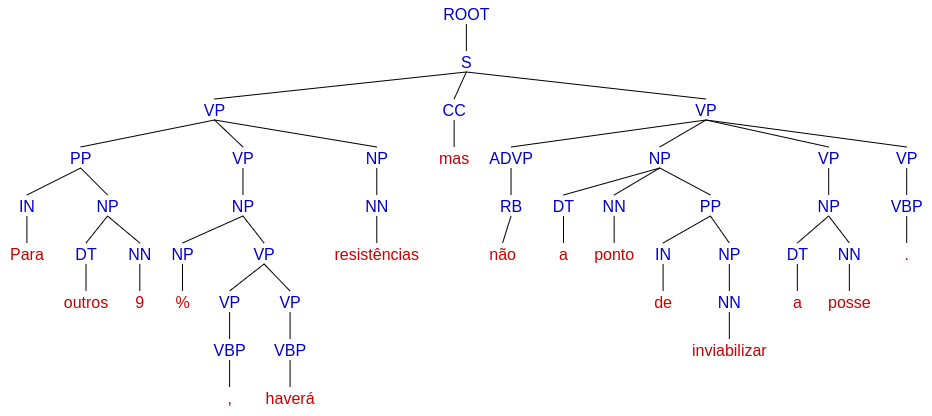
\includegraphics[width=\linewidth]{imagens/ec_bosque_perc_sp.png}
        \caption{árvore gerada pelo SP}
    \end{minipage}
    
    
    \caption[Estudo de caso BOSQUE - Sentença transduzida com sinal de porcentagem]{Estudo da sentença CF144-5, \textquote{ Para outros 9\%, haverá resistências mas não a ponto de inviabilizar a posse.}, que possui o símbolo de porcentagem. Note que, dessa vez, não há uma árvore do transdutor.}
    \label{fig:ec_bosque_perc_tree}
\end{figure}


\end{center}


\end{apendicesenv}
% ----------------------------------------------------------
% Referências bibliográficas
% ----------------------------------------------------------
\bibliography{referencias}

% ----------------------------------------------------------
% Glossário
% ----------------------------------------------------------
%
% Consulte o manual da classe abntex2 para orientações sobre o glossário.
%
%\glossary


\end{document}
